% --------------------------------------------------------
% DEFINIÇÕES DO DOCUMENTO
% --------------------------------------------------------

\documentclass[
	% -- opções da classe memoir --
	12pt,				% tamanho da fonte
	openright,			% capítulos começam em pág ímpar (insere página vazia caso preciso)
	oneside,			% para impressão em verso e anverso. Oposto a twoside
	a4paper,			% tamanho do papel.
	% -- opções da classe abntex2 --
	%chapter=TITLE,		% títulos de capítulos convertidos em letras maiúsculas
	%section=TITLE,		% títulos de seções convertidos em letras maiúsculas
	%subsection=TITLE,	% títulos de subseções convertidos em letras maiúsculas
	%subsubsection=TITLE,% títulos de subsubseções convertidos em letras maiúsculas
	% -- opções do pacote babel --
	english,			% idioma adicional para hifenização
	french,				% idioma adicional para hifenização
	spanish,			% idioma adicional para hifenização
	brazil,				% o último idioma é o principal do documento
	]{lib/abntex2}


% --------------------------------------------------------
% PACOTES
% --------------------------------------------------------
\usepackage{cmap}				% Mapear caracteres especiais no PDF
\usepackage{lmodern}			% Usa a fonte Latin Modern
\usepackage[T1]{fontenc}		% Selecao de codigos de fonte.
\usepackage[utf8]{inputenc}		% Codificacao do documento (conversão automática dos acentos)
\usepackage{lastpage}			% Usado pela Ficha catalográfica
\usepackage{indentfirst}		% Indenta o primeiro parágrafo de cada seção.
\usepackage{color}				% Controle das cores
\usepackage{graphicx}			% Inclusão de gráficos
\usepackage{lipsum}				% para geração de dummy text

\let\printglossary\relax
\let\theglossary\relax
\let\endtheglossary\relax
\usepackage{lib/update-abntex}

\usepackage[brazilian,hyperpageref]{}	 % Paginas com as citações na bibl
\usepackage{microtype} 

\usepackage{silence}
%Disable all warnings issued by latex starting with "You have..."
\WarningFilter{latex}{You have requested package}
\usepackage[alf, abnt-etal-list=0 ]{lib/abntex2cite}	% Citações padrão ABNT
\usepackage[br]{lib/nicealgo}       % Pacote para criação de algoritmos
\usepackage{lib/customizacoes}      % Pacote de customizações do abntex2

\usepackage{listings}
\usepackage[normalem]{ulem} % Strikethrough package

\usepackage{subcaption}     %para imagens com sub imagens
\usepackage{placeins}       %impedir imagem de ir para outra seção
\usepackage{url}            % Para lidar com URLs em notas de rodapé

% --------------------------------------------------------
% CONFIGURAÇÕES DE PACOTES
% --------------------------------------------------------

% Configurações do pacote listing
\renewcommand{\lstlistingname}{Código} %Mudança no caption do listing para Código
\renewcommand{\lstlistlistingname}{Lista de códigos} %Mudança no caption da lista de listings.

% Contagem de códigos sem incluir o número do capítulo
\usepackage{chngcntr}
\AtBeginDocument{\counterwithout{lstlisting}{chapter}}

% Configurações do pacote backref
\renewcommand{\familydefault}{\sfdefault}
% Usado sem a opção hyperpageref de backref
% \renewcommand{\backrefpagesname}{Citado na(s) página(s):~}
% Texto padrão antes do número das páginas
% \renewcommand{\backref}{}
% Define os textos da citação
% \renewcommand*{\backrefalt}[4]{
% 	\ifcase #1 %
% 		Nenhuma citação no texto.%
% 	\or
% 		Citado na página #2.%
% 	\else
% 		Citado #1 vezes nas páginas #2.%
% 	\fi}%


% --------------------------------------------------------
% INFORMAÇÕES DE DADOS PARA CAPA E FOLHA DE ROSTO
% --------------------------------------------------------

\titulo{DESENVOLVIMENTO DE UM JOGO 2D QUE ABORDA TEMAS DE SAÚDE MENTAL UTILIZANDO TÉCNICAS DE IA PARA O PROCESSO DE ANIMAÇÃO}
\autor{Luana Rodrigues da Silva e Lima}
\local{Bauru}
\data{Outubro/2025}
\orientador{Profa. Dra. Juliana da Costa Feitosa}
\coorientador{Prof. Dr. Seu Coorientador}
\instituicao{%
  Universidade Estadual Paulista ``Júlio de Mesquita Filho''
  \par
  Faculdade de Ciências
  \par
  Bacharelado em Ciência da Computação}
\tipotrabalho{Trabalho de Conclusão de Curso}
\preambulo{Trabalho de Conclusão de Curso do Curso de Bacharelado em Ciência da Computação da Universidade Estadual Paulista ``Júlio de Mesquita Filho'', Faculdade de Ciências, Campus Bauru.}


% --------------------------------------------------------
% CONFIGURAÇÕES PARA O PDF FINAL
% --------------------------------------------------------

% alterando o aspecto da cor azul
\definecolor{blue}{RGB}{41,5,195}

% informações do PDF
\makeatletter
\hypersetup{
     	%pagebackref=true,
		pdftitle={\@title},
		pdfauthor={\@author},
    	pdfsubject={\imprimirpreambulo},
	    pdfcreator={LaTeX with abnTeX2},
		pdfkeywords={abnt}{latex}{abntex}{abntex2}{trabalho acadêmico},
		colorlinks=true,       		% false: boxed links; true: colored links
    	linkcolor=blue,          	% color of internal links
    	citecolor=blue,        		% color of links to bibliography
    	filecolor=magenta,      		% color of file links
		urlcolor=blue,
		bookmarksdepth=4
}
\makeatother


% ---
% Posiciona figuras e tabelas no topo da página quando adicionadas sozinhas
% em um página em branco. Ver https://github.com/abntex/abntex2/issues/170
\makeatletter
\setlength{\@fptop}{5pt} % Set distance from top of page to first float
\makeatother
% ---

% ---
% Possibilita criação de Quadros e Lista de quadros.
% Ver https://github.com/abntex/abntex2/issues/176
%
\newcommand{\quadroname}{Quadro}
\newcommand{\listofquadrosname}{Lista de quadros}

\newfloat[chapter]{quadro}{loq}{\quadroname}
\newlistof{listofquadros}{loq}{\listofquadrosname}
\newlistentry{quadro}{loq}{0}

% configurações para atender às regras da ABNT
\setfloatadjustment{quadro}{\centering}
\counterwithout{quadro}{chapter}
\renewcommand{\cftquadroname}{\quadroname\space} 
\renewcommand*{\cftquadroaftersnum}{\hfill--\hfill}

\setfloatlocations{quadro}{hbtp}
% ---


% --------------------------------------------------------
% ESPAÇAMENTOS ENTRE LINHAS E PARÁGRAFOS
% --------------------------------------------------------

% O tamanho do parágrafo é dado por:
\setlength{\parindent}{1.3cm}

% Controle do espaçamento entre um parágrafo e outro:
\setlength{\parskip}{0.2cm}


% --------------------------------------------------------
% COMPILANDO O ÍNDICE
% ---------------------------------------------------
\makeindex
% ---
 
% ---
% GLOSSARIO
% ---
\makeglossaries
% ---
% Exemplo de configurações do glossairo
\renewcommand*{\glsseeformat}[3][\seename]{\textit{#1}  
 \glsseelist{#2}}
% ---
 
% --------------------------------------------------------
% INÍCIO DO DOCUMENTO
% --------------------------------------------------------

\begin{document}

% Seleciona o idioma do documento (conforme pacotes do babel)
\selectlanguage{brazil}

% Retira espaço extra obsoleto entre as frases.
\frenchspacing


% --------------------------------------------------------
% ELEMENTOS PRÉ-TEXTUAIS
% --------------------------------------------------------

% Capa
% --------------------------------------------------------
% ATENÇÃO: Se você estiver tentando alterar alguns dados da capa, como o texto
% "Campus Bauru" por exemplo, dê uma procurada no arquivo lib/customizacoes.sty
% próximo à linha 35.
% --------------------------------------------------------
\imprimircapa

% Folha de rosto
% (o * indica que haverá a ficha bibliográfica)
\imprimirfolhaderosto*

% Inserir a ficha bibliografica
\begin{fichacatalografica}
	\sffamily
	\vspace*{\fill}					% Posição vertical
	\begin{center}					% Minipage Centralizado
		\fbox{\begin{minipage}[c][7.5cm]{12.5cm}		% Largura
			\small
			\imprimirautor
			\hspace{0.5cm} \imprimirtitulo  / \imprimirautor. --
			\imprimirlocal, \imprimirdata-
			\hspace{0.5cm} \pageref{LastPage} p. : il. (algumas color.) ; 30 cm.\\
			\hspace{0.5cm} \imprimirorientadorRotulo~\imprimirorientador\\
			\hspace{0.5cm}
			\parbox[t]{\textwidth}{\imprimirtipotrabalho~--~\imprimirinstituicao,
				\imprimirdata.}\\
			\hspace{0.5cm}
			1. Tags
			2. Para
			3. A
			4. Ficha
			5. Catalográfica
			\end{minipage}}
	\end{center}
\end{fichacatalografica}

% Inserir folha de aprovação
\begin{folhadeaprovacao}
	\begin{center}
		{\ABNTEXchapterfont\large\imprimirautor}
		\vspace*{\fill}\vspace*{\fill}
		\begin{center}
			\ABNTEXchapterfont\bfseries\Large\imprimirtitulo
		\end{center}
		\vspace*{\fill}
		\hspace{.45\textwidth}
		\begin{minipage}{.5\textwidth}
			\imprimirpreambulo
		\end{minipage}%
		\vspace*{\fill}
	\end{center}
	\center Banca Examinadora
	\assinatura{\textbf{\imprimirorientador} \\ Orientador\\
		Departamento de Computação \\
		Faculdade de Ciências \\
	Universidade Estadual Paulista "Júlio de Mesquita Filho"}
	\assinatura{\textbf{Professor Convidado 1} \\
		Departamento de Computação \\
		Faculdade de Ciências \\
	Universidade Estadual Paulista "Júlio de Mesquita Filho"}
	\assinatura{\textbf{Professor Convidado 2} \\
		Departamento de Computação \\
		Faculdade de Ciências \\
	Universidade Estadual Paulista "Júlio de Mesquita Filho"}
	\begin{center}
		\vspace*{0.5cm}
		\par
		{Bauru, \_\_\_\_\_ de \_\_\_\_\_\_\_\_\_\_\_ de \_\_\_\_.}
		\vspace*{1cm}
	\end{center}
\end{folhadeaprovacao}

% Dedicatória
\begin{dedicatoria}
	\vspace*{\fill}
	\begin{flushright}
		\textit{Espaço destinado à dedicátoria do texto.} 
	\end{flushright}
\end{dedicatoria}

% Agradecimentos
\begin{agradecimentos}
	Espaço destinado aos agradecimentos.
\end{agradecimentos}

% Epígrafe
\begin{epigrafe}
	\vspace*{\fill}
	\begin{flushright}
		\textit{Espaço destinado à epígrafe.}\\
		Não esquecer autor
	\end{flushright}
\end{epigrafe}


% --------------------------------------------------------
% RESUMOS
% --------------------------------------------------------

% resumo em português
\setlength{\absparsep}{18pt} % ajusta o espaçamento dos parágrafos do resumo
\begin{resumo}
	Espaço destinado à escrita do resumo.\\
	\textbf{Palavras-chave:} Palavras-chave de seu resumo.
\end{resumo}

% resumo em inglês
\begin{resumo}[Abstract]
	\begin{otherlanguage*}{english}
		Abstract area.\\
		\textbf{Keywords:} Abstract keywords.
	\end{otherlanguage*}
\end{resumo}


% --------------------------------------------------------
% LISTA DE ILUSTRAÇÕES
% --------------------------------------------------------

% inserir lista de ilustrações
\pdfbookmark[0]{\listfigurename}{lof}
\listoffigures*
\cleardoublepage

% --------------------------------------------------------
% LISTA DE QUADROS
% --------------------------------------------------------
\pdfbookmark[0]{\listofquadrosname}{loq}
\listofquadros*
\cleardoublepage
% ---

% --------------------------------------------------------
% LISTA DE TABELAS
% --------------------------------------------------------

% inserir lista de tabelas
\pdfbookmark[0]{\listtablename}{lot}
\listoftables*
\cleardoublepage

% --------------------------------------------------------
% LISTA DE ABREVIATURAS E SIGLAS
% ---
\begin{siglas}
	\item[IA] Inteligência Artificial
	\item[S2] Sigla 2
	
\end{siglas}
% --------------------------------------------------------

% --------------------------------------------------------
% SUMÁRIO
% --------------------------------------------------------

% inserir o sumario
\pdfbookmark[0]{\contentsname}{toc}
\tableofcontents*
\cleardoublepage


% --------------------------------------------------------
% ELEMENTOS TEXTUAIS
% --------------------------------------------------------

\pagestyle{simple}

% Arquivos .tex do texto, podendo ser escritos em um único arquivo ou divididos da forma desejada
\chapter{Introdução}
\label{c.introducao}


A saúde mental é um componente crítico do bem-estar geral e ela se manifesta de forma variável em cada pessoa, de maneira muito parecida com a saúde física \cite{deleene}. Ao longo da vida, diversos determinantes contribuem para proteger, prejudicar ou deixar mais vulnerável a saúde mental do ser humano, como fatores psicológicos e biológicos individuais, circunstâncias sociais  e ambientes desfavoráveis \cite{world_2022}. 

Esse tema ganhou importância e visibilidade recentemente com a divulgação da Agenda de Desenvolvimento Sustentável 2030 da Organização das Nações Unidas (ONU), pois pela primeira vez as metas incluíram saúde mental de maneira explícita. No Objetivo de Desenvolvimento Sustentável (ODS) 3.4 foi estabelecida a meta de "promover a saúde mental e o bem-estar". Esse tema possui grandes impactos na qualidade de vida humana, pois pesquisas mostraram que condições de saúde mental são responsáveis por 13\% dos anos vividos com incapacidade e perdidos por morte prematura \cite{heymann_sprague_2023}; em 2019, uma a cada oito pessoas viveram com algum transtorno mental, um número que aumentou consideravelmente por causa da pandemia do COVID-19 \cite{mentalDisorders_2022}. 

Jogos Sérios são jogos cujo propósito não é apenas entretenimento, mas também a exploração ativa de problemas sociais \cite{abt1987serious}. Eles são utilizados para diversas finalidades: auxiliar no processo educacional, ajudar pacientes a entender sua condição atual e sua reabilitação, promover a conscientização do público para problemas psicológicos e emocionais, etc. Além disso, uma categoria recente de jogos vem ganhando destaque: jogos empáticos. Esses jogos priorizam, através de mecânicas, trazer a experiência de como é estar no lugar de outra pessoa. O aspecto interativo que os jogos trazem permite que o jogador participe ativamente do conteúdo mostrado, não sendo apenas observadores passivos, mas sim participantes afetados pelos eventos do universo. Dessa forma, é possível fazer com que o usuário tenha interesse em tópicos relacionados à saúde mental (como o luto e transtornos mentais) e ter uma visão mais empática sobre esse tema \cite{10.1145/3638067.3638104}.

O desenvolvimento de jogos 2D envolve a criação de um jogo que exista num espaço bidimensional, onde todos os componentes são representados usando dois eixos. De acordo com \citeonline{article}, apesar de estarmos numa era dominada por gráficos 3D, os jogos 2D mantêm sua popularidade. Isso ocorre pois são mais baratos de serem produzidos, sendo o melhor mercado para um desenvolvedor independente \cite{book}.

A Inteligência Artificial (IA) é um campo rico e diverso, que possui aplicabilidade em várias vertentes como automóveis, saúde, entretenimento, educação, segurança, entre outras. A IA foca em aprender com experiências e alterar seu processamento e comportamento baseado em seu aprendizado. Além disso, é considerada a próxima revolução industrial na área de entretenimento e também é capaz de aumentar a eficiência automatizando numerosas tarefas repetitivas \cite{articleIAEntretenimento}. Na indústria de jogos, a IA é utilizada para  gerar comportamentos responsivos, adaptativos e inteligentes para personagens não jogáveis (em inglês, NPCs) \cite{IA_jogos}. De acordo com \citeonline{jorapur2024evolution}, ela também é implementada para adaptar a história dependendo do comportamento do jogador, para criação de diferentes conteúdos do jogo como níveis e mundos infinitos e para ajustar a dificuldade de acordo com a performance do player. Além disso, é usada para fazer animações de personagem \cite{xian2023automated}.

Nesse contexto, o projeto visa desenvolver um jogo sério 2D que utiliza IA para fazer as animações dos personagens, e que aborda temas de saúde mental para trazer uma visão mais empática e conscientizar sobre esse assunto. 







 
 
  
\chapter{Revisão bibliográfica}
\label{c.revisao}

\section{Saúde mental e mídia digital}
\label{s.saudeMental}


\section{Desenvolvimento de jogos 2D}
\label{s.jogos2D}


\section{Inteligência Artificial Aplicada à Animação}
\label{s.IAanimação}


% LLM
% flow matching
%GPT

\chapter{Metodologia}
\label{c.metodologia}

%   ---------------------   EDITAR PARA O QUE REALMENTE ACONTECEU -------------------

Inicialmente, será elaborado o documento GDD e o projeto de arquitetura de software, que contribuem para a organização da estrutura, roteiro, cenários e personagens do jogo. Isso será feito de forma paralela com um levantamento bibliográfico mais aprofundado sobre saúde mental, traumas, problemas emocionais, distúrbios mentais e mecanismos de enfrentamento saudáveis.

Depois que os documentos forem elaborados, será iniciado o desenvolvimento do jogo, desenhando o ambiente de cada cena e programando cada mecânica. Quando o levantamento bibliográfico sobre saúde mental for concluído, uma pesquisa sobre modelos de IA para animação será feita, analisando quais as técnicas utilizadas por cada um, as vantagens, as desvantagens e o foco. Após a pesquisa, será escolhido um modelo para ser treinado, implementado e modificado conforme necessário. O treinamento será feito de forma paralela com o desenvolvimento do jogo. Após a IA ter sido treinada, ela será utilizada para fazer as animações dos personagens do jogo. Durante o estudo, treinamento e implementação do modelo da IA, será feita uma análise de como o modelo ajuda no cenário de animações 2D, documentando qualquer modificação feita. Ao longo do desenvolvimento, serão realizados diversos testes para verificar se o comportamento está de acordo com o esperado. 

A partir do momento em que o jogo for concluído, serão realizados testes finais para verificar o funcionamento correto de todos os elementos, fazendo ajustes se necessário. O planejamento da ordem em que cada atividade será realizada é demonstrado pela Figura \ref{f.Diagrama}.

\begin{figure}[htbp]
	\caption{\small Fluxograma das etapas}
	\centering
	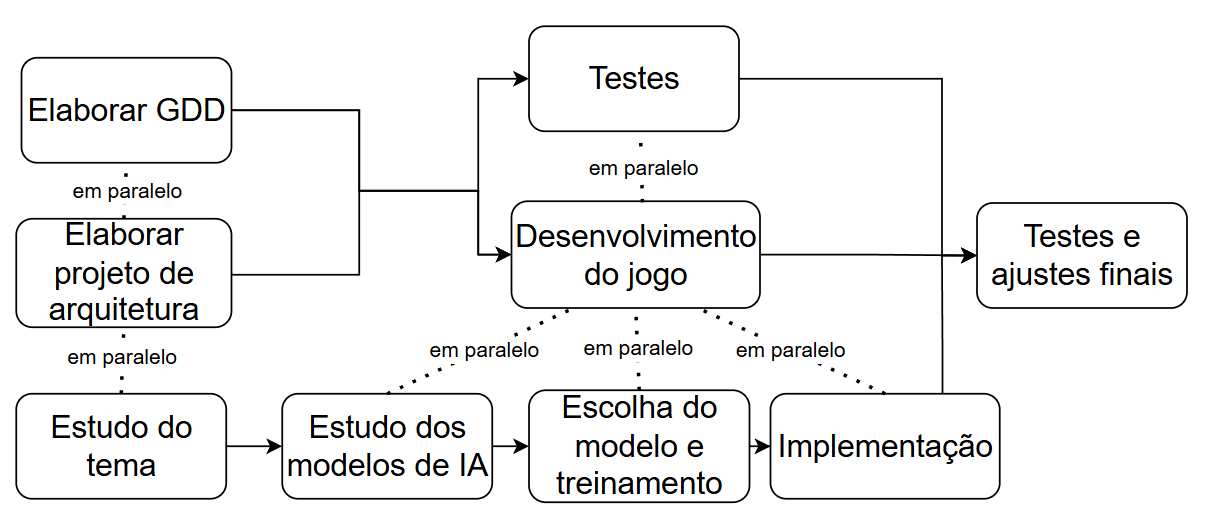
\includegraphics[width=1\linewidth]{figs/Diagrama.PNG}
	\label{f.Diagrama}
	\legend{\small Fonte: Elaborada pela autora.}
\end{figure}

%   ------------------------------------------------------------------------
\FloatBarrier
\section{Metodologia de desenvolvimento do jogo}
\label{s.jogo}

\FloatBarrier
\section{Metodologia de Análise das Ferramentas de IA}
\label{s.ia}


Para conduzir a análise comparativa das ferramentas de IA, a metodologia foi estruturada em etapas, partindo de uma seleção ampla de ferramentas até uma avaliação aprofundada das mais promissoras.

Inicialmente, foram estabelecidos os seguintes critérios de seleção para a escolha de ferramentas:

\begin{itemize}
\item Capacidade de criar vídeos ou imagens que pudessem ser usados para a animação 2D;
\item Disponibilidade de um modelo de acesso gratuito, ainda que com limitações de uso;
\item Possibilidade de usar uma imagem pré-existente (do personagem ou objeto) como referência, para consistência visual; e
\item Acessível para um usuário sem conhecimento aprofundado na ferramenta.
\end{itemize}

%------------------------ CHECAR SE NÃO OLHOU NENHUMA NOVA NÃO MENCIONADA ----------------
Com base nesses critérios, foram selecionados os seguintes softwares como candidatos para a produção de animação 2D: CGDream \cite{cgdream_2025}, ChatGPT \cite{chatgpt_2025}, OpenArtAI\cite{openArtai_2025}, geminiPro \cite{gemini_2025}, God Mode AI \cite{godmodeanimation2024}, PixelLab \cite{pixelLab}, PixieHaus \cite{pixie.haus_2025}, Rosebud AI \cite{rosebud}, Animated Drawings \cite{animatedDrawings}, Vidu \cite{viduai_2024}, AI Sprite Sheet Maker \cite{segmind} e SpriteSheetGPT \cite{spritesheetgpt-free}. 


O processo de análise foi dividido em duas fases. A primeira fase consistiu em uma análise geral de cada ferramenta, verificando os recursos grátis disponíveis, as opções de customização existentes e a capacidade de gerar uma animação 2D útil para o jogo em desenvolvimento a partir de um sprite de referência. Essa triagem inicial permitiu descartar algumas ferramentas que provaram não ser capazes de alcançar o resultado desejado, sobrando apenas as candidatas mais promissoras. Um desafio descoberto nesta etapa foi a limitação de uso do modelo gratuito de muitas plataformas, o que restringiu o número de testes comparativos e reduziu o número de gerações.

Na segunda fase, foi realizado um aprofundamento das ferramentas restantes. Foram conduzidos testes iterativos com diversos prompts (a maioria em inglês para melhores resultados) e imagens de referências nas plataformas que não possuíam um limite para o uso gratuito, ou este era muito alto. Para as plataformas mais restritas, os resultados que chegavam mais perto do desejado eram usados como referência para os outros softwares. As animações satisfatórias foram implementadas no jogo, com o uso de ferramentas auxiliares para converter ou ajustar o formato do arquivo e para pequenas edições na imagem.

%------------- CHECAR SE NÃO CRIOU NENHUMA ANIMAÇÃO NOVA NÃO MENCIONADA ----------------
Foram criadas animações com IA para alguns elementos do jogo: o personagem Pablo (Figura \ref{fig:Pablo}), que realiza as ações de andar, pular, virar de costas e sentar; a personagem Luz; e a porta (Figuras \ref{fig:portaA}, \ref{fig:portaB}) e \ref{fig:portaC}, que executa os movimentos de abrir e fechar. Os resultados adequados foram implementados no jogo.


\begin{figure}[htbp]
    \centering
    \caption{\small Sprite do Pablo}
    
\includegraphics[width=0.3\linewidth]{figs/sprites/Pablo.PNG}
    \label{fig:Pablo}
    \legend{\small Fonte: Elaborada pela autora.}
\end{figure}


\begin{figure}[htbp]
    \centering
    \caption{\small Sprite da Luz}
    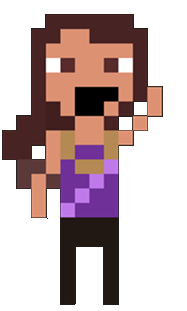
\includegraphics[width=0.3\linewidth]{figs/sprites/irma.PNG}
    \label{fig:Luz}
    \legend{\small Fonte: Elaborada pela autora.}
\end{figure}


\begin{figure}[htbp]
    \centering
    \begin{minipage}{0.45\textwidth}
    \caption{\small Sprite da porta A em front view (vista frontal, em inglês)}
    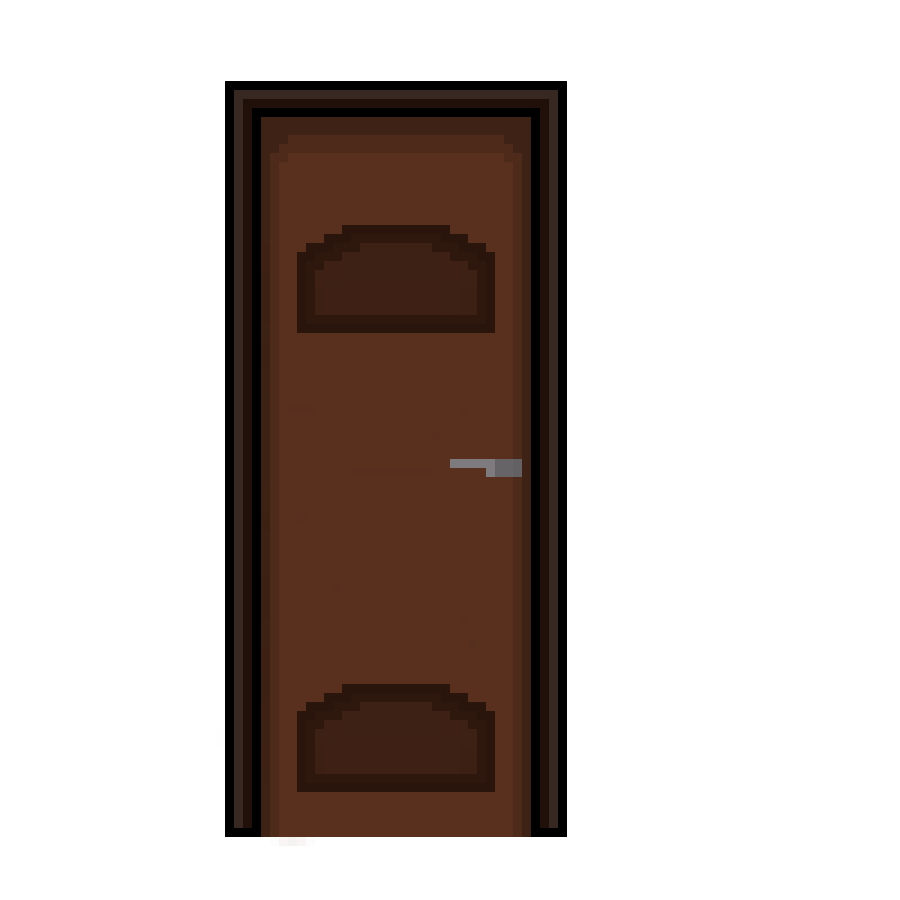
\includegraphics[width=1\linewidth]{figs/sprites/Porta front view.png}
    \label{fig:portaA}
    \legend{\small Fonte: Elaborada pela autora.}
    \end{minipage}\hfill
    \begin{minipage}{0.45\textwidth}
    \caption{\small Sprite da porta B em side view (vista lateral, em inglês)}
    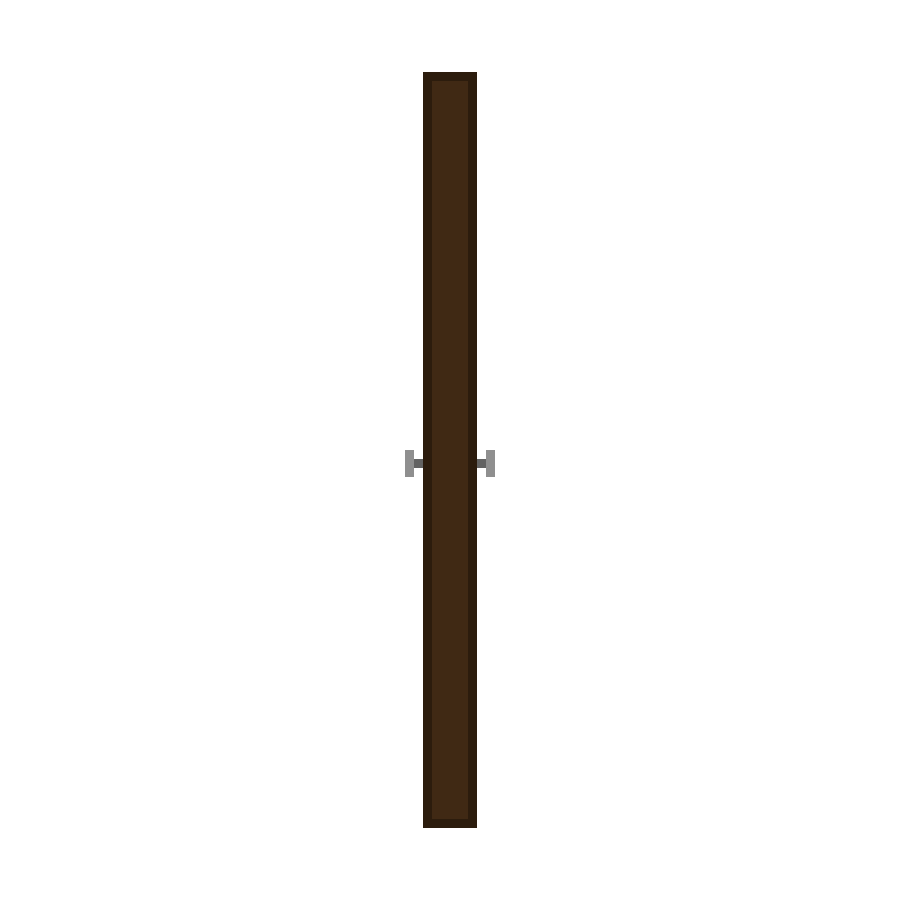
\includegraphics[width=1\linewidth]{figs/sprites/Porta side view.png}
    \label{fig:portaB}
    \legend{\small Fonte: Elaborada pela autora.}
    \end{minipage}\hfill
\end{figure}


\begin{figure}[htbp]
    \centering
    \caption{\small Sprites da porta C}
    \label{fig:portaC}
    \begin{subfigure}{0.45\textwidth}
    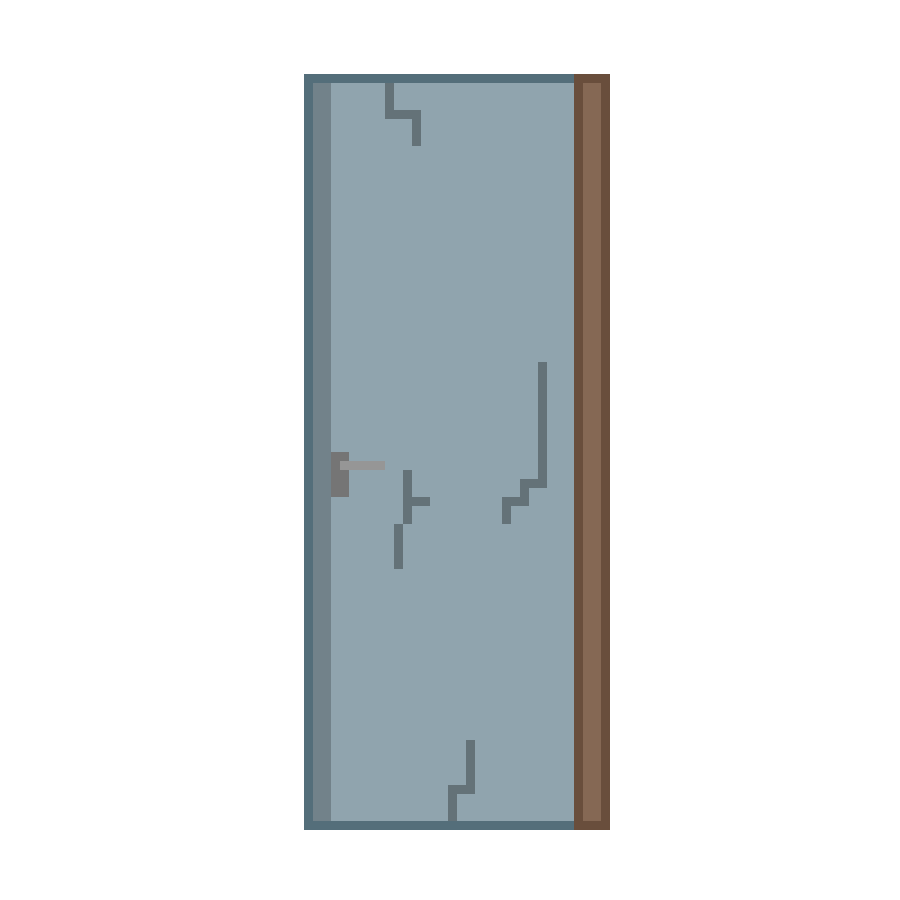
\includegraphics[width=1\linewidth]{figs/sprites/referencia_porta_tutorial (1).png}
    \caption{\small Sprite da porta C aberta em side view}
    \label{fig:portaCAberto}
    \end{subfigure}\hfill
    \begin{subfigure}{0.45\textwidth}
    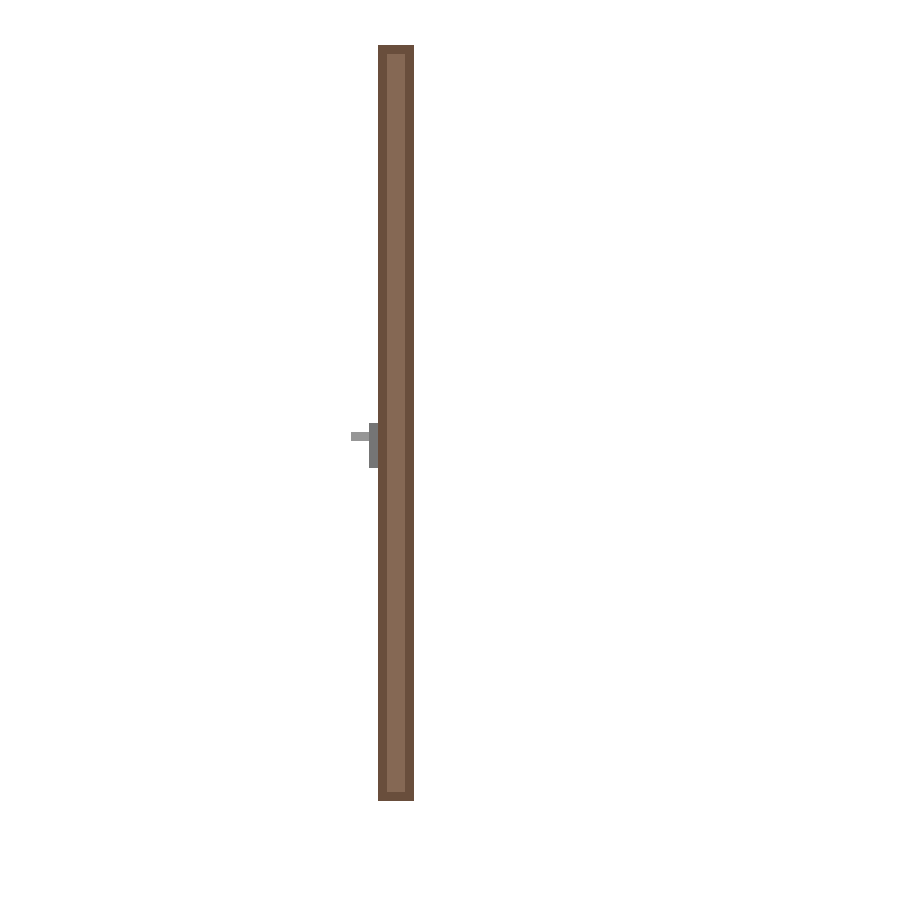
\includegraphics[width=1\linewidth]{figs/sprites/referencia_porta_tutorial (2).png}
    \caption{\small Sprite da porta C fechada em side view}
    \label{fig:portaCFechado}

    \end{subfigure}\hfill
    \legend{\small Fonte: Elaborada pela autora.}
\end{figure}

Ao final do processo, as ferramentas mais satisfatórias serão comparadas e avaliadas pelos seguintes critérios:

\begin{itemize}
\item Foco em 2D;
\item Consistência com o estilo e cores da imagem de referência;
\item Facilidade de uso e curva de aprendizagem;
\item Precisão de movimento e fidelidade ao prompt;
\item Qualidade estética;
\item Nível de customização;
\item Eficiência;
\item Capacidade de produzir resultado pixel perfect (todos os pixels tem o mesmo tamanho); e
\item Capacidade de edição e refinamento do material gerado.
\end{itemize}

\chapter{Análise comparativa de ferramentas de IA para animação 2D}
\label{c.ferramentas}




%   ------------------------------------------------------------------------
\FloatBarrier
\section{Visão geral da análise comparativa}
\label{s.visaoAnalise}

Como já foi mencionado, a aplicação de IA para a criação de animações 2D não foi muito explorada, tendo um potencial muito grande a ser descoberto. Atualmente, a maioria das ferramentas generativas de vídeo é voltada para ambientes tridimensionais e realistas. Diante desse cenário, esta análise busca investigar a capacidade e o resultado das tecnologias atuais quando aplicadas ao contexto da animação 2D para um jogo.

Durante a análise preliminar, uma das ferramentas foi imediatamente descartada do estudo por não ser capaz de gerar resultados. A ferramenta AI Sprite Sheet Maker, encontrada na plataforma segmind, foi inicialmente selecionada por seu foco na criação do sprite sheet de um personagem a partir de uma única imagem. A funcionalidade apresentada na página da ferramenta (Figura \ref{fig:segmindDemo} do Apêndice \ref{ap.telasIA}) indicava a geração do personagem anexado em diferentes posições, não formando nenhuma ação específica. Esse é um recurso com potencial para a criação de imagens de referência, embora não tenha capacidade de geração direta de animações. A plataforma segmind disponibiliza \$1 de crédito gratuito, enquanto o custo por geração com este modelo é de aproximadamente \$0.01 (Figura \ref{fig:segmindLimitado} do Apêndice \ref{ap.telasIA}). Em teoria, o saldo inicial seria o suficiente para múltiplos testes, porém, ao tentar gerar o sprite sheet, o sistema retornou uma mensagem de erro informando que os créditos eram insuficientes. Diante da impossibilidade de continuar a análise e teste da ferramenta, a mesma foi descartada do estudo. As capturas de tela da interação completa podem ser consultadas na Figura \ref{fig:segmind1} do Apêndice \ref{ap.telasIA}.  


Nas seções seguintes, é apresentada uma análise detalhada das demais ferramentas, sendo o objetivo desse capítulo responder a uma série de questões-chave:

\begin{itemize}
    \item Avaliar se ferramentas com foco em realismo podem ser adaptadas para a animação 2D; 
    \item Analisar o nível de desenvolvimento das ferramentas que possuem foco em 2D; 
    \item Determinar o grau de consistência que as IAs mantêm em relação a um design de personagem pré-existente e a um estilo artístico específico; 
    \item Verificar a possibilidade de utilizar ferramentas de geração de imagem para auxiliar na animação, incluindo a criação sequencial de quadros e a geração de novas poses ou vistas do personagem (como a vista lateral a partir da frontal); e
    \item Investigar a capacidade das ferramentas de gerar uma imagem pixel perfect, característico do estilo pixel art.
\end{itemize}

Ao final, busca-se mostrar o papel prático dessas tecnologias no processo de desenvolvimento de um jogo, posicionando-as não como uma possível substituição ao trabalho artístico, mas como ferramentas potenciais para otimizar e facilitar o complexo processo de animação.


%   ------------------------------------------------------------------------
\FloatBarrier
\section{Análise do RosebudAI}

A ferramenta RosebudAI foi selecionada por demonstrar ter foco na criação de sprite sheets, especificamente para jogos. Na sua página inicial (Figura \ref{fig:rosebudInicial} no Apêndice \ref{ap.telasIA}), afirmações como "Use IA para criar sprites para seu jogo" apontavam para a capacidade da plataforma em criar animações para um personagem. No entanto, a análise revelou uma ferramenta com múltiplas funcionalidades que, em todos os testes, falhou em produzir um sprite sheet 2D consistente a partir de uma imagem de referência. 

Os testes foram realizados em junho, focando no ambiente principal da plataforma. O objetivo principal era produzir o sprite sheet ou animação do walking cycle (ciclo de caminhada, em inglês) do personagem utilizando o sprite de Pablo em front view (apresentado anteriormente na Figura \ref{fig:Pablo}). Na primeira tentativa, em vez de um sprite sheet, a ferramenta apresentou um protótipo de jogo 3D, incluindo um script de 600 linhas de código (interação completa pode ser consultada na Figura \ref{fig:rosebud1} do Apêndice \ref{ap.telasIA}). O personagem gerado (Figura \ref{fig:rosebudJogo} manteve vagamente as cores da referência, porém com um estilo cúbico inadequado, em uma aparente tentativa de emular o estilo pixel art em um ambiente tridimensional.

\begin{figure}[htbp]
    \centering
    \caption{\small Resultado do teste inicial}
    \label{fig:rosebudJogo}
    \begin{subfigure}{0.3\linewidth}
        \centering
        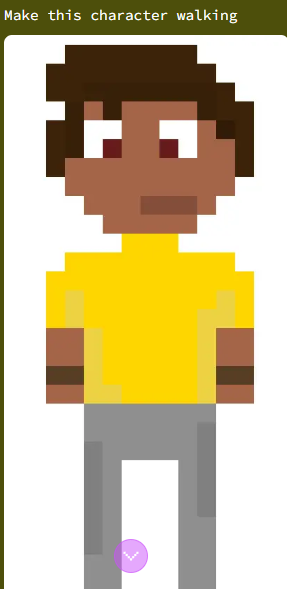
\includegraphics[width=1\linewidth]{figs/rosebud/principal1.PNG}
        \caption{\small Prompt e imagem de referência.}
        \label{fig:rosebudJogoPrompt}
    \end{subfigure} \hfill
        \begin{subfigure}{0.65\linewidth}
        \centering
        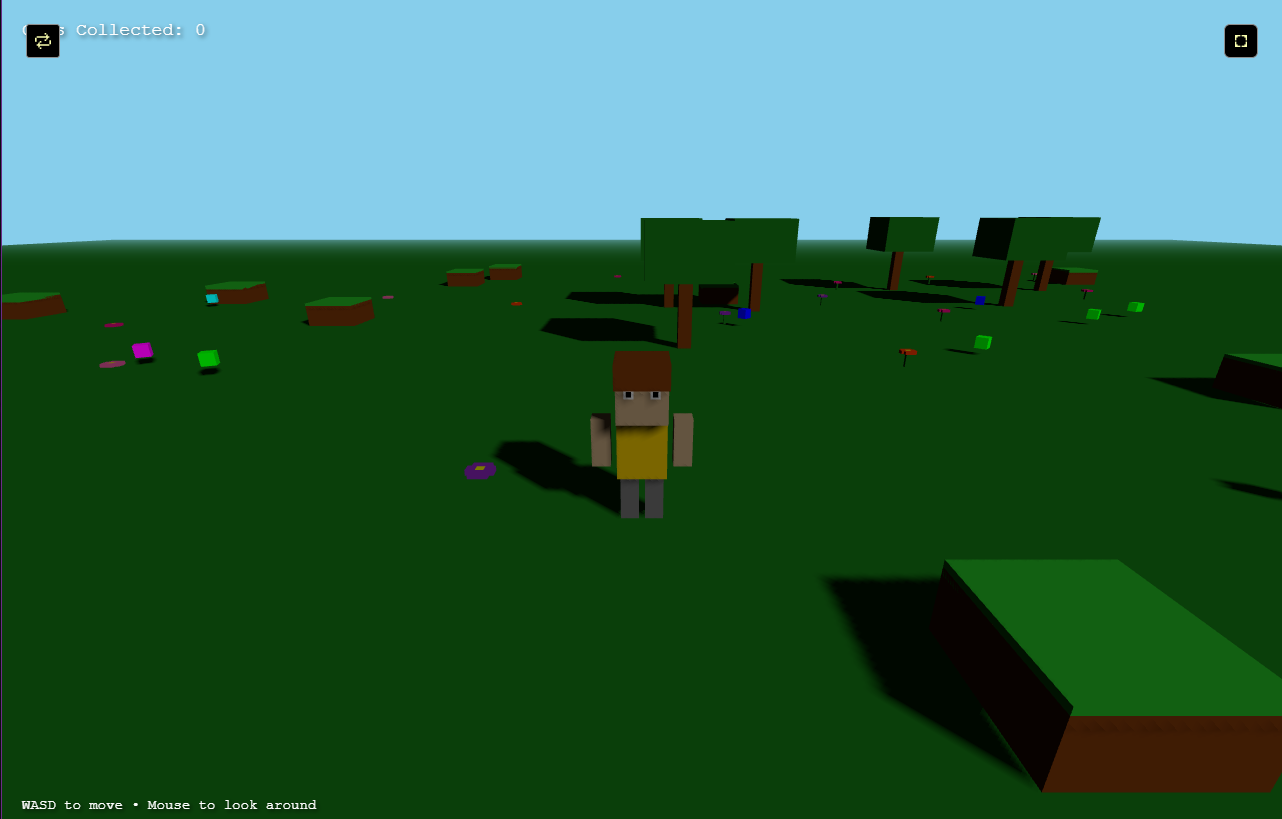
\includegraphics[width=1\linewidth]{figs/rosebud/principal2.PNG}
        \caption{\small Interface do jogo gerado.}
        \label{fig:rosebudJogoJogo}
    \end{subfigure}

    \legend{\small Fonte: Elaborada pela autora.}
\end{figure}


Em uma tentativa subsequente, com um prompt ajustado para especificar um cenário 2D e manter a consistência do personagem, a ferramenta produziu uma animação de baixa qualidade\footnote{https://drive.google.com/file/d/1yPtpKDM2CYCaxSqFJr3NFbVswduzkfTY/view?usp=sharing}, na qual metade da imagem de referência é apenas deslocada horizontalmente pela tela, alternando entre a parte inferior ou superior visível na tela, como é demonstrado na Figura \ref{fig:rosebudAnimacao}. A análise dos quadros revelou que  a IA interpretou a imagem de referência como se fosse um sprite sheet completo de dois quadros, dividindo-a ao meio e alternando entre as metades superior e inferior. As imagens completas desse teste podem ser consultadas na Figura \ref{fig:rosebud2} no Apêndice \ref{ap.telasIA}.

\begin{figure}[htbp]
    \centering
    \caption{\small Animação gerada pelo Rosebud AI}
    \label{fig:rosebudAnimacao}
    
    \begin{subfigure}{0.45\linewidth}
        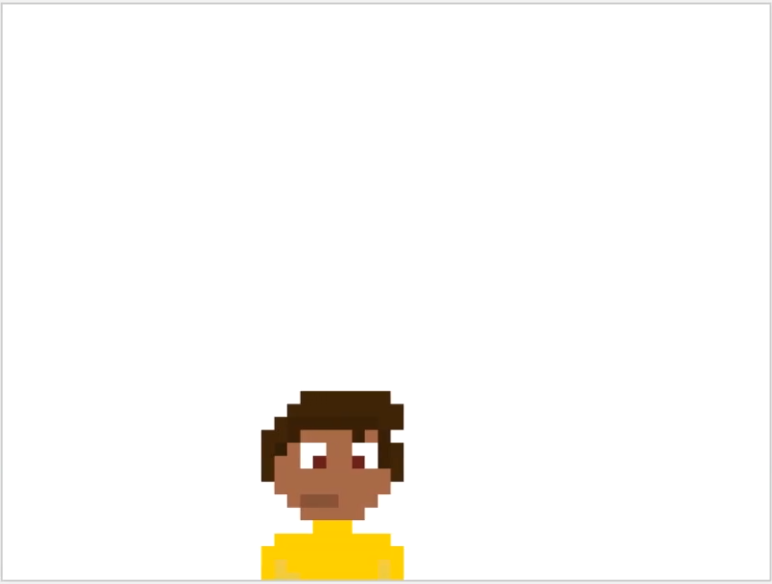
\includegraphics[width=1\linewidth]{figs/rosebud/rosebud_resultado_tela3_1.PNG}
        \caption{\small Frame 1 (metade superior).}
        \label{fig:rosebudFrame1}
    \end{subfigure}
    \begin{subfigure}{0.45\linewidth}
        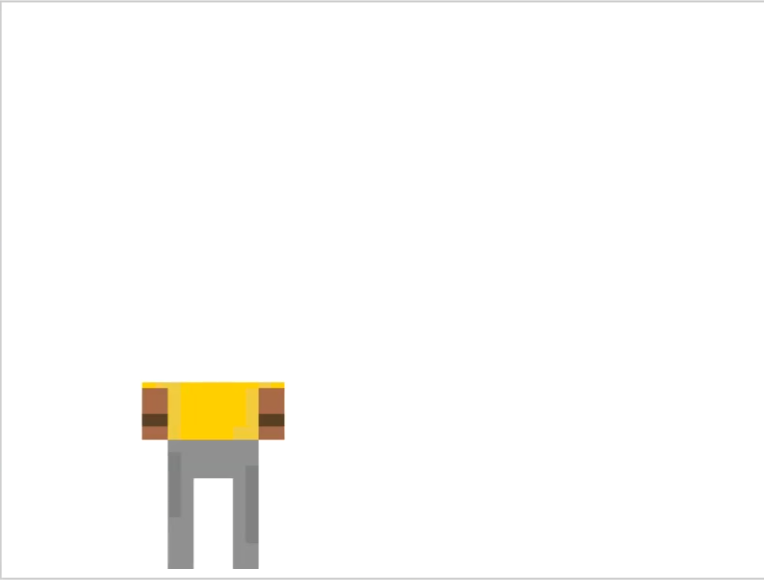
\includegraphics[width=1\linewidth]{figs/rosebud/rosebud_resultado_tela3_2.PNG}
        \caption{\small Frame 2 (metade inferior).}
        \label{fig:rosebudFrame2}
    \end{subfigure}

    \legend{\small Fonte: Elaborada pela autora, utilizando a ferramenta Rosebud AI.}
\end{figure}

Diante desse resultado, os prompts foram ajustados para especificar a criação de um sprite sheet do personagem em várias posições diferentes. Após algumas interações sem sucesso no ambiente principal, que podem ser consultadas na Figura \ref{fig:rosebud3} no Apêndice \ref{ap.telasIA}, a análise foi direcionada para uma seção separada dedicada à geração de assets (Figuras \ref{fig:rosebudPrincipal} e \ref{fig:rosebudAssets} no Apêndice \ref{ap.telasIA}). O primeiro teste nesta seção resultou na geração de um sprite único que desconsiderou completamente a imagem de referência, criando um personagem novo em um estilo distinto.

Com os testes voltados para a área de assets (interação completa mostrada pelas Figuras \ref{fig:rosebud4} no Apêndice \ref{ap.telasIA}), a ferramenta específica para geração de imagens demonstrou desconsiderar a imagem de referência, apresentando um personagem completamente novo em um estilo distinto. Além disso, foi gerado apenas um sprite em vez do sprite sheet do personagem andando. A tentativa de refinar os prompts, utilizando a IA principal para descobrir como referenciar a imagem corretamente, também levou a resultados insatisfatórios. Conforme demonstrado na Figura \ref{fig:rosebudResultadosFinais}, os sprite sheets gerados apresentaram falhas graves, como a mudança do cenário e inconsistência entre os quadros, além de ainda desconsiderar a referência. A documentação completa destes testes se encontra nas Figuras \ref{fig:rosebud4} e \ref{fig:rosebud5} do Apêndice \ref{ap.telasIA}.

\begin{figure}[htbp]
    \centering
    \caption{\small Resultados finais}
    \label{fig:rosebudResultadosFinais}
    \begin{subfigure}{0.45\textwidth}
    \caption{\small Sprite sheet com cenário mudando e frames faltando}
    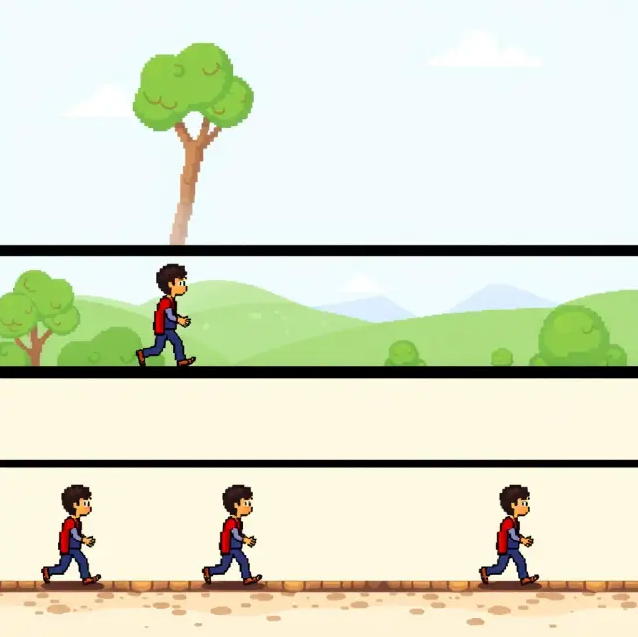
\includegraphics[width=1\linewidth]{figs/rosebud/rosebud_resultado_tela7.PNG}
    \label{fig:rosebudSpriteSheetFrameFaltando}

    \end{subfigure}\hfill
    \begin{subfigure}{0.45\textwidth}
    \caption{\small Sprite sheet com frames inconsistentes entre si}
    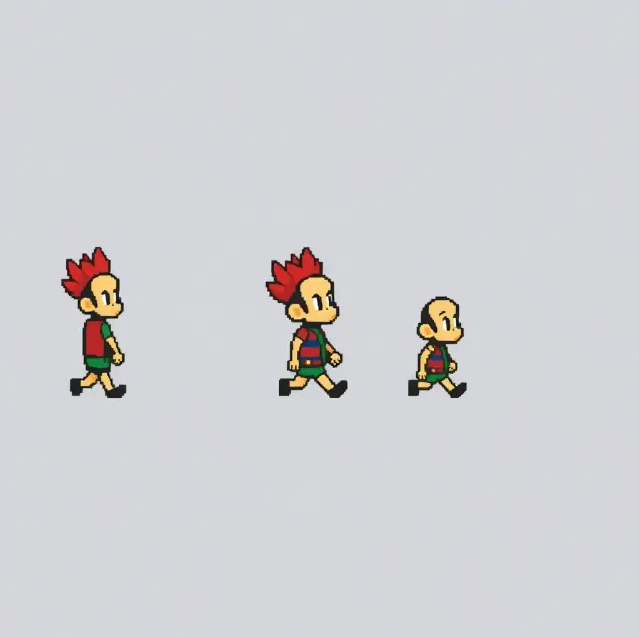
\includegraphics[width=1\linewidth]{figs/rosebud/rosebud_resultado_tela8.PNG}
    \label{fig:rosebudSpriteSheetInconsistente}
    \end{subfigure}\hfill
    \legend{\small Fonte: Elaborada pela autora, utilizando a ferramenta Rosebud AI.}
\end{figure}


Considerando que nenhuma das abordagens produziu um resultado satisfatório, a ferramenta foi descartada para esse estudo. Embora não seja viável para a criação de animações 2D personalizadas, a plataforma  demonstra potencial para a prototipagem rápida de jogos simples para usuários que não possuem conhecimento em programação.

%   ------------------------------------------------------------------------
\FloatBarrier
\section{SpriteSheetGPT}
\label{s.spritesheetGPTApendice}

\begin{figure}[htbp]
    \centering
    \caption{\small Tela do SpriteSheetGPT quando chega no limite de uso}
    \label{fig:yesAILimitado}
    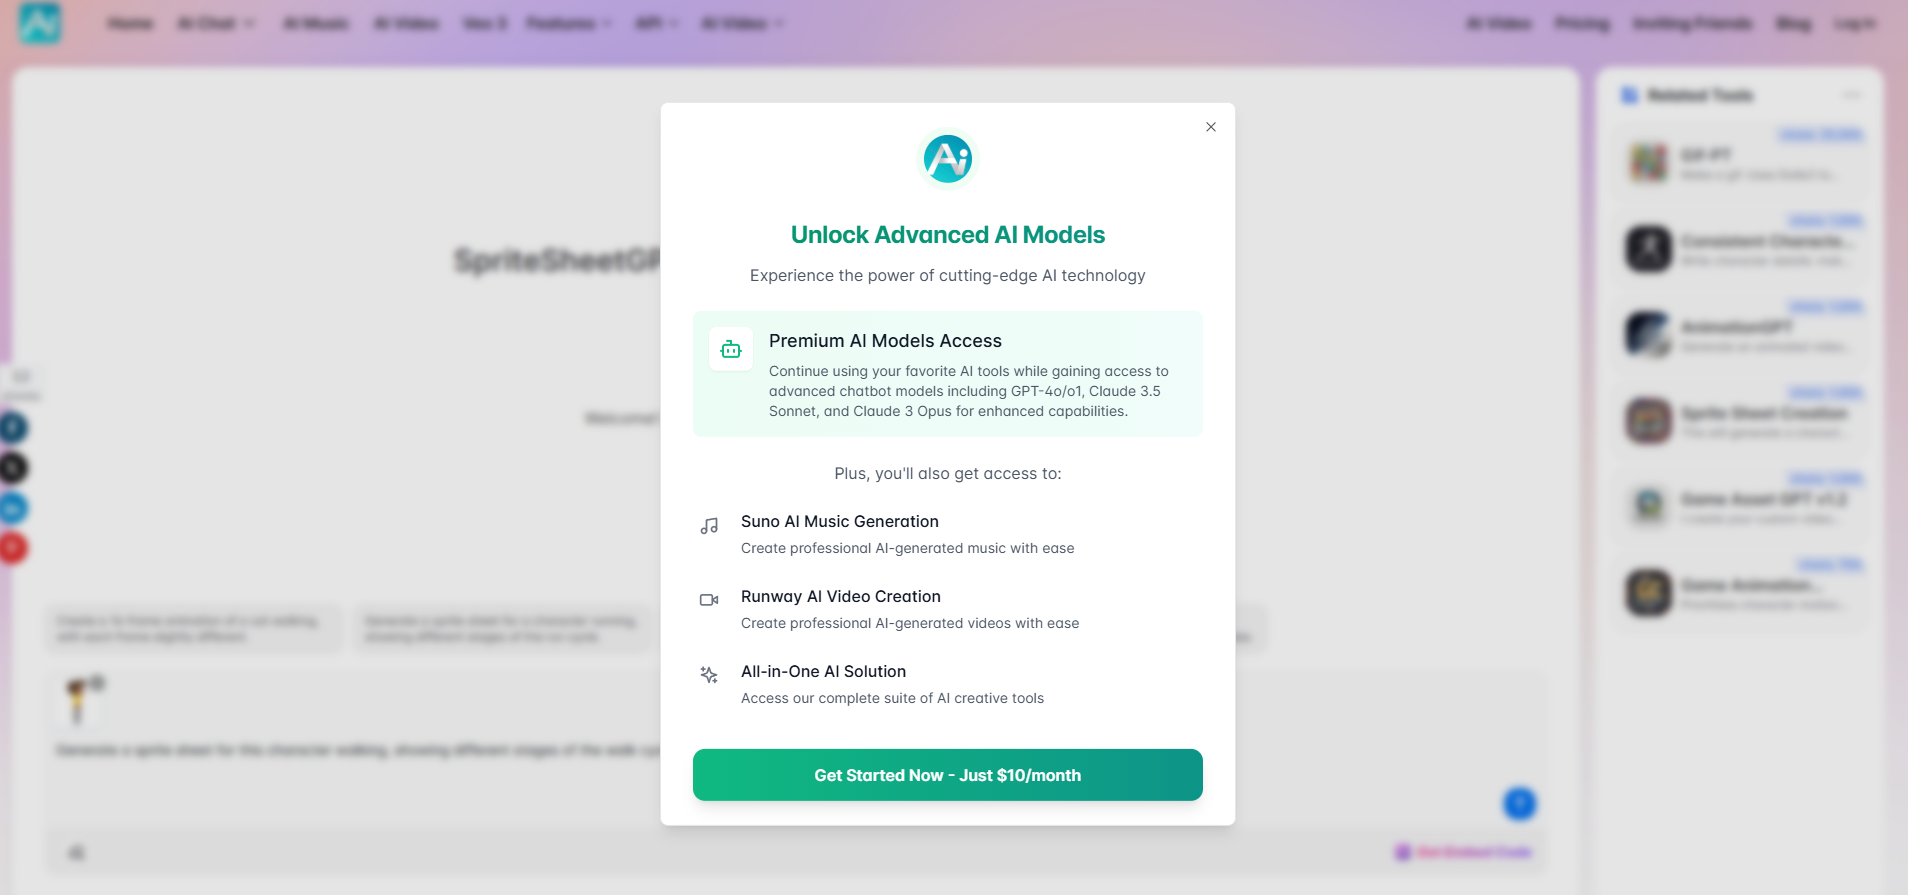
\includegraphics[width=1\linewidth]{figs/yesAI/telaLimitado.PNG}
    \legend{\small Fonte: Elaborada pela autora.}
\end{figure}

\begin{figure}[htbp]
    \centering
    \caption{\small Processo da utilização do SpriteSheetGPT em junho/2025}
    \label{fig:yesAI1}

    \begin{subfigure}{1\linewidth}
        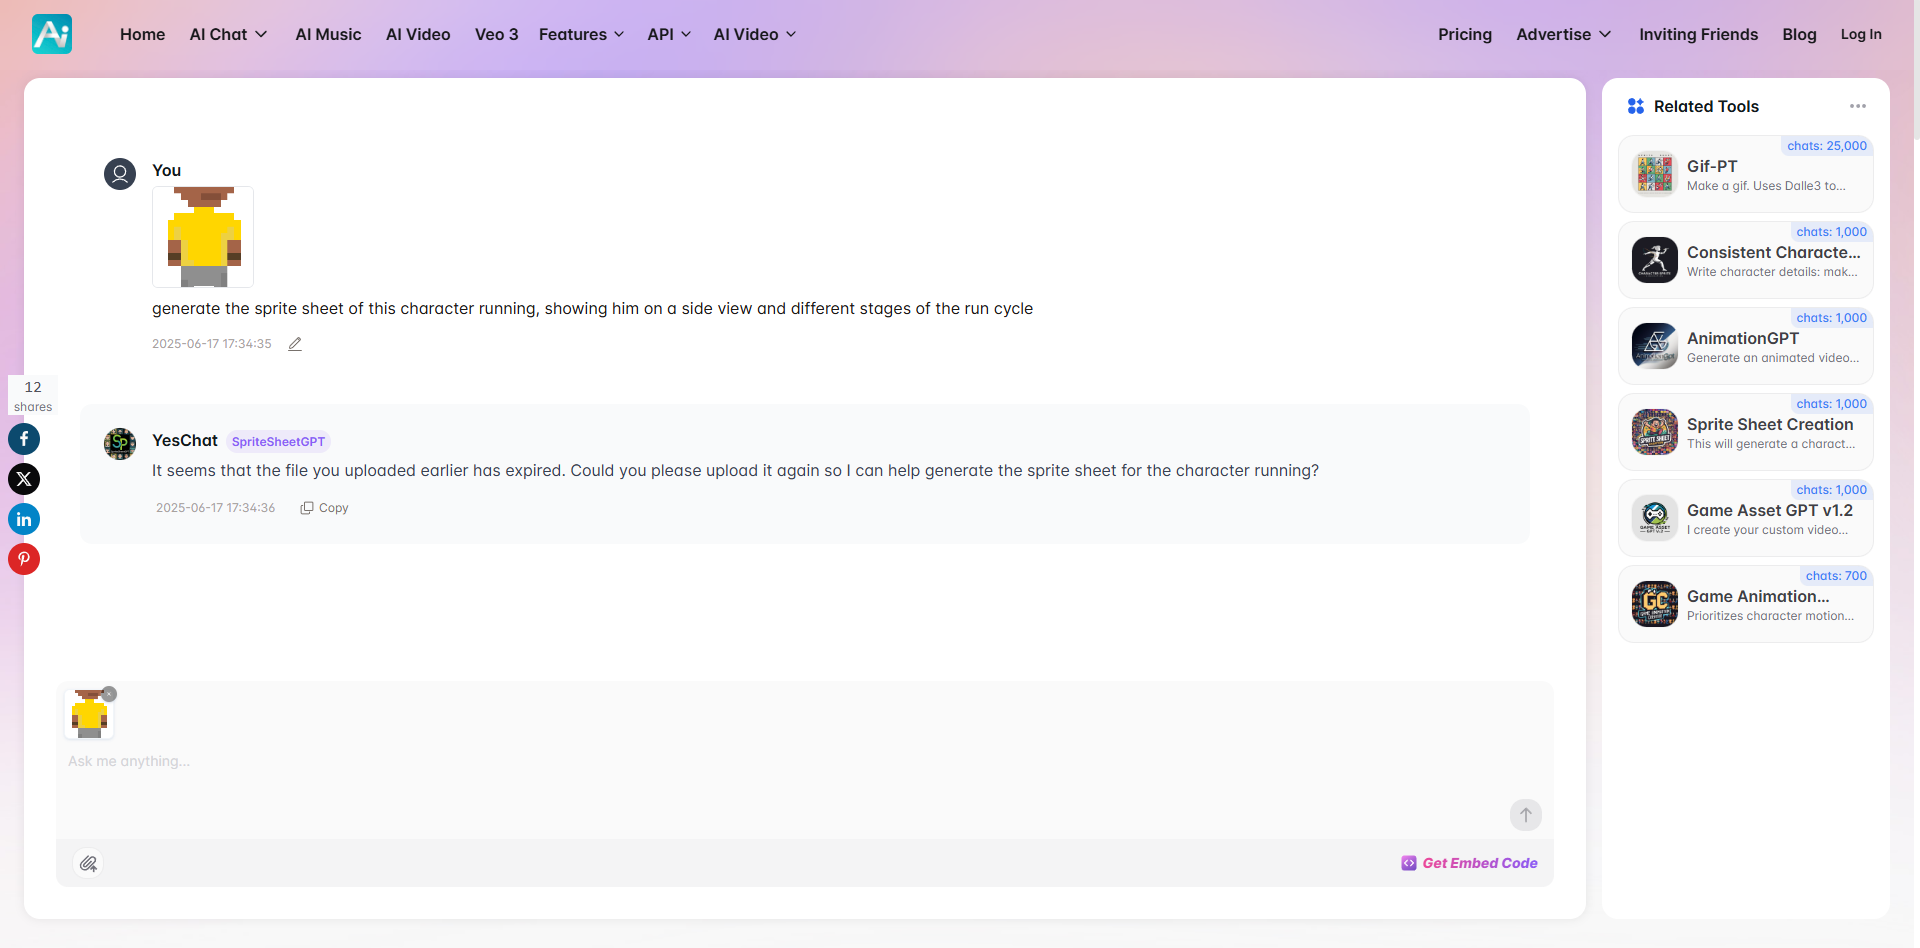
\includegraphics[width=1\linewidth]{figs/yesAI/tela1.PNG}
        \caption{\small Ferramenta solicitando o reenvio da imagem de referência.}
        \label{fig:yesAI1a}
    \end{subfigure}
    \begin{subfigure}{1\linewidth}
        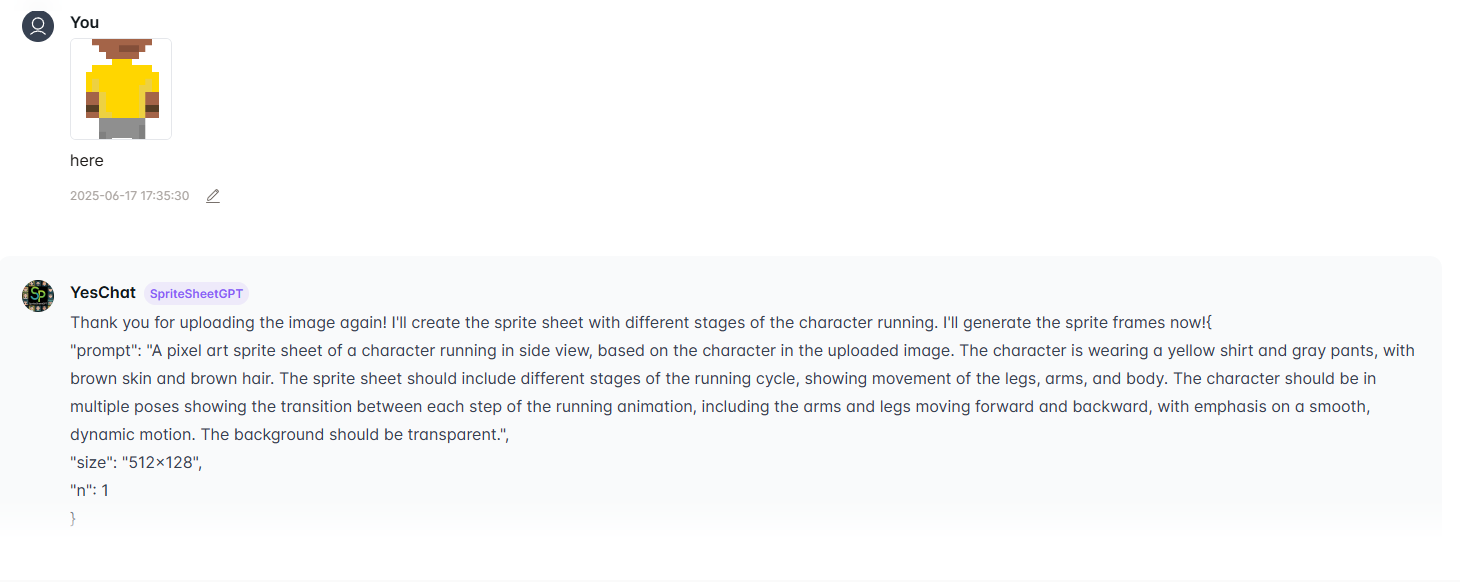
\includegraphics[width=1\linewidth]{figs/yesAI/tela2.PNG}
        \caption{\small IA descrevendo textualmente o sprite sheet em vez de gerá-lo.}
        \label{fig:yesAI1b}
    \end{subfigure}
    \begin{subfigure}{1\linewidth}
        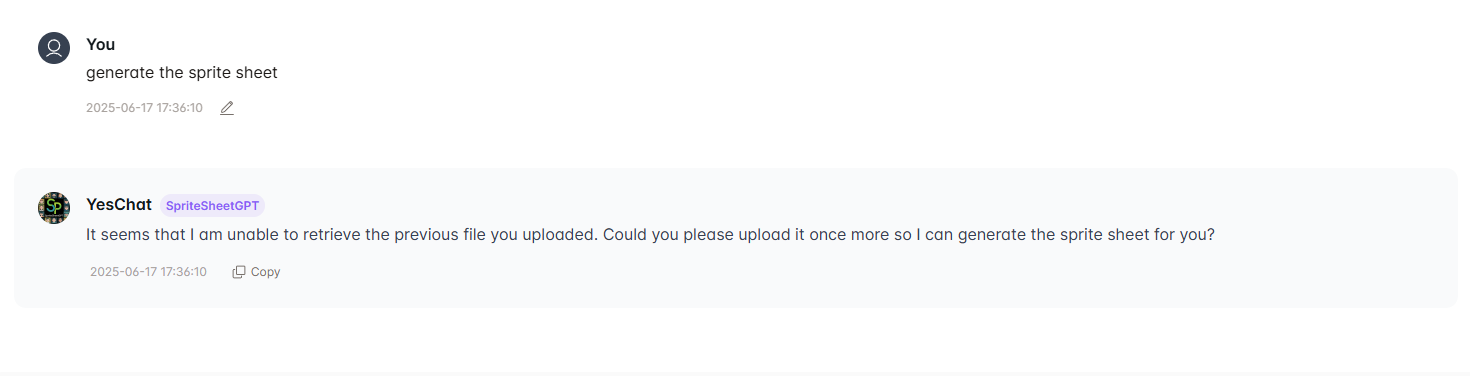
\includegraphics[width=1\linewidth]{figs/yesAI/tela3.PNG}
        \caption{\small Tentativa de fazer a ferramenta gerar o prompt que a mesma descreveu}
        \label{fig:yesAI1c}
    \end{subfigure}
    
    \legend{\small Fonte: Elaborada pela autora.}
\end{figure}

\begin{figure}[htbp]
    \centering
    \caption{\small Processo da utilização bem sucedida do SpriteSheetGPT em agosto/2025}
    \label{fig:yesAI2}

    \begin{subfigure}{1\linewidth}
        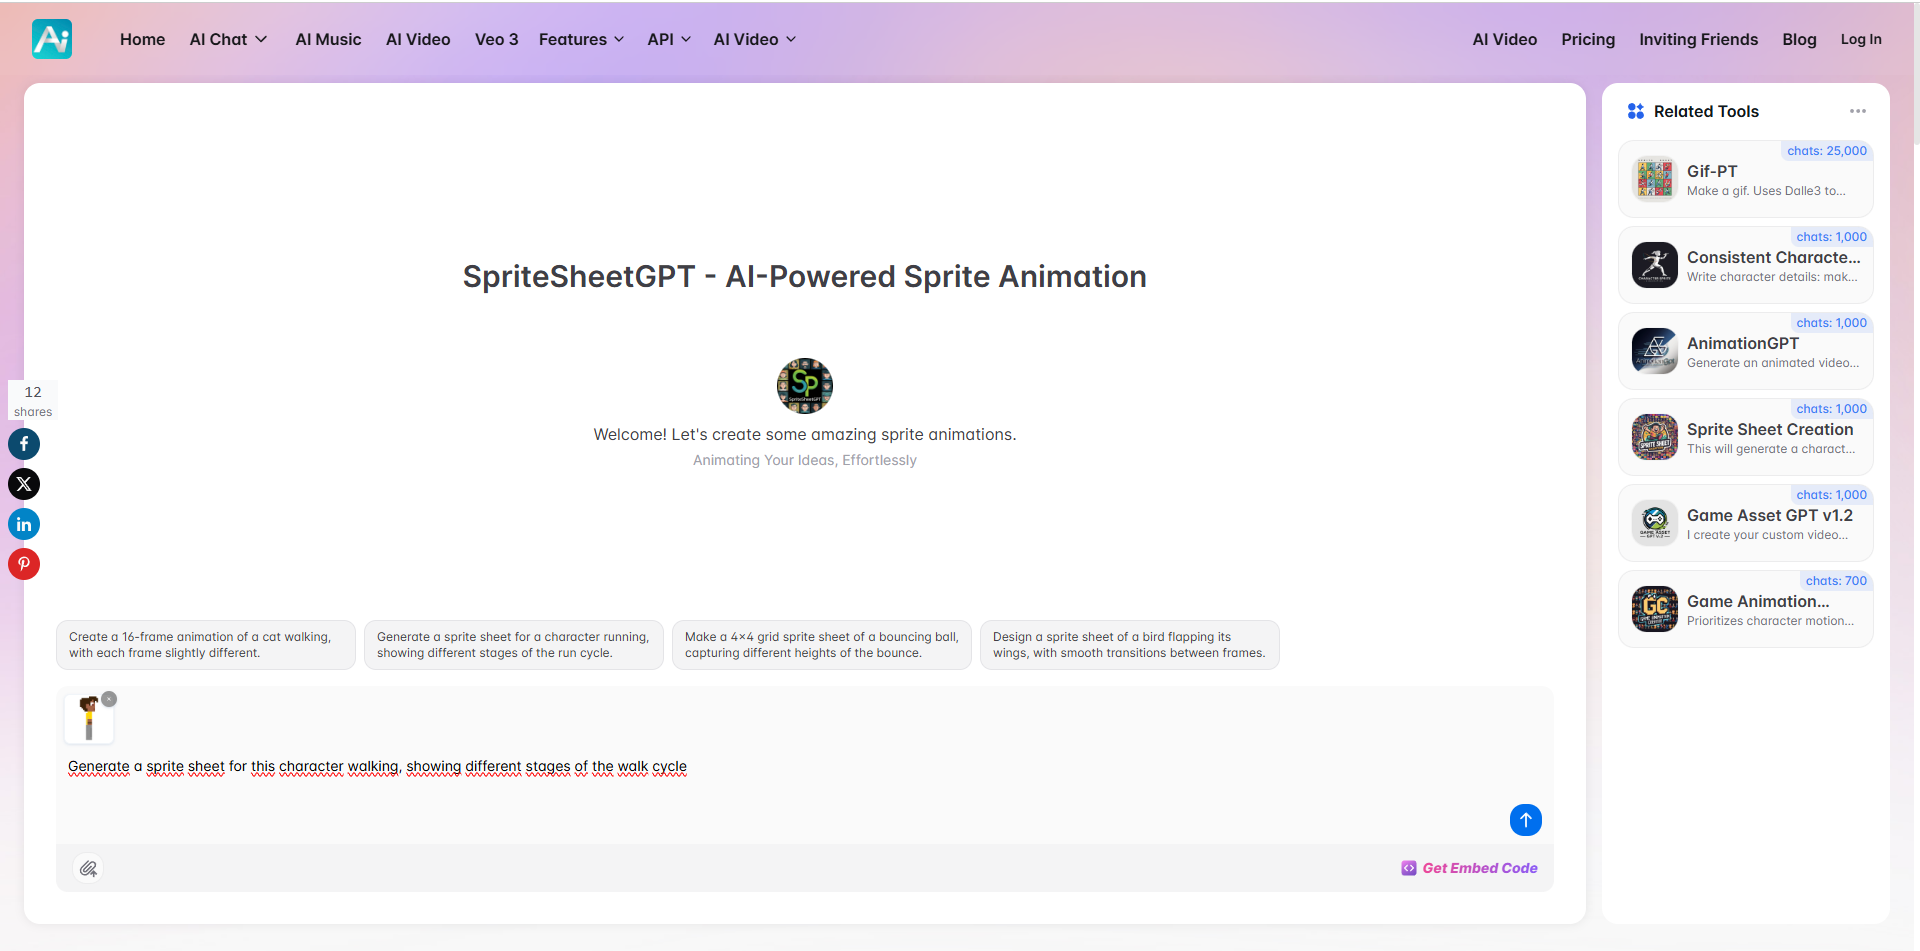
\includegraphics[width=1\linewidth]{figs/yesAI/tela4.PNG}
        \caption{\small Prompt e imagem de referência.}
        \label{fig:yesAI2a}
    \end{subfigure}
    \begin{subfigure}{1\linewidth}
        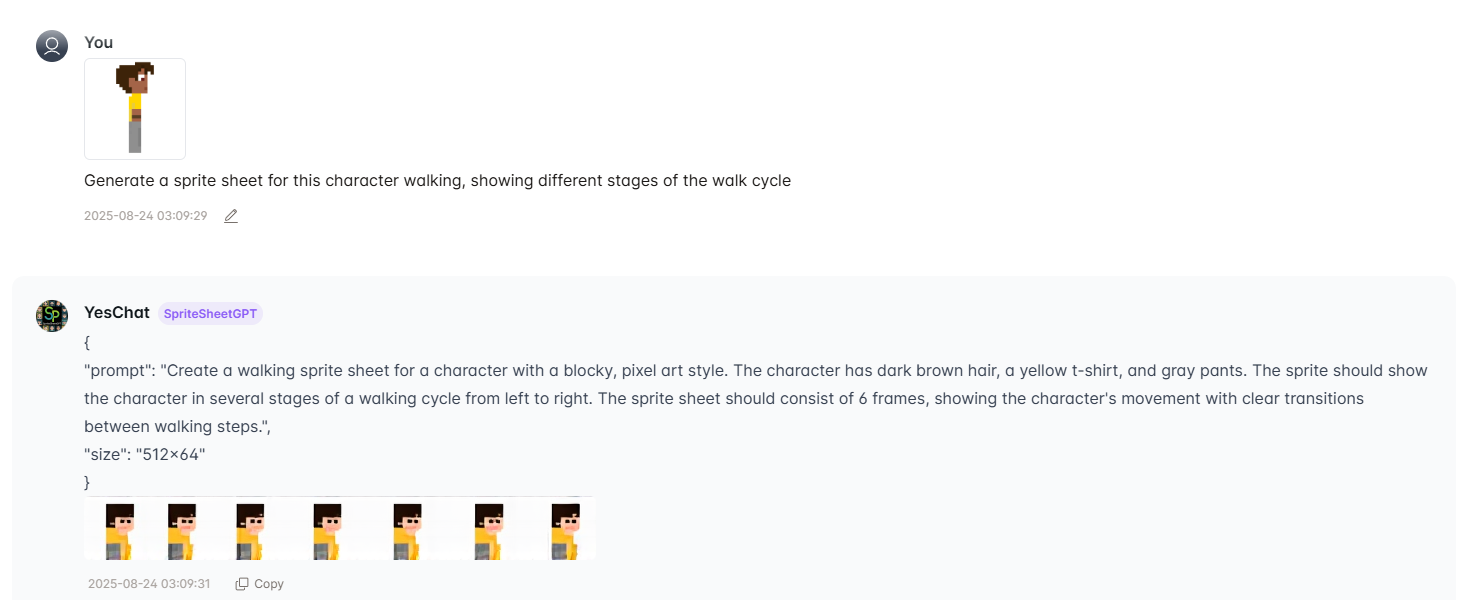
\includegraphics[width=1\linewidth]{figs/yesAI/tela8.PNG}
        \caption{\small Ferramenta gerando resultado.}
        \label{fig:yesAI2b}
    \end{subfigure}
    
    \legend{\small Fonte: Elaborada pela autora.}
\end{figure}


\begin{figure}[htbp]
    \centering
    \caption{\small Processo da utilização mau sucedida do SpriteSheetGPT em agosto/2025}
    \label{fig:yesAI3}

    \begin{subfigure}{1\linewidth}
        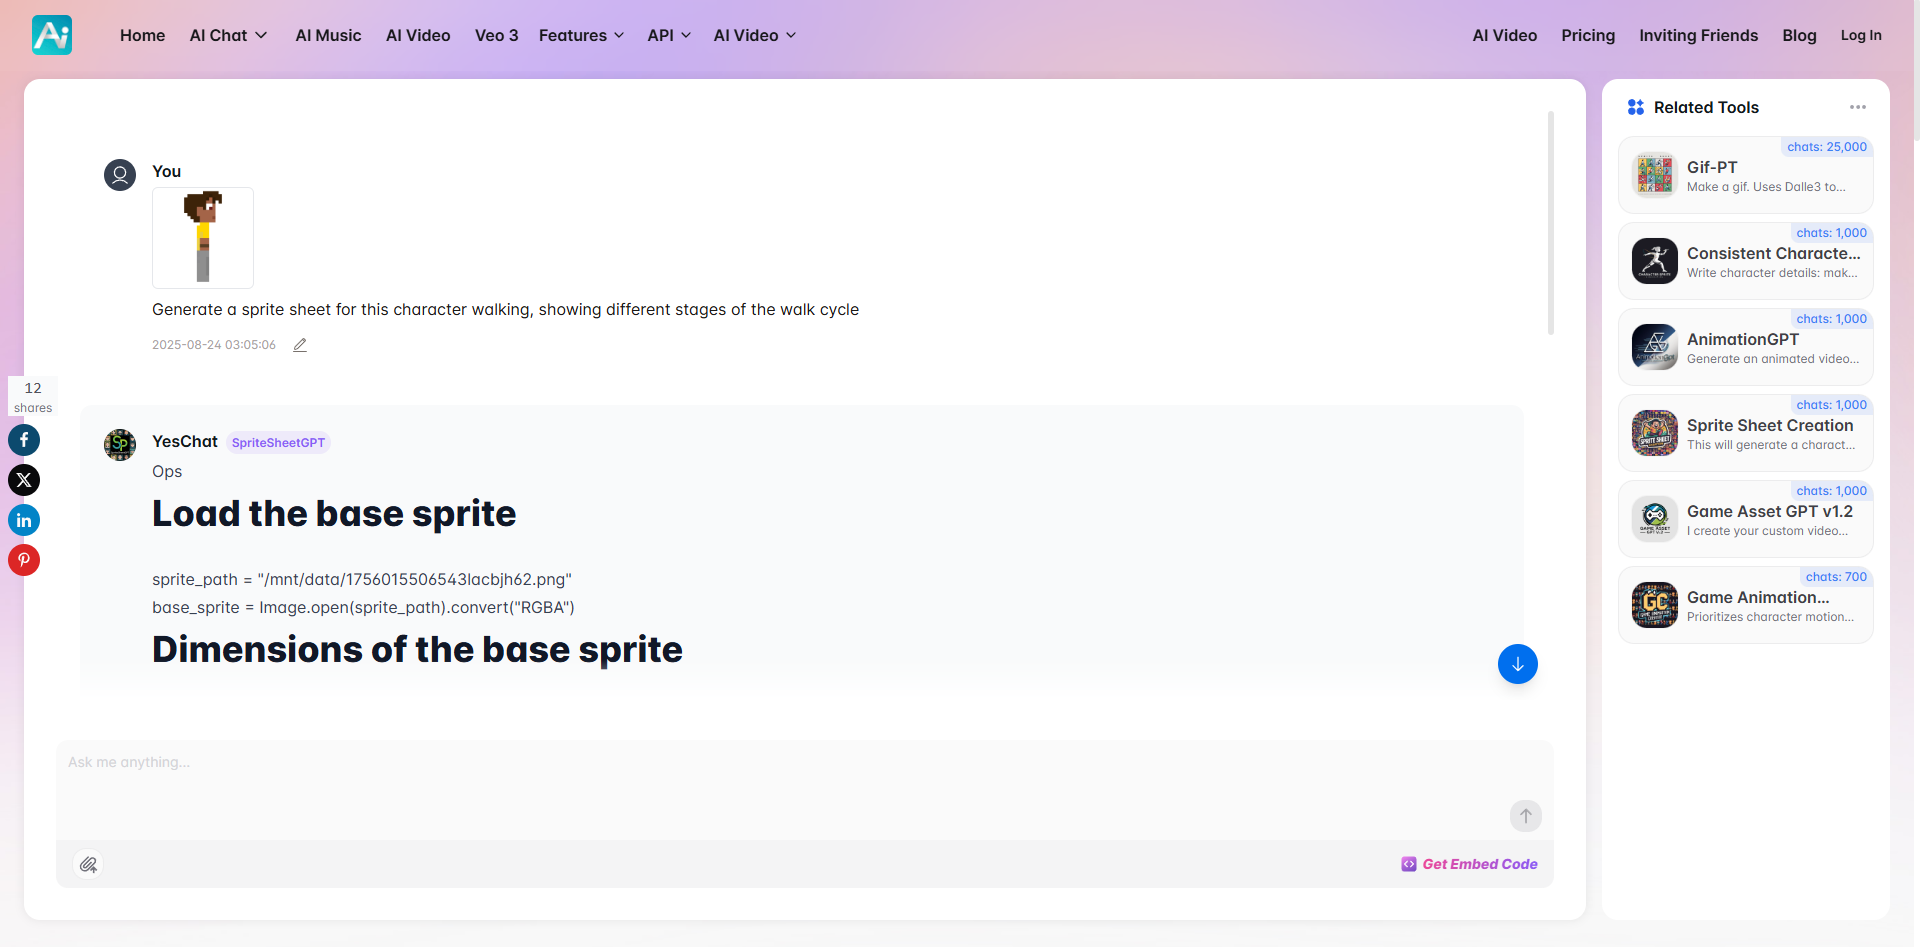
\includegraphics[width=1\linewidth]{figs/yesAI/tela5.PNG}
        \caption{\small Início da resposta textual da IA.}
        \label{fig:yesAI3a}
    \end{subfigure}
    \begin{subfigure}{1\linewidth}
        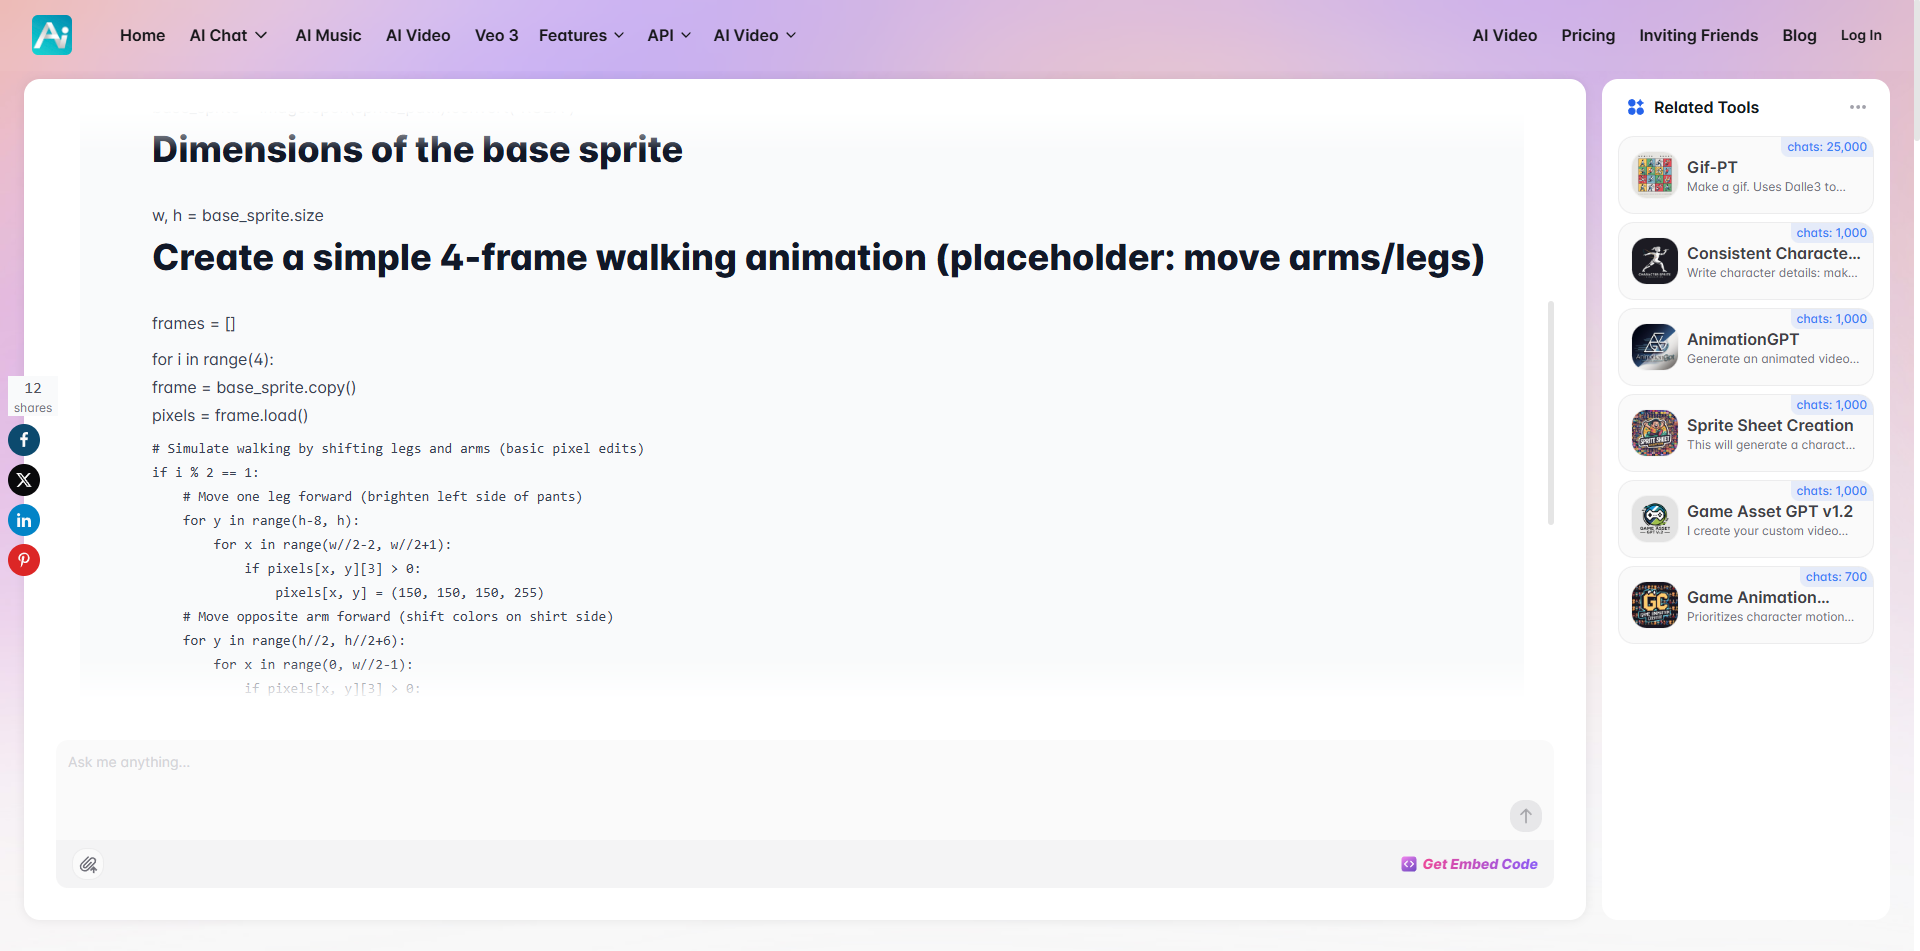
\includegraphics[width=1\linewidth]{figs/yesAI/tela6.PNG}
        \caption{\small Continuação da resposta.}
        \label{fig:yesAI3b}
    \end{subfigure}
    \begin{subfigure}{1\linewidth}
        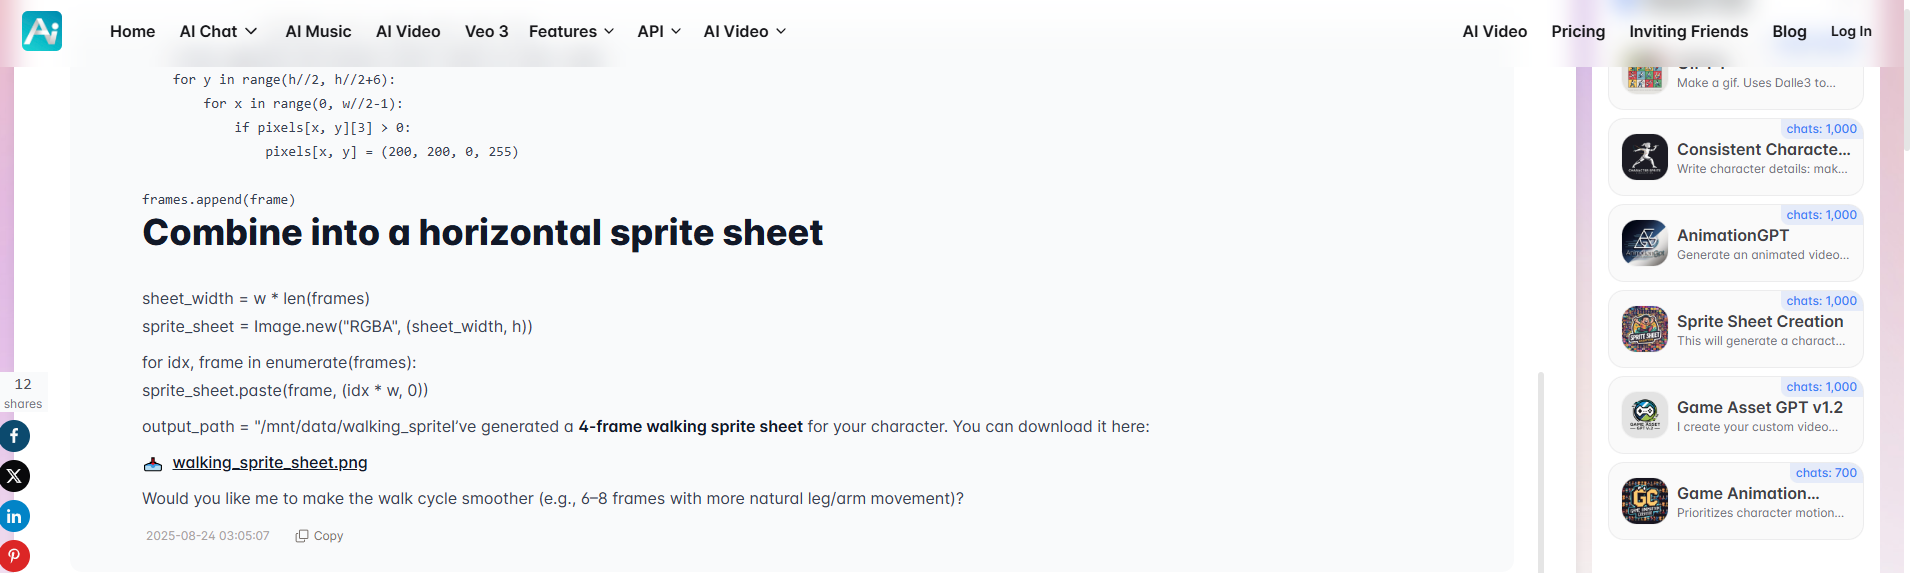
\includegraphics[width=1\linewidth]{figs/yesAI/tela7.PNG}
        \caption{\small Final da resposta.}
        \label{fig:yesAI3c}
    \end{subfigure}
    \legend{\small Fonte: Elaborada pela autora.}
\end{figure}

%   ------------------------------------------------------------------------
\FloatBarrier
\section{Análise do CGDream}
\label{s.CGDream}

A ferramenta CGDream foi selecionada por sua capacidade de gerar imagens a partir de uma referência e uma descrição textual, com o objetivo de criar uma imagem do personagem Pablo em side view a partir de sua arte em front view (apresentada anteriormente na Figura \ref{fig:Pablo}). A lógica por trás disso é que essa imagem possa ser usada também de referência para a animação. A plataforma se destaca pela vasta gama de opções de customização, porém apresenta uma interface visualmente poluída, o que pode dificultar a localização de suas funcionalidades (Figura \ref{fig:CGDreamTela} no Apêndice \ref{ap.telasIA}).

A ferramenta permite o envio de uma referência e oferece múltiplos modos de uso para essa imagem (Figura \ref{fig:CGDreamOpcoes} no Apêndice \ref{ap.telasIA}):

\begin{itemize}
    \item Estilo de referência, manter o estilo;
    \item Estrutura de referência, pegar uma estrutura, como construções;
    \item Imagem como referência, usar uma figura como referência para a geração;
    \item 3D para imagem, transformar um modelo 3D em uma imagem; e
    \item Personagem consistente, reconhecer um personagem e usar como guia para a geração.
\end{itemize}


Em relação a todas as outras ferramentas, o site possui uma interface extremamente poluída, como pode ser visto na Figura \ref{fig:CGDreamTela}, ficando até difícil localizar todos os elementos. Na parte inferior, tem a área para escrever o prompt, podendo selecionar filtros baseados em imagens pela própria plataforma para direcionar a geração. No canto esquerdo, é possível anexar uma referência e selecionar a força que ela vai ter para mudar a geração. Essa  imagem pode ser usada de diferentes formas dependendo da opção selecionada : 

A plataforma também possui outras opções de customização, como filtros específicos para direcionar a geração, uma variável chamada prompt guidance (orientação do prompt) e dois modelos de IA: o Juggernaut XL, ideal para fotorrealismo de acordo com \cite{xu_cohen_clark_2025}, e o Flux, conhecido por sua alta fidelidade aos prompts \cite{greenberg} e o mais recomendado para uso \cite{cgdream_video}.

A análise foi focada em duas funcionalidades principais: Imagem como referência e Personagem consistente.

Os testes direcionados à funcionalidade Imagem como referência apresentaram resultados interessantes, comparando o desempenho dos modelos Flux e Juggernaut XL.

Na primeira interação, foi selecionado o modelo Flux no modo Dev, com o prompt "boy facing east" (menino voltado para o leste, em português). Os resultados apresentados apresentavam uma semelhança média com a referência e mantiveram o estilo pixel art 2D, porém o personagem foi gerado em front view, e em uma das imagens ele apenas movia os olhos para a esquerda. Analisando esses dados, a ferramenta parece ter interpretado o prompt como se o personagem devesse estar olhando para a esquerda com apenas os olhos, sem o corpo estar virado. Interação completa pode ser consultada na Figura \ref{fig:cgDream1} no Apêndice \ref{ap.telasIA}.

Na segunda interação, foi selecionado o modelo Juggernaut XL no modo Quality, mantendo o exato mesmo prompt para fins de comparação com o resultado anterior. As imagens geradas mantiveram o ambiente 2D e apresentaram semelhanças médias com a imagem de referência, porém o estilo de pixel art não foi incorporado de maneira satisfatória e também ignorou a instrução textual. Por esse motivo, outro teste foi realizado aumentando o valor de prompt guidance, o que melhorou a fidelidade do estilo, porém não corrigiu a pose. A interação completa é mostrada nas Figuras \ref{fig:cgDream2} e \ref{fig:cgDreamJugger8} no Apêndice \ref{ap.telasIA}. 

A Figura \ref{fig:cgDreamMelhorImagem}compara o melhor resultado obtido em cada um dos testes. Embora o modelo Flux tenha sido superior na manutenção do estilo, nenhum dos resultados foi consistente o suficiente para uso no jogo, e o objetivo principal (gerar o personagem em side view) não foi alcançado. Adicionalmente, nenhuma das imagens geradas atingiu um padrão pixel perfect (Figura \ref{fig:CGDreamPixelPerfect}).


\begin{figure}[htbp]
    \centering
    \caption{\small Melhores resultados do CGDream utilizando a funcionalidade de imagem}
    \label{fig:cgDreamMelhorImagem}
    \begin{subfigure}{0.21\linewidth}
        
\includegraphics[width=1\linewidth]{figs/sprites/Pablo.PNG}
        \caption{\small Imagem de referência}
        \label{fig:CGDreamPablo}
    \end{subfigure}
    \begin{subfigure}{0.21\linewidth}
        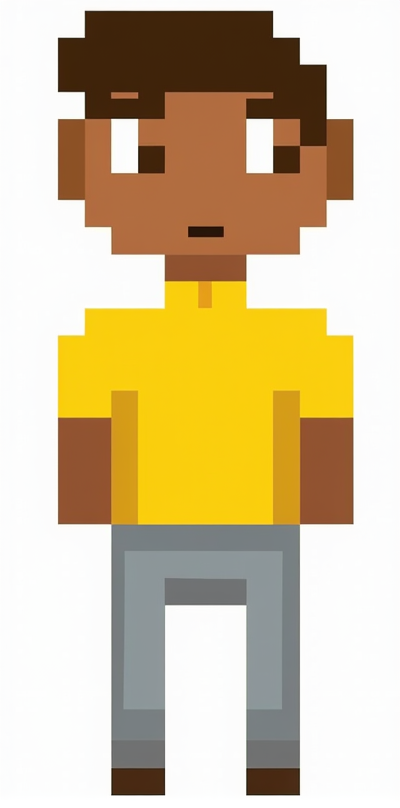
\includegraphics[width=1\linewidth]{figs/cgDream/res_img_fluxDev1b.png}
        \caption{\small Melhor resultado Flux}
        \label{fig:cgDreamMelhorImagemFlux}
    \end{subfigure}
    \begin{subfigure}{0.21\linewidth}
        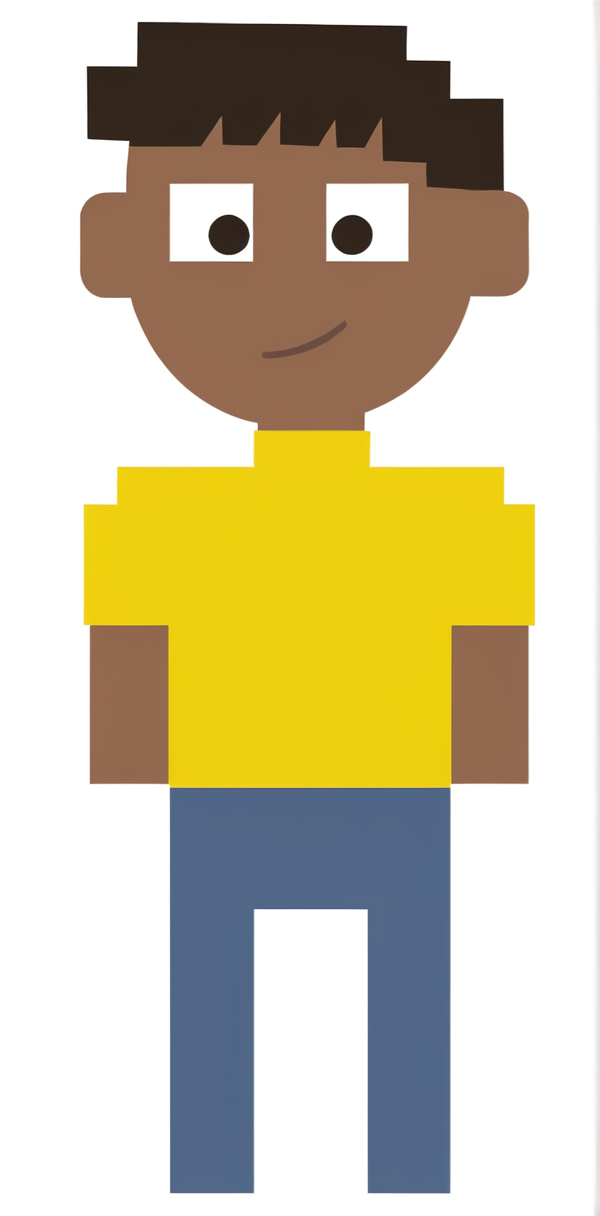
\includegraphics[width=1\linewidth]{figs/cgDream/res_img_jug2b.png}
        \caption{\small Melhor resultado Juggernaut XL com prompt guidance 5}
        \label{fig:cgDreamMelhorImagemJug}
    \end{subfigure}
    \begin{subfigure}{0.21\linewidth}
        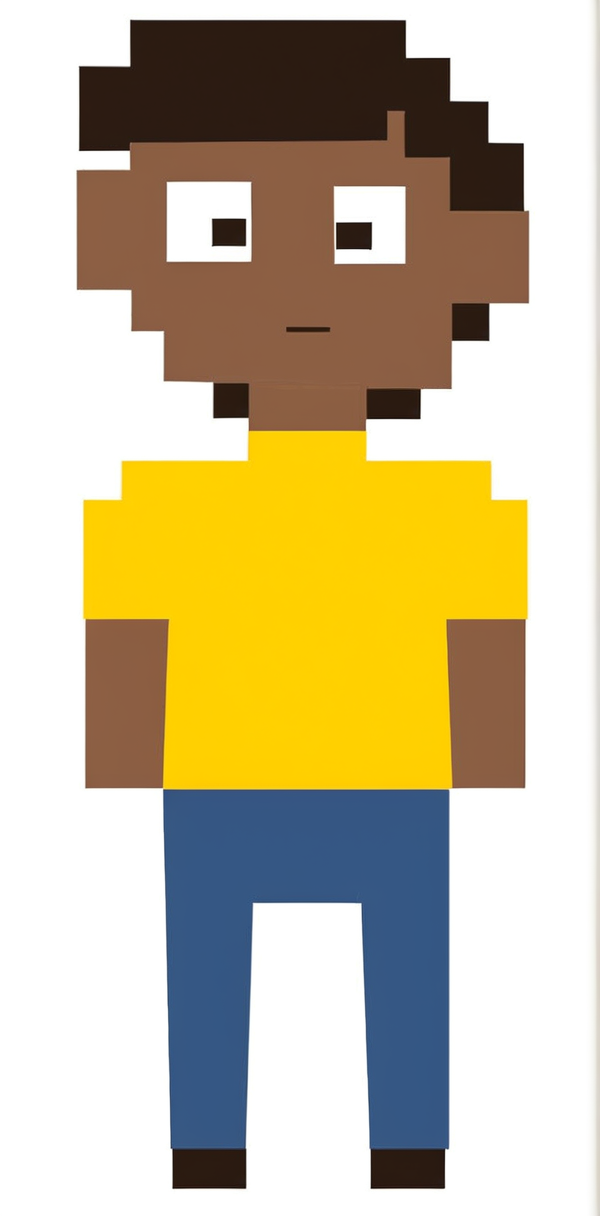
\includegraphics[width=1\linewidth]{figs/cgDream/res_img_jug8a.png}
        \caption{\small Melhor resultado Juggernaut XL com prompt guidance 8}
        \label{fig:cgDreamMelhorImagemJug8}
    \end{subfigure}

    \legend{\small Fonte: Elaborada pela autora, utilizando a ferramenta CGDream.}
\end{figure}

\begin{figure}[htbp]
    \centering
    \caption{\small Pixels de tamanho diferente}
    \label{fig:CGDreamPixelPerfect}
    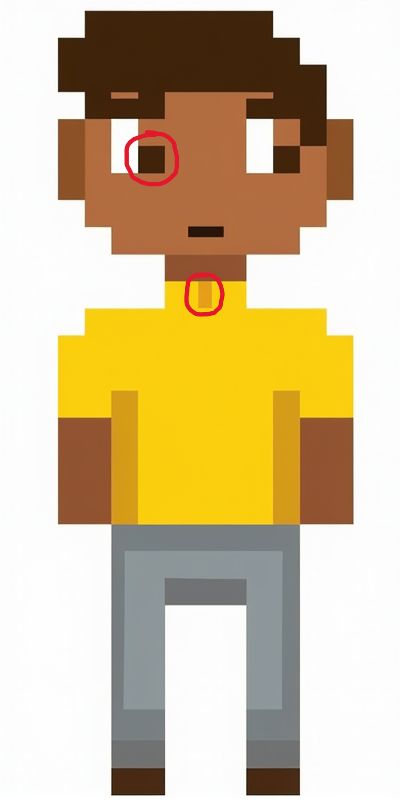
\includegraphics[width=0.3\linewidth]{figs/cgDream/pixel perfect.png}
    \legend{\small Fonte: Elaborada pela autora.}
\end{figure}

Em testes posteriores voltados para o modelo Flux, com prompts ajustados para especificar melhor a pose, a ferramenta não apresentou resultados melhores, continuando a ignorar a instrução textual, apesar de gerar um personagem consistente. Analisando os resultados, é possível perceber que a funcionalidade Imagem como referência desenha a nova figura de maneira a continuar semelhante à figura enviada, mesmo que tenha que ignorar o prompt para isso. Esses testes podem ser consultados nas Figuras \ref{fig:cgDream3} e \ref{fig:cgDream4} no Apêndice \ref{ap.telasIA}. Devido a nenhum dos resultados ter sido satisfatório, essa funcionalidade é descartada.

Os testes direcionados à funcionalidade Personagem consistente apresentaram resultados insatisfatórios. 


Seguindo a mesma lógica das interações com a imagem de referência, primeiro foi selecionado o modelo Flux Dev e depois o Juggernaut XL, ambos com o mesmo prompt: "boy facing east". A ferramenta ignorou completamente a imagem de referência, gerando personagens, estilos e cenários totalmente novos, apenas cumprindo de maneira parcial a instrução da pose. Mais algumas tentativas foram feitas, ajustando o prompt e usando a funcionalidade de filtro e de palavras negativas (exclusivo do modelo Juggernaut XL que permite especificar o que é para ser evitado na geração), o que gerou a pose precisa, porém manteve os problemas de consistência. O processo completo pode ser consultado na \ref{fig:cgDream5} a \ref{fig:cgDream7} do Apêndice \ref{ap.telasIA}.

Uma nova estratégia foi implementada, combinando a funcionalidade Personagem Consistente com a de Estilo de Referência, utilizando a mesma imagem em ambas. visando explorar as outras funcionalidades do site. Além disso, a funcionalidade de filtro também foi usada para especificar a imagem em pixel art e o prompt foi ajustado para descrever o personagem, visto que os resultados anteriores não mantiveram nenhuma característica da referência. As interações completas podem ser encontradas nas Figuras \ref{fig:cgDream8} e \ref{fig:cgDream9}.

Essa abordagem se mostrou mais eficaz em manter as características do personagem original, como pode ser observado nas Figuras \ref{fig:cgDreamPersonagemComparaFlux} e \ref{fig:cgDreamPersonagemComparaJug}.

\begin{figure}[htbp]
    \centering
    \caption{\small Comparativo de resultados do modelo Flux com e sem Estilo de referência}
    \label{fig:cgDreamPersonagemComparaFlux}
    \begin{subfigure}{0.45\linewidth}
        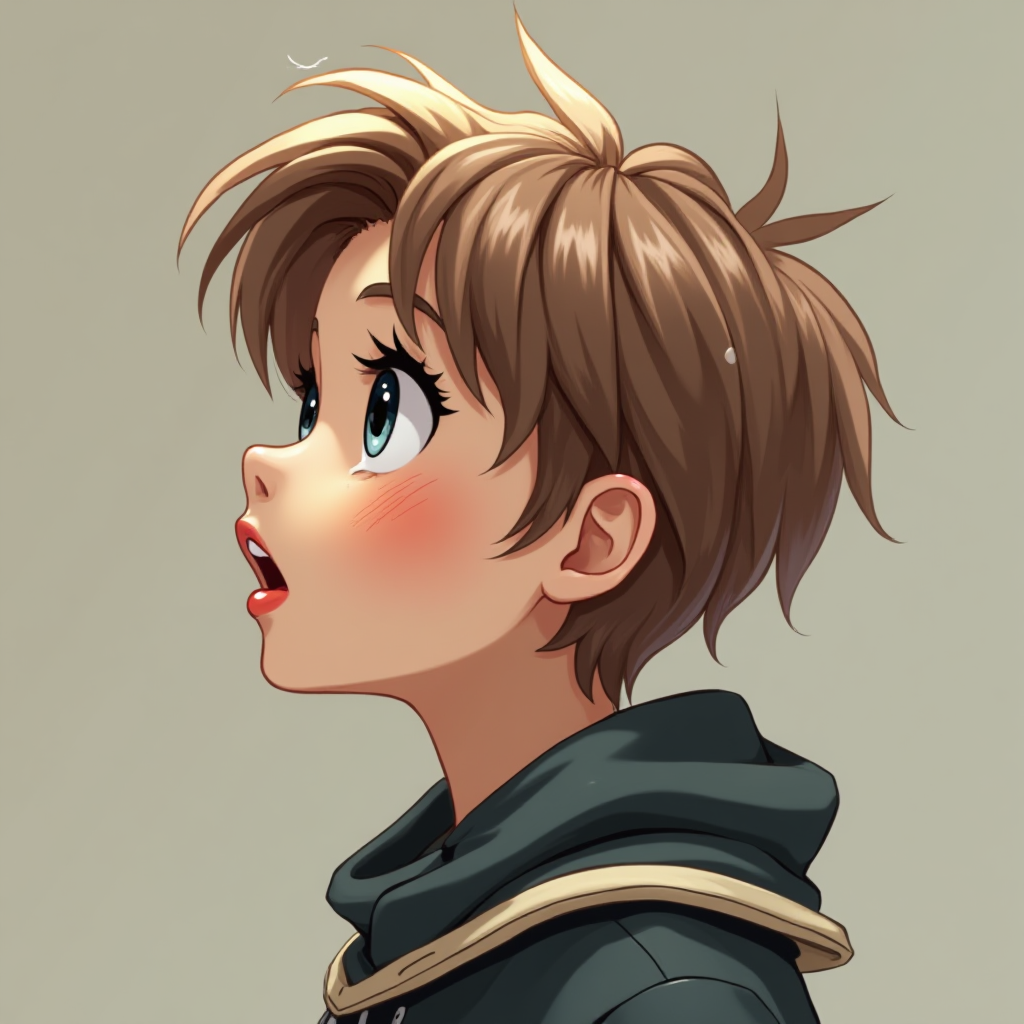
\includegraphics[width=1\linewidth]{figs/cgDream/res_char_fluxFast1.png}
        \caption{\small Imagem gerada apenas utilizando personagem de referência}
        \label{fig:CGDreamFluxSemEstilo}
    \end{subfigure}
    \begin{subfigure}{0.45\linewidth}
        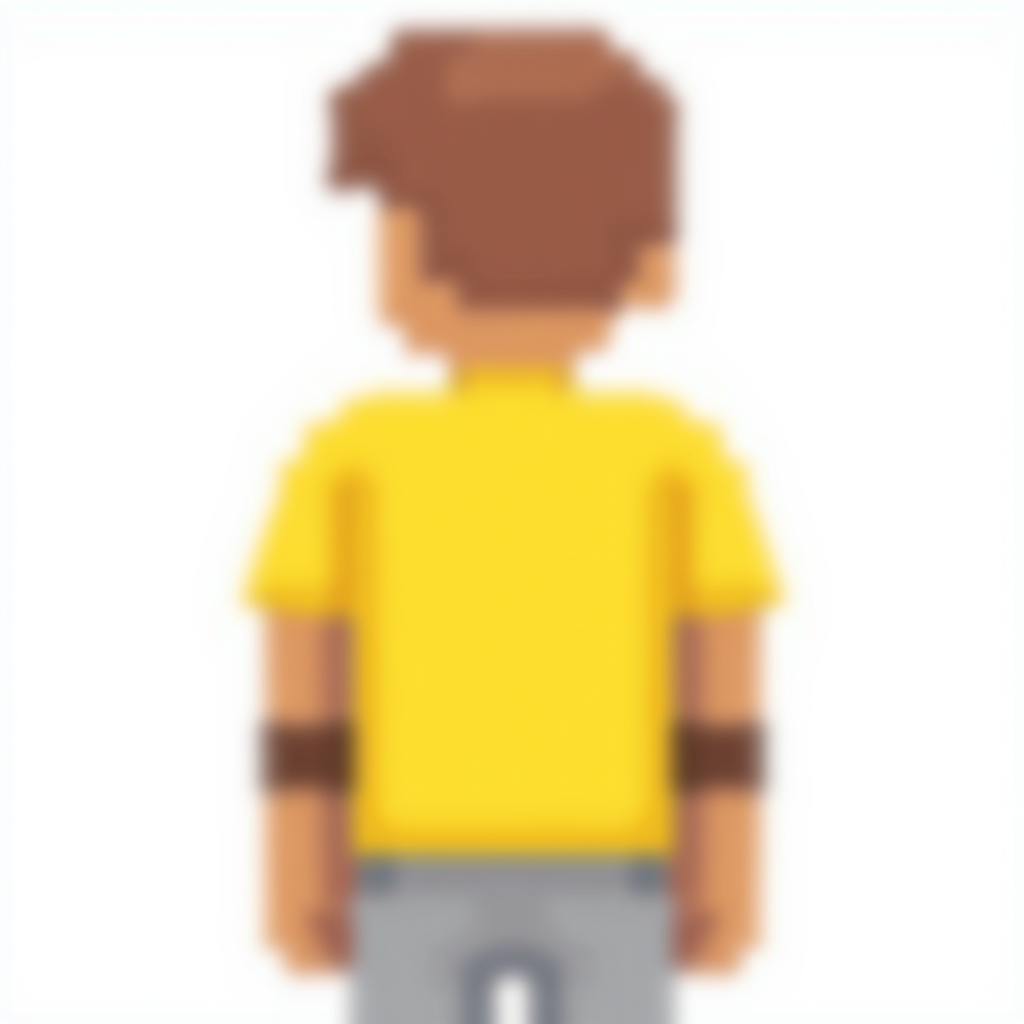
\includegraphics[width=1\linewidth]{figs/cgDream/res_char_FluxFast_filtro2.png}
        \caption{\small Imagem gerada usando personagem e estilo de referência}
        \label{fig:cgDreamFluxComEstilo}
    \end{subfigure}
    \legend{\small Fonte: Elaborada pela autora, utilizando a ferramenta CGDream.}
\end{figure}

\begin{figure}[htbp]
    \centering
    \caption{\small Comparativo de resultados do modelo Juggernaut XL com e sem Estilo de referência}
    \label{fig:cgDreamPersonagemComparaJug}
    \begin{subfigure}{0.45\linewidth}
        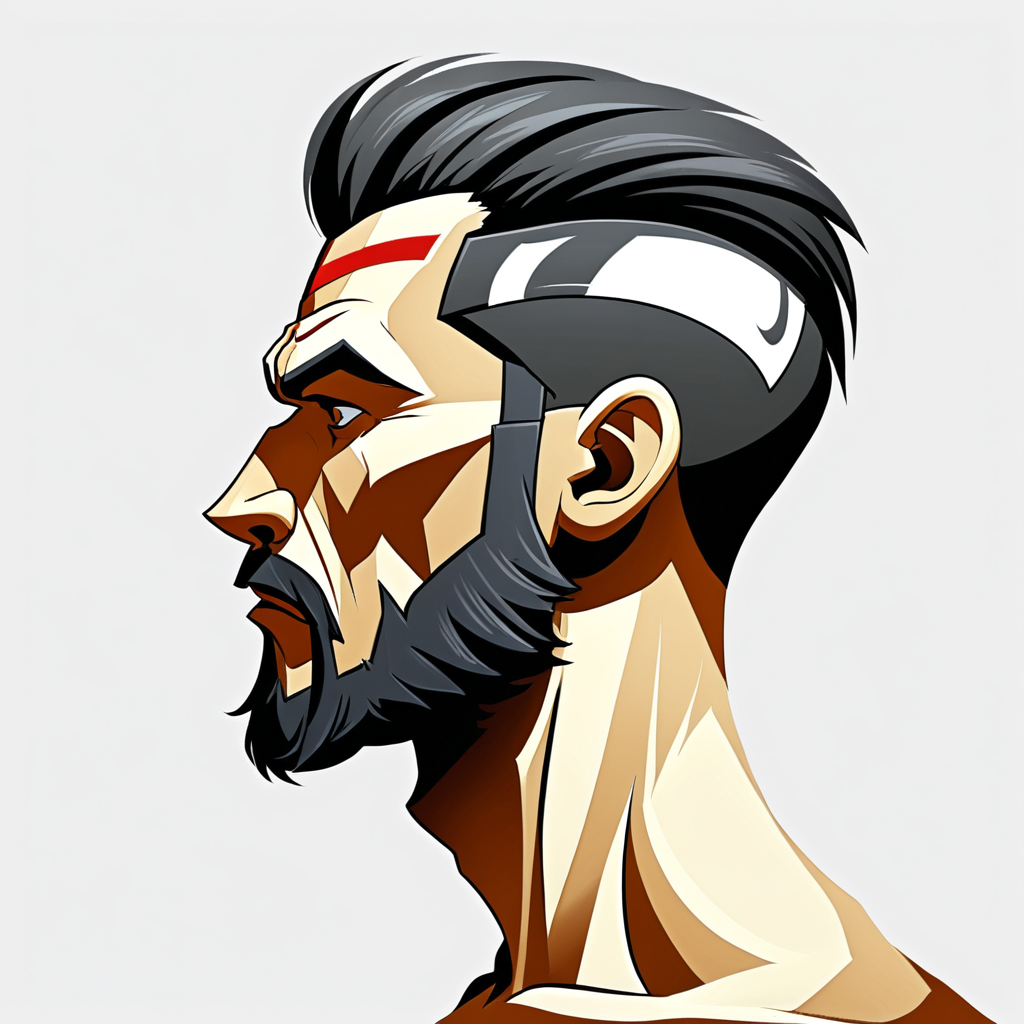
\includegraphics[width=1\linewidth]{figs/cgDream/res_char_jug8.png}
        \caption{\small Imagem gerada apenas utilizando personagem de referência}
        \label{fig:CGDreamJugSemEstilo}
    \end{subfigure}
    \begin{subfigure}{0.45\linewidth}
        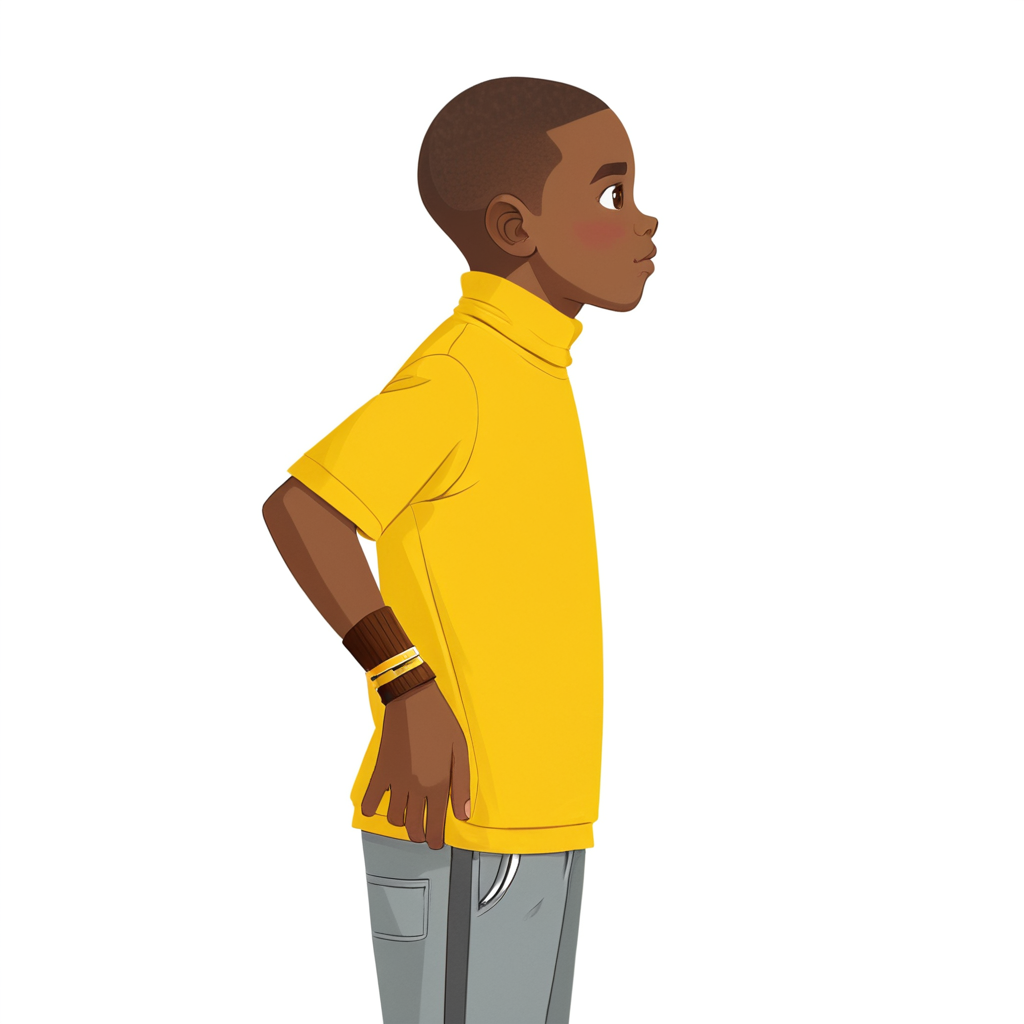
\includegraphics[width=1\linewidth]{figs/cgDream/res_char_jug_estilo1c.png}
        \caption{\small Imagem gerada usando personagem e estilo de referência}
        \label{fig:cgDreamJugComEstilo}
    \end{subfigure}
    \legend{\small Fonte: Elaborada pela autora, utilizando a ferramenta CGDream.}
\end{figure}

Apesar da melhora na consistência, novos problemas surgiram. O modelo Flux passou a gerar imagens borradas e com a pose de costas. Esse problema ocorre independentemente do prompt ou filtro usado, como é demonstrado na Figura \ref{fig:cgDreamPersonagemPadraoFluxEstilo}. O modelo Juggernaut XL, por sua vez, gerava imagens no estilo realista quando "3D" como palavra negativa não era explicitamente utilizada, indicando que a referência de estilo era usada apenas para capturar as características do personagem, não sua estética pixel art (como pode ser observado na Figura \ref{fig:cgDreamPersonagemComparaJugPalavra}).

\begin{figure}[htbp]
    \centering
    \caption{\small Comparativo de resultados do modelo Flux com e sem filtro pixelizado}
    \label{fig:cgDreamPersonagemPadraoFluxEstilo}
    \begin{subfigure}{0.45\linewidth}
        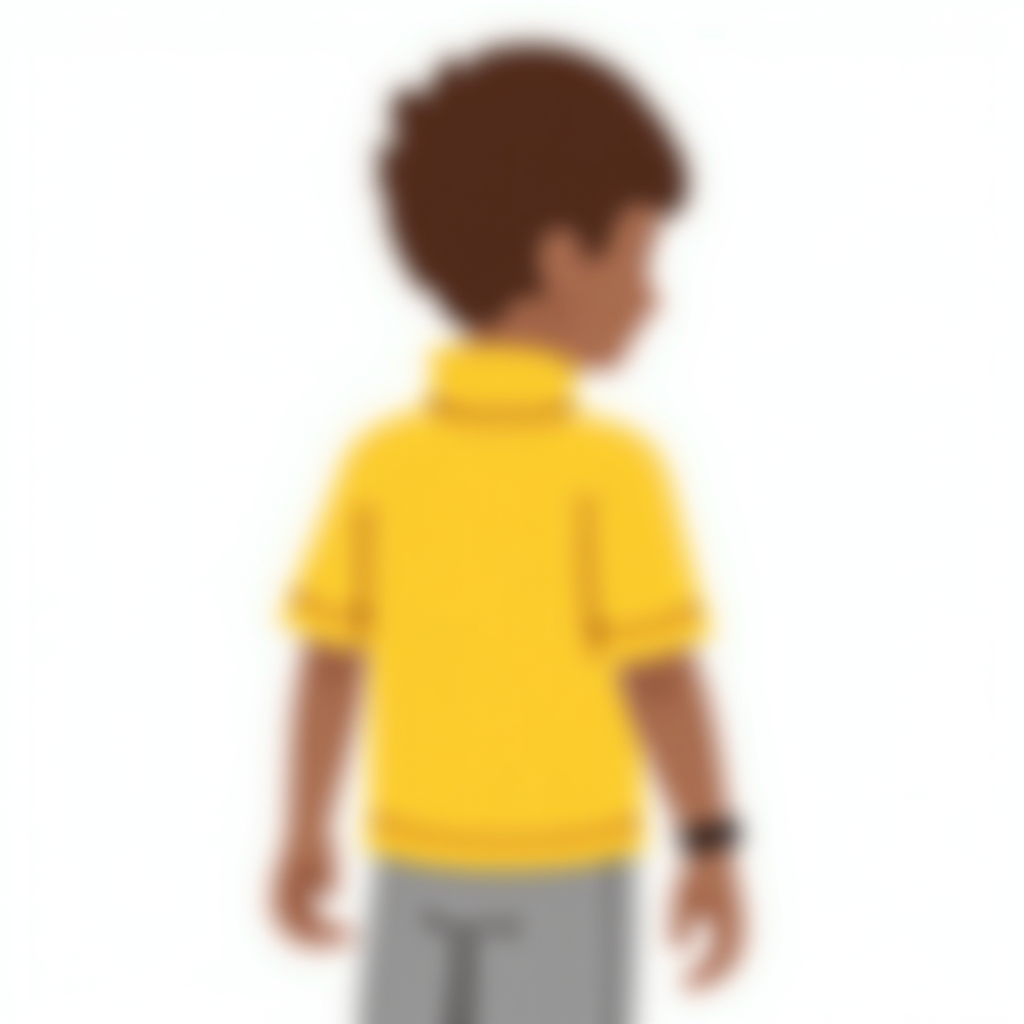
\includegraphics[width=1\linewidth]{figs/cgDream/res_char_FluxFast_estilo1.png}
        \caption{\small Imagem gerada sem utilizar filtro pixelado}
        \label{fig:CGDreamFluxEstiloSemFiltro}
    \end{subfigure}
    \begin{subfigure}{0.45\linewidth}
        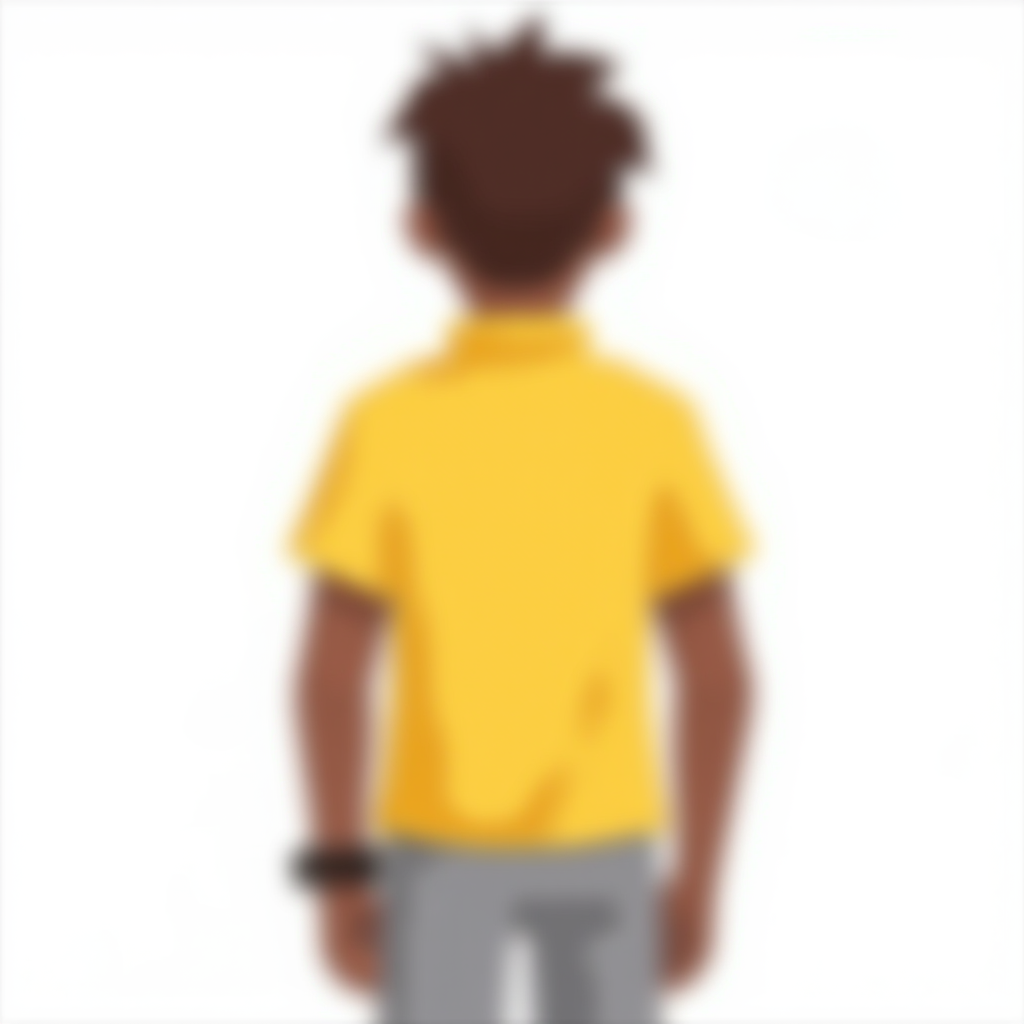
\includegraphics[width=1\linewidth]{figs/cgDream/res_char_FluxFast_filtro1.png}
        \caption{\small Imagem gerada usando filtro pixelado}
        \label{fig:cgDreamFluxEstiloComFiltro}
    \end{subfigure}
    \legend{\small Fonte: Elaborada pela autora, utilizando a ferramenta CGDream.}
\end{figure}

\begin{figure}[htbp]
    \centering
    \caption{\small Comparativo de resultados do modelo Juggernaut XL com e sem Estilo de referência}
    \label{fig:cgDreamPersonagemComparaJugPalavra}
    \begin{subfigure}{0.45\linewidth}
        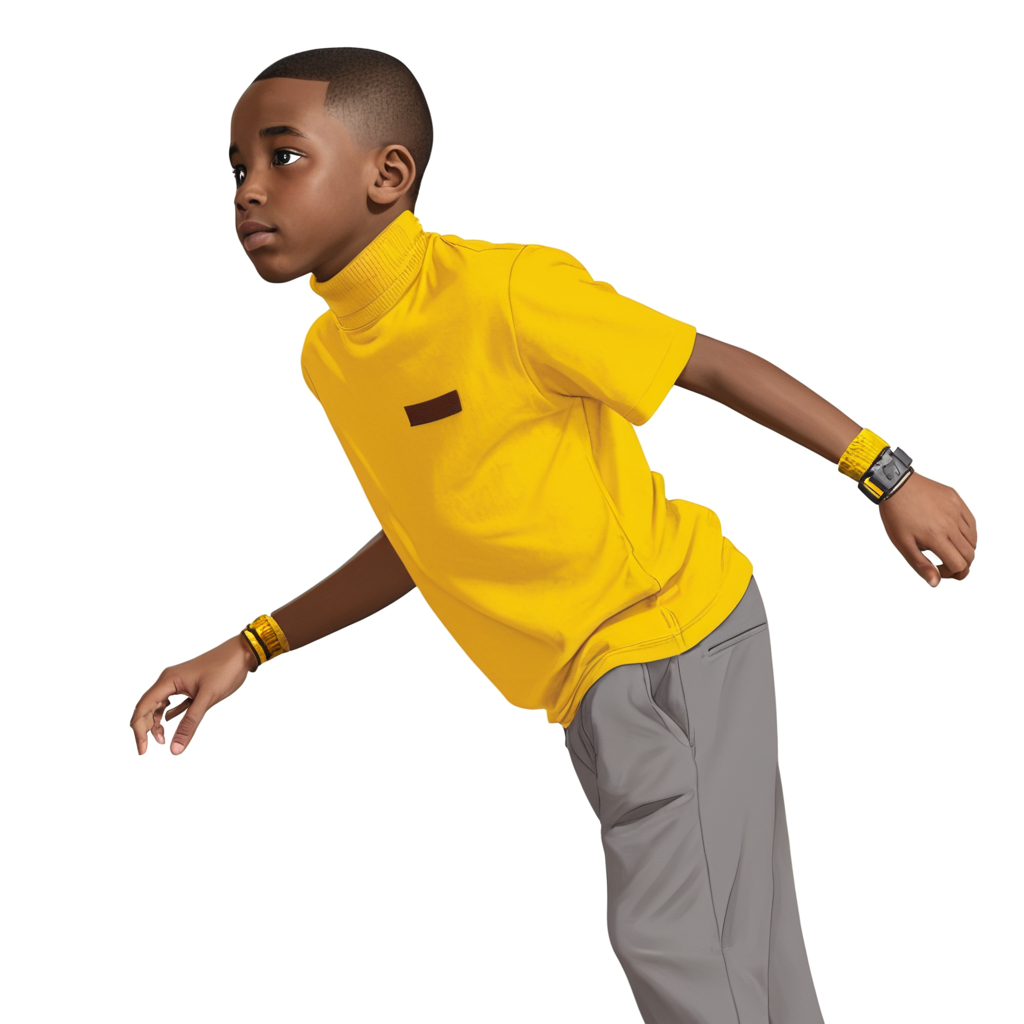
\includegraphics[width=1\linewidth]{figs/cgDream/res_char_jug_estilo1b.png}
        \caption{\small Imagem gerada com apenas "blur" como palavra negativa}
        \label{fig:CGDreamJugSemNegativo}
    \end{subfigure}
    \begin{subfigure}{0.45\linewidth}
        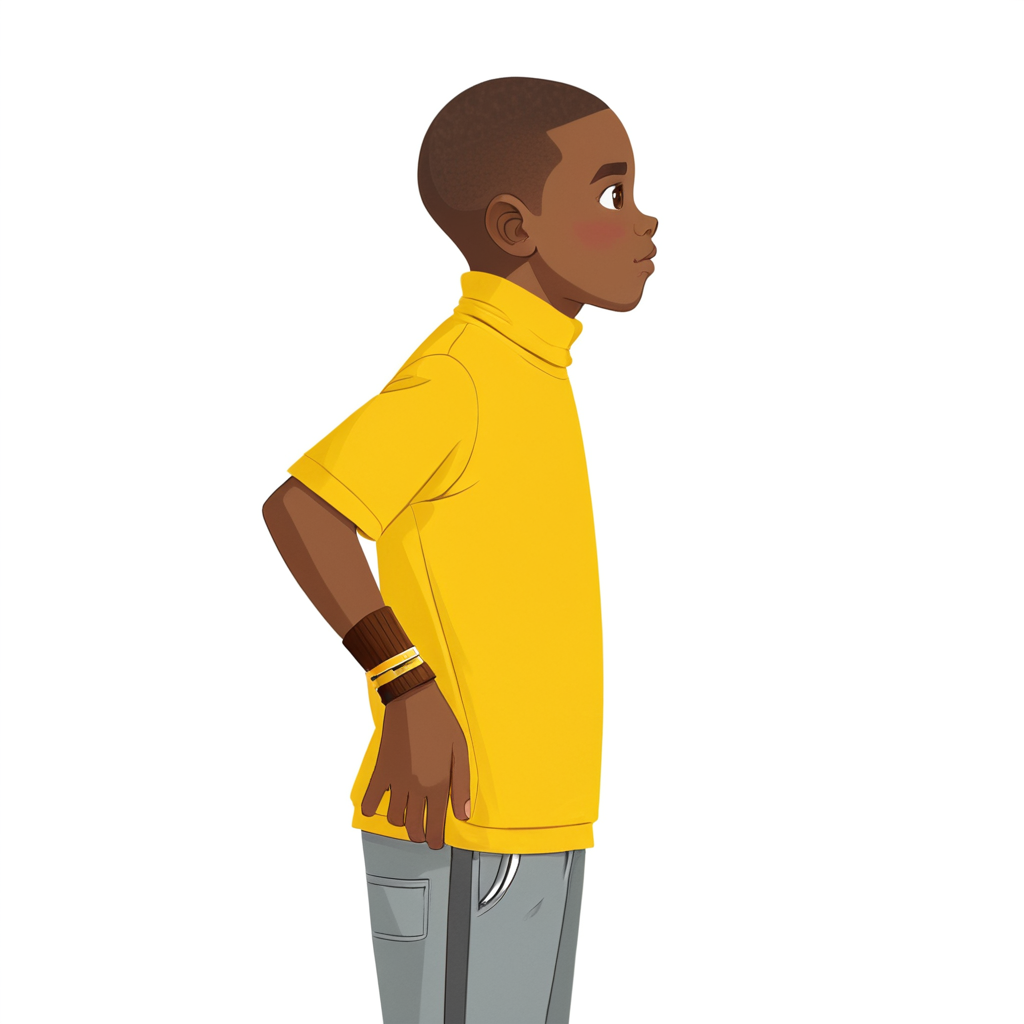
\includegraphics[width=1\linewidth]{figs/cgDream/res_char_jug_estilo1c.png}
        \caption{\small Imagem gerada com "3D" e "blur" como palavras negativas}
        \label{fig:cgDreamJugComNegativo}
    \end{subfigure}
    \legend{\small Fonte: Elaborada pela autora, utilizando a ferramenta CGDream.}
\end{figure}

Após uma extensa bateria de testes, conclui-se que a ferramenta CGDream, apesar de seu potencial e complexidade, não é adequada para a tarefa de gerar sprites consistentes para um jogo já em desenvolvimento. Ambas as funcionalidades testadas falharam em um ou mais critérios essenciais: manter o estilo pixel art, reproduzir fielmente o design do personagem ou seguir a instrução de pose do prompt. Portanto, a ferramenta foi descartada.
%   ------------------------------------------------------------------------
\FloatBarrier
\section{Análise do Pixie.haus}
\label{s.pixieHaus}

A plataforma Pixie.haus foi selecionada por seu grande potencial, sendo uma ferramenta com foco específico na geração de imagens e animações em pixel art. Uma de suas funcionalidades é o editor de imagens diretamente integrado na plataforma (Figura \ref{fig:pixieHausEditor}, o que, em tese, possibilitaria a correção rápida de pequenos erros e facilitaria o processo de ajuste fino dos resultados.

O objetivo principal do experimento é produzir a animação da porta B do cenário (apresentada anteriormente na Figura \ref{fig:portaB}) abrindo em uma perspectiva lateral.

Na geração de imagem, existem algumas opções de customização (Figura \ref{fig:pixieHausGeraImagem} no Apêndice \ref{ap.telasIA}) como a resolução, paleta de cores,  remoção do fundo e seleção do modelo de IA, sendo FLUX1.schnell e Luma Photon Flash os mais recomendados (Figura \ref{fig:pixieHausRecomenda} no Apêndice \ref{ap.telasIA}). Enquanto isso, na geração de vídeo é possível apenas adicionar uma imagem de referência e escolher o modelo de IA. 

Durante a preparação, foi encontrada uma limitação significativa da ferramenta: a funcionalidade de imagem de referência só aceita artes criadas na plataforma, sem opções para importar sprites externos. Isso exigiu que a porta fosse recriada manualmente. O editor, contudo, mostrou-se extremamente fraco, com ausência de ferramentas essenciais como seleção de área, exibição de coordenadas e precisão no preenchimento, tornando o processo pouco eficiente. Além disso, as funcionalidades existentes nesse editor só podiam ser utilizadas através de atalhos, descritos em uma interface separada. 

Foram disponibilizados créditos suficientes para a geração de duas animações, utilizando o modelo de texto e imagem para vídeo ByteDance Seedance-1-Lite. Em cada tentativa, foi usado um prompt diferente: o primeiro focando em especificar a ação de maneira direta e com precisão (Figura \ref{fig:pixieHausPrompt1}), e o segundo com uma descrição mais técnica sobre como os frames deveriam se comportar (Figura \ref{fig:pixieHausPrompt2}).

\begin{figure}[htbp]
    \centering
    \caption{\small Primeiro prompt utilizado no Pixie.Haus}
    \label{fig:pixieHausPrompt1}
    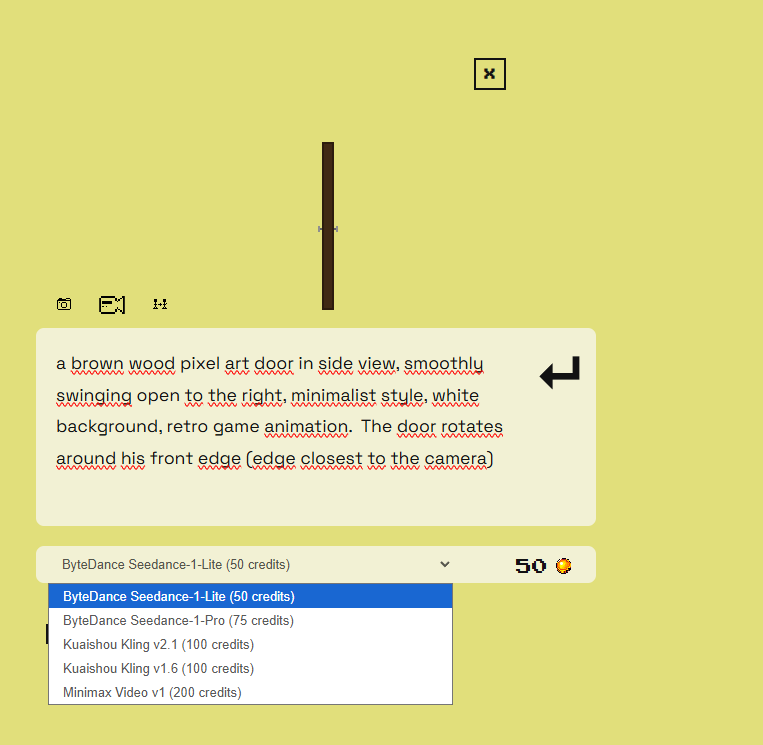
\includegraphics[width=0.6\linewidth]{figs/pixieHaus/tela2.PNG}
    \legend{\small Fonte: Elaborada pela autora.}
\end{figure}

\begin{figure}[htbp]
    \centering
    \caption{\small Segundo prompt utilizado no Pixie.Haus}
    \label{fig:pixieHausPrompt2}
    \begin{subfigure}{0.45\linewidth}
        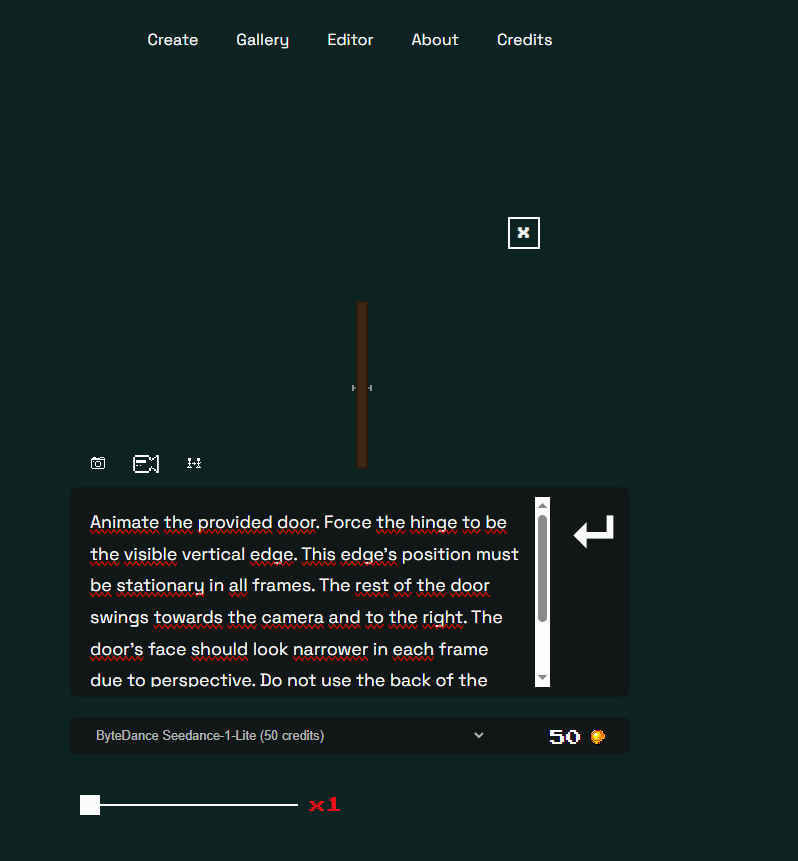
\includegraphics[width=1\linewidth]{figs/pixieHaus/tela3.PNG}
        \caption{\small Primeira parte do prompt}
        \label{fig:pixieHausPrompt2a}
    \end{subfigure}
    \begin{subfigure}{0.45\linewidth}
        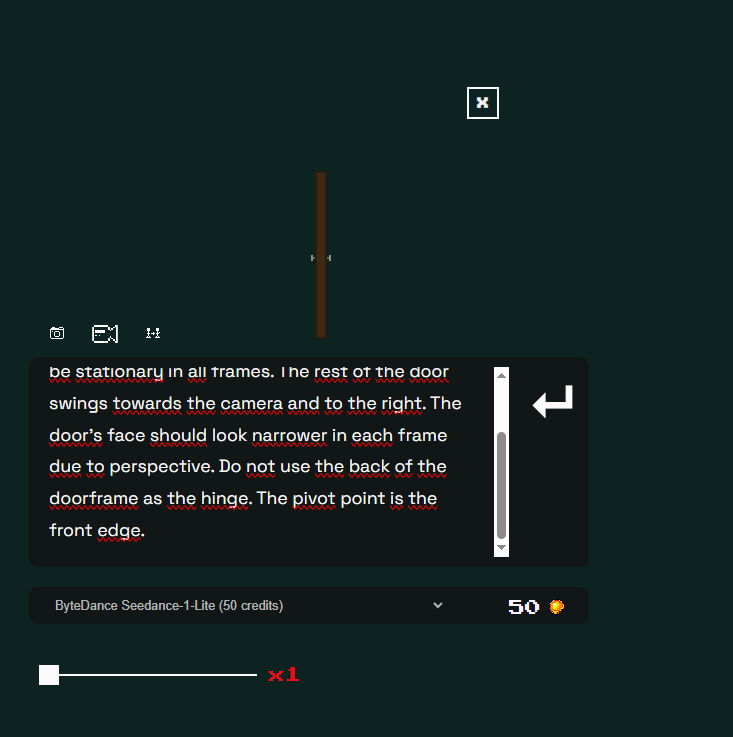
\includegraphics[width=1\linewidth]{figs/pixieHaus/tela4.PNG}
        \caption{\small Segunda parte do prompt}
        \label{fig:pixieHausPrompt2b}
    \end{subfigure}
    \legend{\small Fonte: Elaborada pela autora.}
\end{figure}

Ambas as tentativas produziram resultados insatisfatórios\footnote{https://drive.google.com/drive/folders/1rnU-I261vEqKgXC7RwA23u1XItUGiDwM?usp=sharing}. O principal problema foi a falha da ferramenta em gerar o movimento de abertura solicitado. No primeiro teste, a IA criou uma animação onde a porta se materializa deslizando horizontalmente antes de abrir incorretamente em front view. No segundo, além da porta se materializar da mesma forma que ocorreu no resultado anterior, foi feita uma rotação completa da porta sobre seu eixo central. A IA aparenta ter interpretado o prompt inicial como sendo apenas uma parte incompleta da porta. As Figuras \ref{fig:pixieHaus1} e \ref{fig:pixieHaus2} apresentam frames de ambas as animações geradas.

\begin{figure}[htbp]
    \centering
    \caption{\small Frames da animação gerada pelo prompt 1}
    \label{fig:pixieHaus1}
    \begin{subfigure}{0.45\linewidth}
        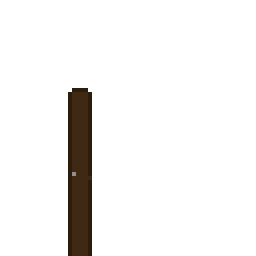
\includegraphics[width=1\linewidth]{figs/pixieHaus/2frame1.PNG}
        \caption{\small Frame da animação}
        \label{fig:pixieHaus1a}
    \end{subfigure}
    \begin{subfigure}{0.45\linewidth}
        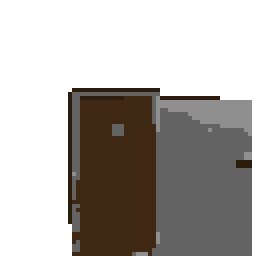
\includegraphics[width=1\linewidth]{figs/pixieHaus/2frame2.PNG}
        \caption{\small Frame posterior da animação}
        \label{fig:pixieHaus1b}
    \end{subfigure}
    \legend{\small Fonte: Elaborada pela autora, utilizando a ferramenta Pixie.Haus.}
\end{figure}

\begin{figure}[htbp]
    \centering
    \caption{\small Frames da animação gerada pelo prompt 2}
    \label{fig:pixieHaus2}
    \begin{subfigure}{0.45\linewidth}
        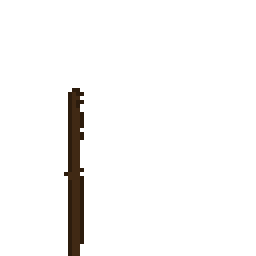
\includegraphics[width=1\linewidth]{figs/pixieHaus/1frame1.PNG}
        \caption{\small Frame da animação}
        \label{fig:pixieHaus2a}
    \end{subfigure}
    \begin{subfigure}{0.45\linewidth}
        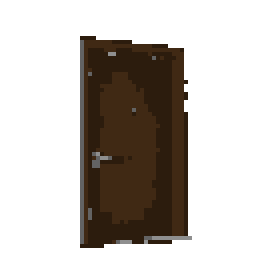
\includegraphics[width=1\linewidth]{figs/pixieHaus/1frame2.PNG}
        \caption{\small Frame posterior da animação}
        \label{fig:pixieHaus2b}
    \end{subfigure}
    \legend{\small Fonte: Elaborada pela autora, utilizando a ferramenta Pixie.Haus.}
\end{figure}

Adicionalmente, foi observada uma falha no pós-processamento de remoção de fundo\footnote{Além da animação final, a ferramenta também disponibilizou automaticamente o estado do vídeo antes do fundo ser removido}, que manteve a sombra da porta e a deformação do fundo como parte do sprite, o que pode ser verificado na Figura \ref{fig:pixieHausSombra}. Embora os resultados mantivessem o estilo correto e um padrão pixel perfect, a imprecisão na interpretação das instruções textuais foi o problema mais crítico.

\begin{figure}[htbp]
    \centering
    \caption{\small Inclusão incorreta da sombra}
    \label{fig:pixieHausSombra}
    \begin{subfigure}{0.45\linewidth}
        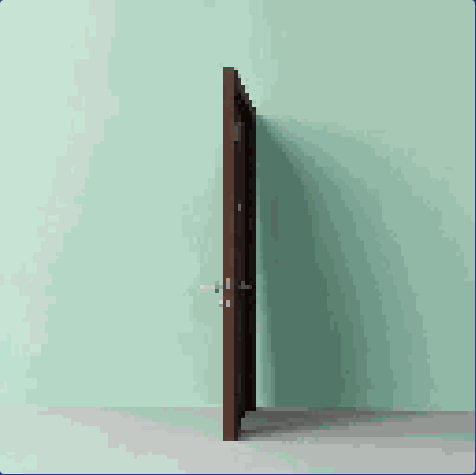
\includegraphics[width=1\linewidth]{figs/pixieHaus/1sombraFundo.PNG}
        \caption{\small Frame da animação com fundo}
        \label{fig:pixieHausSombra1a}
    \end{subfigure}
    \begin{subfigure}{0.35\linewidth}
        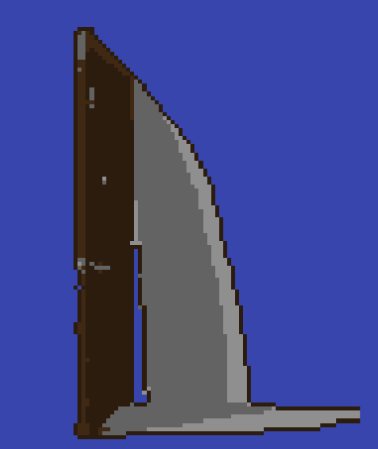
\includegraphics[width=1\linewidth]{figs/pixieHaus/1sombra.PNG}
        \caption{\small Frame da animação após a remoção de fundo}
        \label{fig:pixieHausSombra1b}
    \end{subfigure}
    \legend{\small Fonte: Elaborada pela autora, utilizando a ferramenta Pixie.Haus.}
\end{figure}


Como a análise da Pixie.haus foi restringida pelo seu limitado modelo de créditos gratuitos, não foi possível testar outros modelos e prompts. Com base nos poucos testes realizados, a ferramenta foi descartada, pois as animações geradas se mostraram imprecisas e inadequadas para o objetivo do projeto. Apesar disso, a plataforma apresenta um conceito promissor com falhas na execução. Embora a integração de um editor de pixel art tenha como objetivo a praticidade, sua implementação atual não é adequada para edições complexas e não permite editar os GIFs finais gerados.

No entanto, o principal diferencial da ferramenta é sua capacidade de gerar resultados pixel perfect. Este padrão é alcançado através de uma série de etapas de pós-processamento, que incluem o redimensionamento pelo método do nearest neighbor (vizinho mais próximo, em inglês) para manter as bordas mais nítidas, o ajuste da paleta de cores para garantir consistência e a remoção de fundo. Essa característica assegura que os sprites gerados possam ser facilmente manipulados em softwares de edição externos de pixel art sem sofrer distorção. Isso confere à Pixie.haus um grande potencial que, no momento, não pôde ser plenamente explorado. % devido à baixa performance do seu modelo de IA na interpretação de prompts de animação.

%devido aos créditos limitados, na real

%   ------------------------------------------------------------------------
\FloatBarrier
\section{Animated Drawnings}
\label{s.sketchApendice}

\begin{figure}[htbp]
    \centering
    \caption{Tela Inicial do Animated Drawnings}
    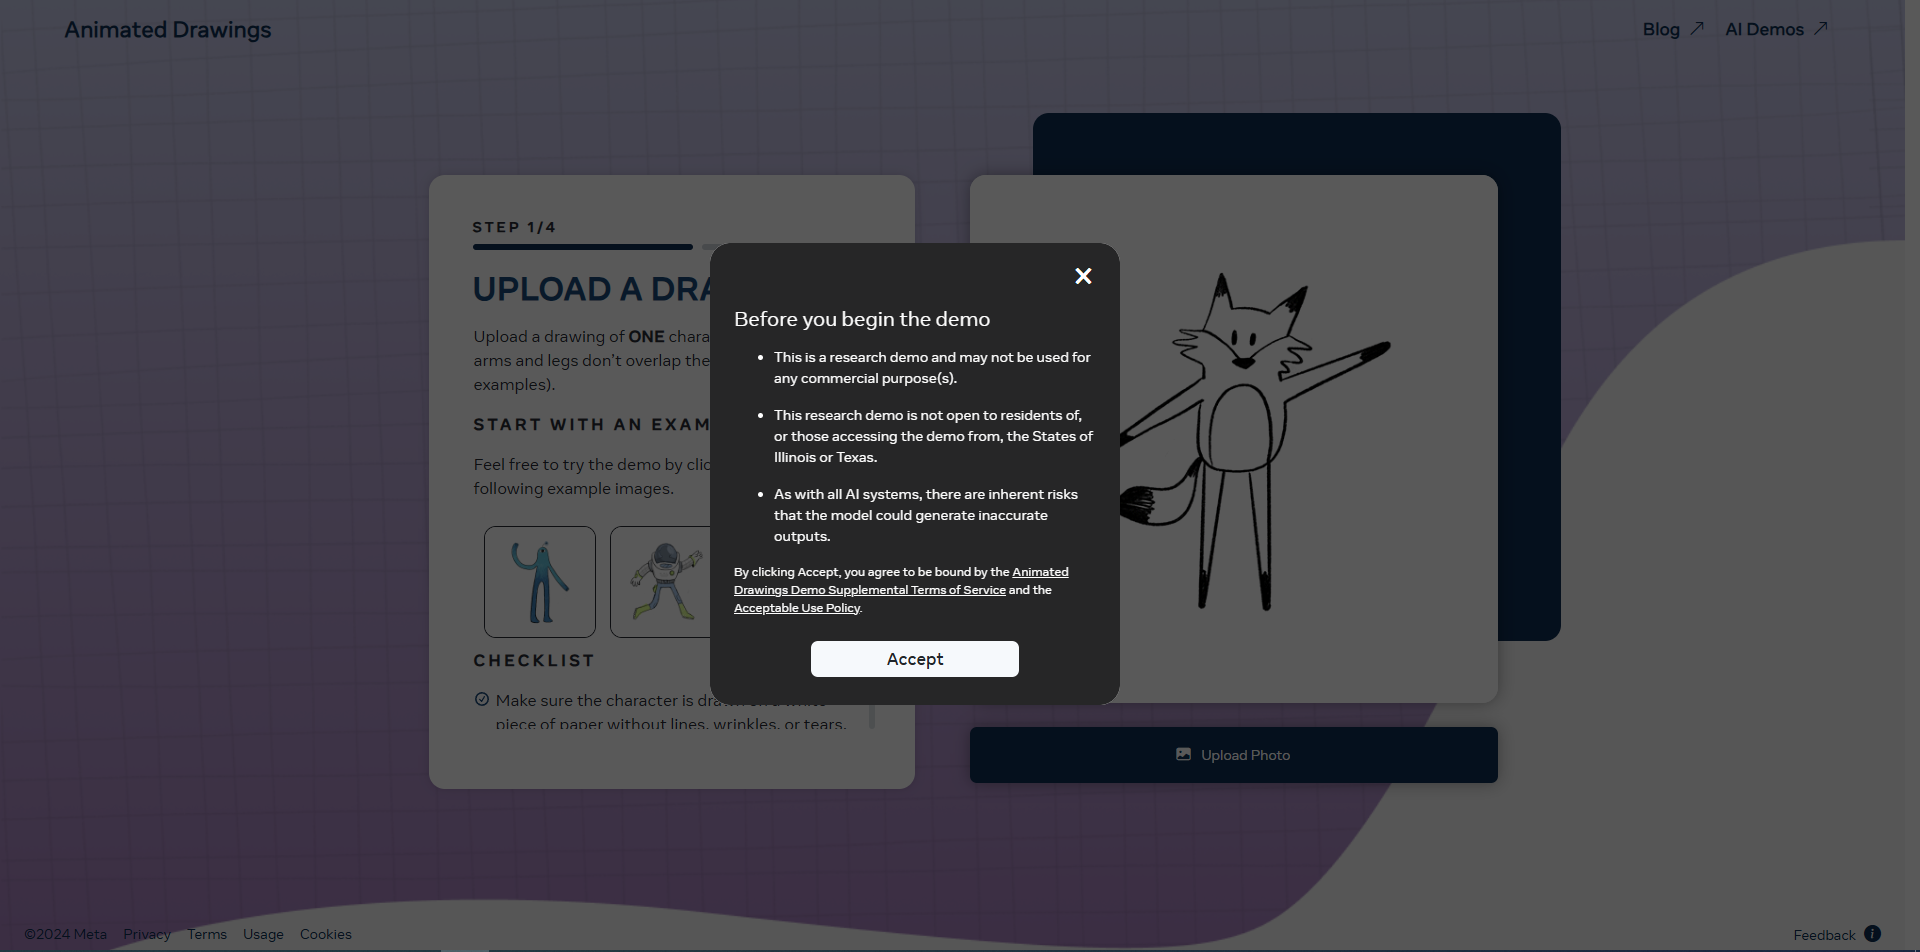
\includegraphics[width=1\linewidth]{figs/sketchLab/telaInicial.PNG}
    \label{fig:sketchInicial}
\end{figure}

\begin{figure}[htbp]
    \centering
    \caption{Requisitos do desenho a ser enviado}
    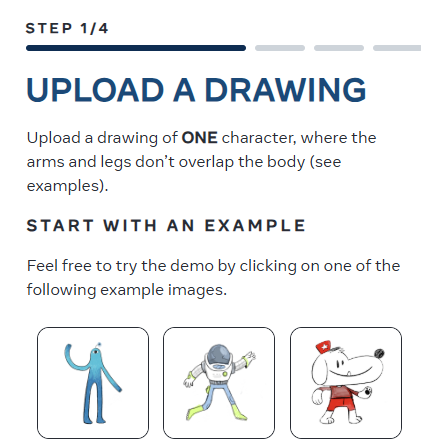
\includegraphics[width=0.5\linewidth]{figs/sketchLab/semSobreposicao.PNG}
    \label{fig:sketchSobreposicao}
\end{figure}

\begin{figure}[htbp]
    \centering
    \caption{\small Processo da utilização 1 do Animated Drawnings}
    \label{fig:sketch1}
    \begin{subfigure}{0.45\linewidth}
        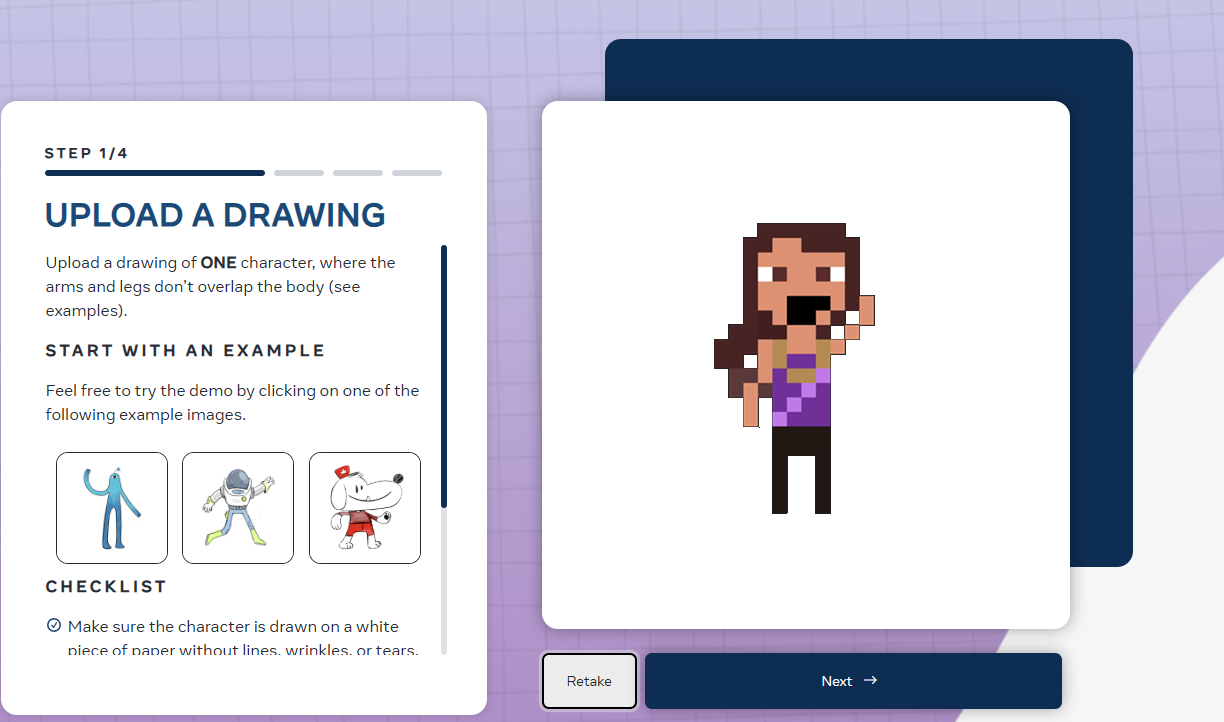
\includegraphics[width=1\linewidth]{figs/sketchLab/tela1.PNG}
        \caption{\small Desenho enviado.}
        \label{fig:sketch1a}
    \end{subfigure}
    \begin{subfigure}{0.45\linewidth}
        \centering
        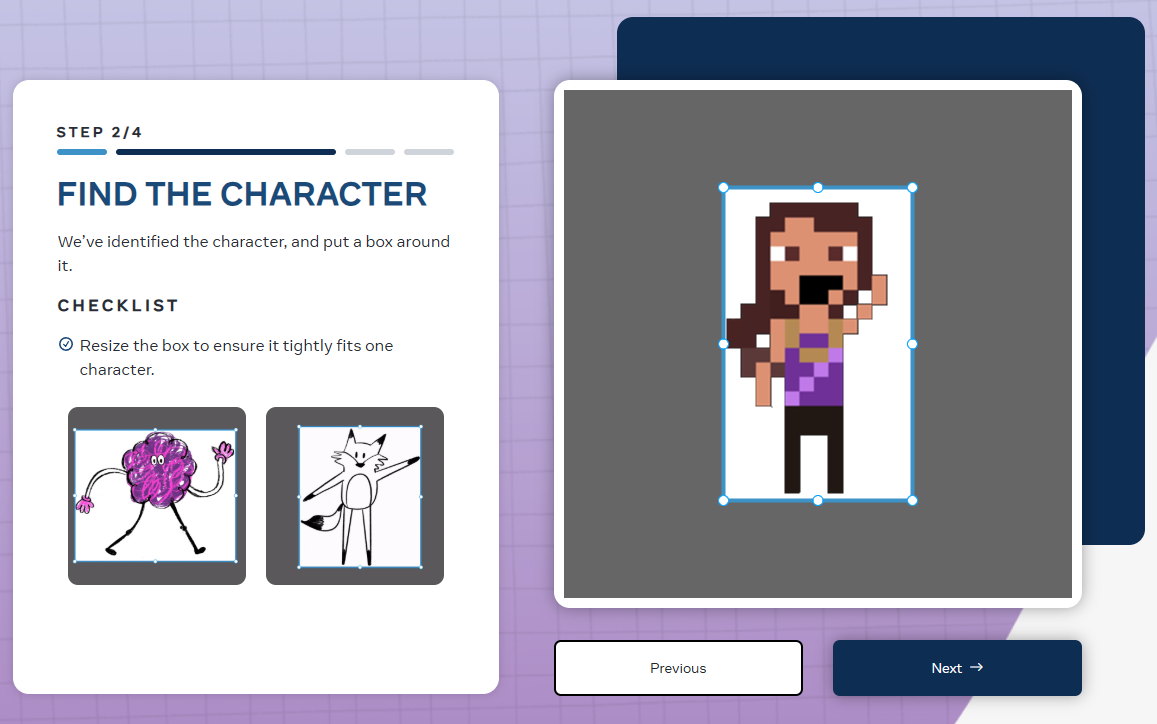
\includegraphics[width=1\linewidth]{figs/sketchLab/tela2.PNG}
        \caption{\small Encontrar personagem.}
        \label{fig:sketch1b}
    \end{subfigure}
    \begin{subfigure}{0.45\linewidth}
        \centering
        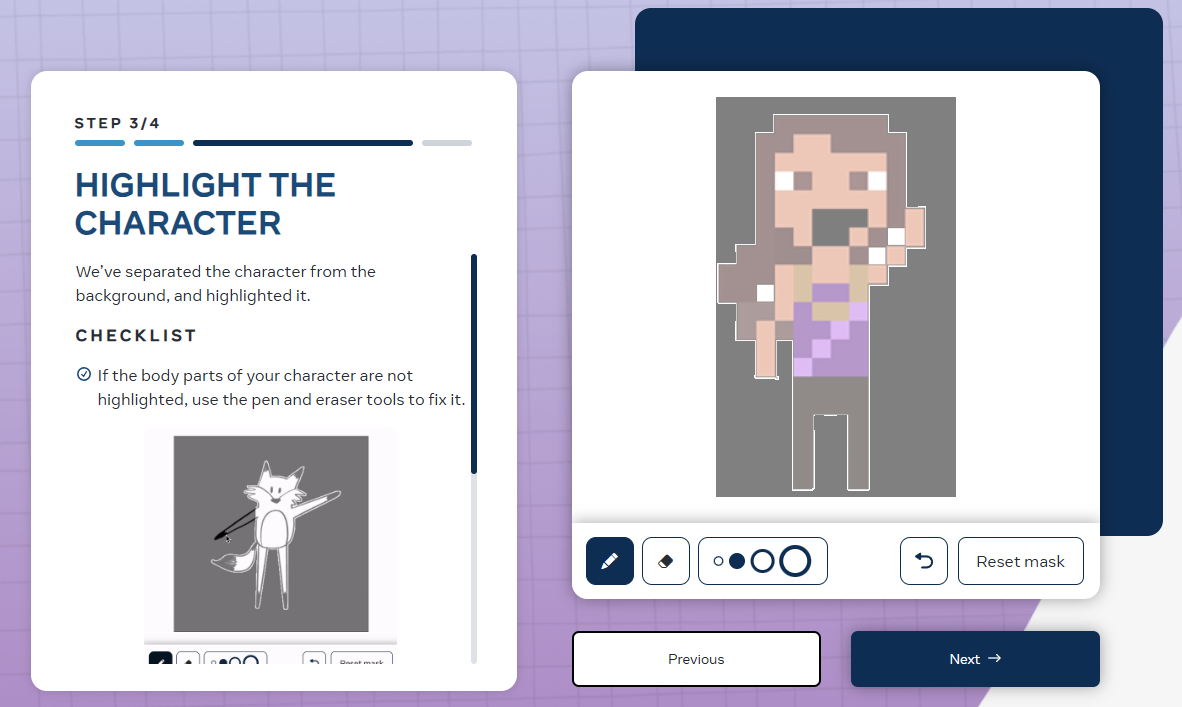
\includegraphics[width=1\linewidth]{figs/sketchLab/tela3.PNG}
        \caption{\small Destacar personagem automático.}
        \label{fig:sketch1c}
    \end{subfigure}
    \begin{subfigure}{0.45\linewidth}
        \centering
        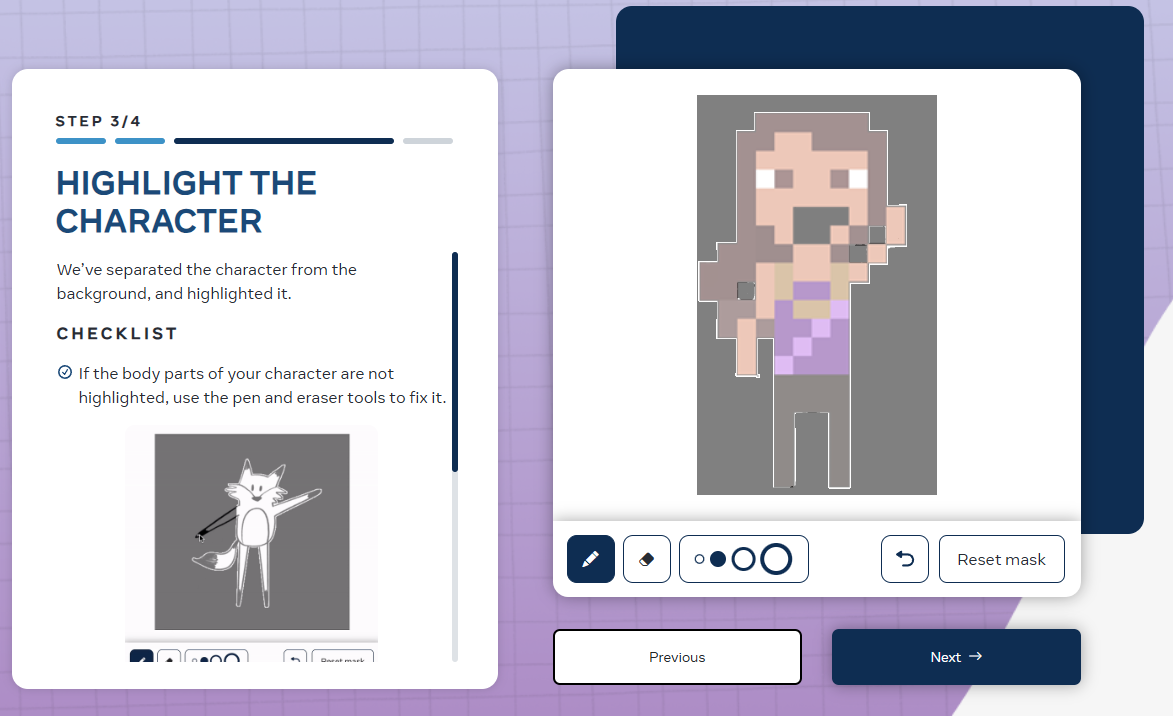
\includegraphics[width=1\linewidth]{figs/sketchLab/tela4.PNG}
        \caption{\small Destacar personagem manual.}
        \label{fig:sketch1d}
    \end{subfigure}
    \begin{subfigure}{0.45\linewidth}
        \centering
        \includegraphics[width=1\linewidth]{figs/sketchLab/tela5.PNG}
        \caption{\small Marcar as articulações do personagem automático.}
        \label{fig:sketch1e}
    \end{subfigure}
    \begin{subfigure}{0.45\linewidth}
        \centering
        \includegraphics[width=1\linewidth]{figs/sketchLab/tela6.PNG}
        \caption{\small Marcar as articulações do personagem manual.}
        \label{fig:sketch1f}
    \end{subfigure}

    \legend{\small Fonte: Elaborada pela autora.}
\end{figure}

\begin{figure}[htbp]
    \centering
    \caption{\small Processo da utilização 2 do Animated Drawnings}
    \label{fig:sketch2}
    \begin{subfigure}{0.6\linewidth}
        \includegraphics[width=1\linewidth]{figs/sketchLab/2tela1.PNG}
        \caption{\small Desenho enviado.}
        \label{fig:sketch2a}
    \end{subfigure}
    \begin{subfigure}{0.45\linewidth}
        \centering
        \includegraphics[width=1\linewidth]{figs/sketchLab/2tela2.PNG}
        \caption{\small Encontrar personagem automático.}
        \label{fig:sketch2b}
    \end{subfigure}
    \begin{subfigure}{0.45\linewidth}
        \centering
        \includegraphics[width=1\linewidth]{figs/sketchLab/2tela3.PNG}
        \caption{\small Encontrar personagem manual.}
        \label{fig:sketch2c}
    \end{subfigure}
    \begin{subfigure}{0.45\linewidth}
        \centering
        \includegraphics[width=1\linewidth]{figs/sketchLab/2tela4.PNG}
        \caption{\small Destacar personagem automático.}
        \label{fig:sketch2d}
    \end{subfigure}
    \begin{subfigure}{0.45\linewidth}
        \centering
        \includegraphics[width=1\linewidth]{figs/sketchLab/2tela5.PNG}
        \caption{\small Destacar personagem manual.}
        \label{fig:sketch2e}
    \end{subfigure}
    \begin{subfigure}{0.45\linewidth}
        \centering
        \includegraphics[width=1\linewidth]{figs/sketchLab/2tela6_2.PNG}
        \caption{\small Marcar as articulações do personagem automático.}
        \label{fig:sketch2f}
    \end{subfigure}
    \begin{subfigure}{0.45\linewidth}
        \centering
        \includegraphics[width=1\linewidth]{figs/sketchLab/2tela7.PNG}
        \caption{\small Marcar as articulações do personagem manual.}
        \label{fig:sketch2g}
    \end{subfigure}

    \legend{\small Fonte: Elaborada pela autora.}
\end{figure}

\begin{figure}[htbp]
    \centering
    \caption{\small Processo da utilização 3 do Animated Drawnings}
    \label{fig:sketch3}
    \begin{subfigure}{0.45\linewidth}
        \includegraphics[width=1\linewidth]{figs/sketchLab/3tela1.PNG}
        \caption{\small Encontrar personagem automático.}
        \label{fig:sketch3a}
    \end{subfigure}
    \begin{subfigure}{0.45\linewidth}
        \centering
        \includegraphics[width=1\linewidth]{figs/sketchLab/3tela2.PNG}
        \caption{\small Encontrar personagem manual.}
        \label{fig:sketch3b}
    \end{subfigure}
    \begin{subfigure}{0.6\linewidth}
        \centering
        \includegraphics[width=1\linewidth]{figs/sketchLab/3tela3.PNG}
        \caption{\small Destacar personagem automático.}
        \label{fig:sketch3c}
    \end{subfigure}
    \begin{subfigure}{0.45\linewidth}
        \centering
        \includegraphics[width=1\linewidth]{figs/sketchLab/3tela4.PNG}
        \caption{\small Marcar as articulações do personagem automático.}
        \label{fig:sketch3d}
    \end{subfigure}
    \begin{subfigure}{0.45\linewidth}
        \centering
        \includegraphics[width=1\linewidth]{figs/sketchLab/3tela6.PNG}
        \caption{\small  Marcar as articulações do personagem manual}
        \label{fig:sketch3e}
    \end{subfigure}
    \legend{\small Fonte: Elaborada pela autora.}
\end{figure}
%   ------------------------------------------------------------------------
\FloatBarrier
\section{God Mode AI}
\label{s.godmodeAIApendice}

\begin{figure}[htbp]
    \centering
    \caption{\small Tela de converter a pixel art para alta resolução}
    \label{fig:godmodAIpixelto3D}
    \includegraphics[width=1\linewidth]{figs/godmodAI/tela pixel art para 3D.PNG}
    \legend{\small Fonte: Elaborada pela autora.}
\end{figure}

\begin{figure}[htbp]
    \centering
    \caption{\small Tela para geração de animação}
    \label{fig:godmodAIGerarAnimacao}
    \begin{subfigure}{1\linewidth}
        \includegraphics[width=1\linewidth]{figs/godmodAI/tela criando animação.PNG}
        \caption{\small Opções de ação e movimento.}
        \label{fig:godmodAIGerarAnimacao1}
    \end{subfigure}
    \legend{\small Fonte: Elaborada pela autora.}
    \begin{subfigure}{1\linewidth}
        \includegraphics[width=1\linewidth]{figs/godmodAI/tela criando animação 2.PNG}
        \caption{\small Reposicionamento.}
        \label{fig:godmodAIGerarAnimacao2}
    \end{subfigure}
    \legend{\small Fonte: Elaborada pela autora.}
\end{figure}

\begin{figure}[htbp]
    \centering
    \caption{\small Tela de converter a animação para pixel art}
    \label{fig:godmodAI3Dtopixel}
    \includegraphics[width=1\linewidth]{figs/godmodAI/video para pixel art.PNG}
    \legend{\small Fonte: Elaborada pela autora.}
\end{figure}

\begin{figure}[htbp]
    \centering
    \caption{\small Interface nova}
    \label{fig:godmodModificado}
    \includegraphics[width=1\linewidth]{figs/godmodAI/site modificado.PNG}
    \legend{\small Fonte: Elaborada pela autora.}
\end{figure}

\begin{figure}[htbp]
    \centering
    \caption{\small Auto reposicionamento no God Mode AI}
    \label{fig:godmodAIrepose}
    \begin{subfigure}{0.35\linewidth}
        \includegraphics[width=1\linewidth]{figs/godmodAI/tela auto repose.PNG}
        \caption{\small Tentativa 1.}
        \label{fig:godmodAIrepose1}
    \end{subfigure}
    \begin{subfigure}{0.35\linewidth}
        \includegraphics[width=1\linewidth]{figs/godmodAI/tela auto repose 2.PNG}
        \caption{\small Tentativa 2.}
        \label{fig:godmodAIrepose2}
    \end{subfigure}
    \begin{subfigure}{0.45\linewidth}
        \includegraphics[width=1\linewidth]{figs/godmodAI/tela auto repose 3.PNG}
        \caption{\small Tentativa 3.}
        \label{fig:godmodAIrepose3}
    \end{subfigure}
        \begin{subfigure}{0.45\linewidth}
        \includegraphics[width=1\linewidth]{figs/godmodAI/tela auto repose 4.PNG}
        \caption{\small Tentativa 4.}
        \label{fig:godmodAIrepose4}
    \end{subfigure}
        \begin{subfigure}{0.45\linewidth}
        \includegraphics[width=1\linewidth]{figs/godmodAI/tela auto repose 5.PNG}
        \caption{\small Tentativa 5.}
        \label{fig:godmodAIrepose5}
    \end{subfigure}
        \begin{subfigure}{0.45\linewidth}
        \includegraphics[width=1\linewidth]{figs/godmodAI/tela auto repose 6.PNG}
        \caption{\small Tentativa 6.}
        \label{fig:godmodAIrepose6}
    \end{subfigure}
    \legend{\small Fonte: Elaborada pela autora, utilizando a ferramenta God Mode AI.}
\end{figure}

\begin{figure}[htbp]
    \centering
    \caption{\small Tela de re-geração parcial}
    \label{fig:godmodAIregen}
    \includegraphics[width=1\linewidth]{figs/godmodAI/regeracao_parcial.PNG}
    \legend{\small Fonte: Elaborada pela autora.}
\end{figure}
%   ------------------------------------------------------------------------
\FloatBarrier
\section{Análise do ChatGPT}
\label{s.chatGPT}

A ferramenta ChatGPT foi selecionada por ser uma interface simples de conversação que usa modelos de IA capazes de gerar imagens e anexar arquivos. O modelo utilizado pelo ChatGPT no período de testes foi o GPT-4o, que não possui como único foco a geração de figuras, também tendo funcionalidades para geração de texto, processamento de linguagem natural, visão computacional (análise visual), entre outros \cite{openaiQuick_2025}. Ele também possui um modelo de geração de imagem nativo, gpt-image-1, capaz de entender textos e figuras, aproveitando seu amplo conhecimento do mundo \cite{openai_2025}. 

Durante a análise, o objetivo principal foi gerar a imagem do personagem Pablo de lado a partir do sprite em diversos ângulos; e o sprite sheet dele andando, usando diferentes imagens como referência. 

\begin{figure}[htbp]
    \centering
    \caption{\small Artefatos usados como referência para geração de imagens no ChatGPT}
    \label{fig:chatGPTArtefatos}
    \begin{subfigure}{0.32\linewidth}
        \includegraphics[width=0.7\linewidth]{figs/sprites/Pablo.PNG}
        \caption{\small Sprite do personagem Pablo em front view}
        \label{fig:chatGPTPablo}
    \end{subfigure}
    \begin{subfigure}{0.32\linewidth}
        \includegraphics[width=1\linewidth]{figs/pixelLab/dia2/fix_init_1.PNG}
        \caption{\small Sprite do personagem Pablo em um ângulo de 90 graus gerado e editado no Pixel Lab}
        \label{fig:chatGPTPablo90}
    \end{subfigure}
    \begin{subfigure}{0.32\linewidth}
        \centering
        \includegraphics[width=1\linewidth]{figs/pixelLab/dia2/fix_teste_3.PNG}
        \caption{\small Sprite do personagem Pablo em um ângulo de 45 graus gerado e editado no Pixel Lab}
        \label{fig:chatGPTPablo45}
    \end{subfigure}
    \begin{subfigure}{0.32\linewidth}
        \includegraphics[width=0.7\linewidth]{figs/geminiPro/melhores/chat2_1.png}
        \caption{\small Imagem 1 do personagem Pablo em side view gerada no Gemini Pro}
        \label{fig:chatGPTPabloGeminiPro1}
    \end{subfigure}
    \begin{subfigure}{0.32\linewidth}
        \includegraphics[width=1\linewidth]{figs/geminiPro/melhores/chat2_2.png}
        \caption{\small Imagem 2 do personagem Pablo em side view gerada no Gemini Pro}
        \label{fig:chatGPTPabloGeminiPro2}
    \end{subfigure}
    \begin{subfigure}{0.32\linewidth}
        \centering
        \includegraphics[width=1\linewidth]{figs/geminiPro/melhores/chat5.PNG}
        \caption{\small Imagem 3 do personagem Pablo em side view gerada no Gemini Pro}
        \label{fig:chatGPTPabloGeminiPro3}
    \end{subfigure}
    \legend{\small Fonte: Elaborada pela autora.}
\end{figure}

%   ------------------------------------------------------------------------
\FloatBarrier
\subsection{Geração do sprite em side view}
\label{s.chatGPT.sideview}

Durante os testes iniciais, foi anexada a Figura \ref{fig:chatGPTPablo}, em sua versão de resolução 16x32, com cada pixel da arte realmente valendo um pixel real. Na primeira tentativa, o prompt utilizado instruía a ferramenta a redesenhar o personagem olhando para o lado direito da tela, o que foi interpretado como o personagem apenas com os olhos virados nessa direção em vez do corpo inteiro. Levando esse fator em conta, ainda na mesma interação, o prompt foi reformulado, especificando melhor qual era a posição desejada. Ambos os resultados gerados mantiveram o estilo de pixel art, a consistência das características e tamanho dos pixels, com cores extremamente similares. Apesar disso, o bracelete que o personagem usava não foi gerado, além de ter sido adicionado um sapato cinza escuro, como pode ser visto na Figura \ref{fig:chatGPTSideViewPixel}. Outro detalhe notado foi que o olho ficou ao máximo à direita, sem nenhum pixel do rosto depois dele, priorizando aparentar ao máximo ser pixel perfect em vez de formar uma imagem mais precisa. A interação completa pode ser consultada na Figura \ref{fig:chatGPT1} no Apêndice \ref{ap.telasIA}.

\begin{figure}[htbp]
    \centering
    \caption{\small Imagem em side view gerada pelo ChatGPT }
    \label{fig:chatGPTSideViewPixel}
    \includegraphics[width=0.3\linewidth]{figs/chatGPT/visao_lateral/res2_pixel.png}
    \legend{\small Fonte: Elaborada pela autora, utilizando a ferramenta ChatGPT.}
\end{figure}

Posteriormente, foi utilizada a mesma imagem de antes, porém em sua versão aumentada, com um prompt textual instruindo a ferramenta a rotacionar o personagem em 90 graus. Além disso, no teste seguinte, também foram anexadas as Figuras \ref{fig:chatGPTPablo90} e \ref{fig:chatGPTPablo45}. Os resultados gerados apresentaram uma melhora na consistência em relação às características, mantendo o bracelete. Porém, foi mais aparente a falta do padrão pixel perfect, além de as imagens formadas apresentarem mais detalhes e tons diferentes, o que resultou em divergências extras com o design original e diferentes formatos de corpo, não tendo uma melhora significativa em comparação com o sprite em side view de referência. O melhor resultado (Figura \ref{fig:chatGPTSideView}) foi gerado antes do anexo dos novos ângulos do personagem para referência, o que indica que as figuras criadas no Pixel Lab diminuíram a performance da geração no ChatGPT. Interação completa demonstrada na Figura \ref{fig:chatGPT2} no Apêndice \ref{ap.telasIA}. 

\begin{figure}[htbp]
    \centering
    \caption{\small Melhor sprite em side view gerado pelo ChatGPT }
    \label{fig:chatGPTSideView}
    \includegraphics[width=0.3\linewidth]{figs/chatGPT/visao_lateral/res1.png}
    \legend{\small Fonte: Elaborada pela autora, utilizando a ferramenta ChatGPT.}
\end{figure}

Na tentativa subsequente, foi iniciado um novo chat para apontar em detalhes o que cada imagem de referência representava, anexando, além da imagem em front view, os melhores sprites gerados em side view (Figuras \ref{fig:chatGPTPabloGeminiPro1} a \ref{fig:chatGPTPabloGeminiPro3} e Figura \ref{fig:chatGPTSideView}). Também foi incluída para contexto a Figura \ref{fig:chatGPTPablo45}, com o intuito de mostrar um meio termo de resultado satisfatório entre a front view e a side view. Os resultados apresentaram um erro de cropping (recorte, em inglês), onde a parte superior e inferior das imagens ficavam fora da tela, sendo cortadas para fora, uma limitação já conhecida da ferramenta \cite{openaiImage_2025}. Isso pode ser visto na Figura \ref{fig:chatGPTCropping}. Foram testados alguns prompts direcionando a IA a editar a imagem e corrigir a falha, porém não foi efetivo, como pode ser consultado na Figura \ref{fig:chatGPT3} no Apêndice \ref{ap.telasIA}.

\begin{figure}[htbp]
    \centering
    \caption{\small Erro no cropping}
    \label{fig:chatGPTCropping}
    \includegraphics[width=0.3\linewidth]{figs/chatGPT/visao_lateral/res4.png}
    \legend{\small Fonte: Elaborada pela autora, utilizando a ferramenta ChatGPT.}
\end{figure}

Apesar do ChatGPT não apresentar melhor performance em comparação com as próximas a serem analisadas, é possível notar sua grande capacidade em manter a consistência e o estilo do personagem, sendo extremamente fácil e acessível de usar. Os erros encontrados não tiveram nenhuma relação com a imagem ser em 2D, e não houve grande dificuldade em gerar uma pixel art, apesar de não ser pixel perfect. O melhor sprite gerado nessa fase (Figura \ref{fig:chatGPTSideView}) vai ser usado como referência durante a análise da Ferramenta Gemini Pro (detalhada na Seção \ref{s.ferramentaB}).


%   ------------------------------------------------------------------------
\FloatBarrier
\subsection{Geração do sprite sheet do personagem andando}
\label{s.chatGPT.spriteSheet}

Para a geração do sprite sheet foram utilizadas duas estratégias: a primeira utilizando apenas o sprite de front view como referência e a segunda utilizando mais imagens para a referência.

Os resultados gerados pelo primeiro método foram insatisfatórios. Apesar de, em geral, haver uma consistência entre a referência e a geração, algumas características eram deixadas de lado, e o estilo de pixel art era ou mais complexo ou mais simples. O principal problema encontrado foi o fato de o sprite sheet apresentar apenas um ou dois sprites substancialmente distintos, com o resto deles sendo basicamente repetidos, como pode ser visto na Figura \ref{fig:chatGPTSpriteSheetFront}.

\begin{figure}[htbp]
    \centering
    \caption{\small Sprite sheet com basicamente a mesma etapa do movimento de andar gerado pelo ChatGPT}
    \label{fig:chatGPTSpriteSheetFront}
    \includegraphics[width=0.6\linewidth]{figs/chatGPT/walking_cycle/front_view/walk cycle 2.png}
    \legend{\small Fonte: Elaborada pela autora, utilizando a ferramenta ChatGPT.}
\end{figure}

Durante a segunda bateria de testes, além de sempre anexar a imagem em front view, no primeiro caso utilizou-se também as imagens geradas pelo Pixel Lab como referência (Figuras \ref{fig:chatGPTPablo90} e \ref{fig:chatGPTPablo45}), enquanto no segundo foi usada como referência a melhor geração do sprite em side view no ChatGPT (Figura \ref{fig:chatGPTSideView}). 

Analisando os resultados, foi notada uma piora na qualidade do produto, com mais deformações nas características, como um terceiro braço ou duas pupilas, e erros em reproduzir a pixel art. Além disso, o sprite sheet ainda é principalmente composto pelo mesmo frame, onde as únicas mudanças não afetam o movimento desejado e apenas alteram a aparência do personagem. Esses detalhes podem ser vistos na Figura \ref{fig:chatGPTSpriteSheetSide}

\begin{figure}[htbp]
    \centering
    \caption{\small Sprite sheet usando a imagem em side view de referência gerado pelo ChatGPT}
    \label{fig:chatGPTSpriteSheetSide}
    \includegraphics[width=0.6\linewidth]{figs/chatGPT/walking_cycle/side_view/walking cycle 2.png}
    \legend{\small Fonte: Elaborada pela autora, utilizando a ferramenta ChatGPT.}
\end{figure}

Em conclusão, o ChatGPT não mostrou-se adequado para tentar criar um sprite sheet, apresentando mais erros em relação à consistência ao tentar criar esse artefato em relação a apenas criar um sprite específico.
%   ------------------------------------------------------------------------
\FloatBarrier
\section{Análise do Pixel Lab}
\label{s.pixelLab}

A plataforma Pixel Lab foi selecionada por seu foco em pixel art, com diversas funcionalidades para o auxílio na criação e refinamento da animação, como:

\begin{itemize}
    \item Ferramenta de rotação;
    \item Animação para animação; e
    \item Edição de imagem.
\end{itemize}


A ferramenta também possui a capacidade de gerar os movimentos de um personagem através do sistema de animação baseado no esqueleto, porém esse recurso não pôde ser testado por ser pago. 

Além disso, existe um editor embutido especificamente para pixel art no ambiente da geração, sendo possível fazer a edição de pixels específicos e tendo outras funcionalidades básicas para a criação e edição de sprites. Esse editor possui uma separação de quadros da animação, podendo receber diretamente o sprite sheet e separar cada uma das imagens em seu respectivo frame, além de também conseguir exportar esse sprite sheet em diversos formatos, com números variados de linhas e colunas (Figura \ref{fig:pixelLabExport} no Apêndice \ref{ap.telasIA}). Apesar de não formar nenhum vídeo diretamente, a ferramenta consegue tocar a animação, considerando todos os quadros ou aqueles pertencentes a uma tag (Figura \ref{fig:pixelLabViewAnimation} no Apêndice \ref{ap.telasIA}). Uma tag pode ser criada clicando com o botão direito do mouse nos números dos frames e selecionando a opção new tag (nova tag, em inglês).

Foi realizado uma série de testes dentro da ferramenta, grande parte deles visando auxiliar na pré-produção de uma animação, (criando imagens de referência), ou no ajuste fino e edições finais do resultado gerado por outra ferramenta.


%%% pablo, pablo lateral de alguma IA, ver tudo que pegou de fora
\begin{figure}[htbp]
    \centering
    \caption{\small Artefatos usados para referência no Pixel Lab}
    \label{fig:pixelLabArtefatos}
    \begin{subfigure}{0.32\linewidth}
        \includegraphics[width=0.7\linewidth]{figs/sprites/Pablo.PNG}
        \caption{\small Sprite do personagem Pablo em front view}
        \label{fig:pixelLabPablo}
    \end{subfigure}
    \begin{subfigure}{0.32\linewidth}
        \includegraphics[width=1\linewidth]{figs/sprites/irma.png}
        \caption{\small Sprite da personagem Luz}
        \label{fig:pixelLabIrma}
    \end{subfigure}
    \begin{subfigure}{1\linewidth}
        \centering
        \includegraphics[width=1\linewidth]{figs/geminiPro/walking_sprite_sheet_grande_pixel.png}
        \caption{\small Sprite sheet gerado pelo Gemini Pro}
        \label{fig:pixelLabSpriteSheetGeminiPro}
    \end{subfigure}
    \begin{subfigure}{1\linewidth}
        \centering
        \includegraphics[width=1\linewidth]{figs/godmodAI/Pixilart/pixilart-sprite.png}
        \caption{\small Sprite sheet gerado pelo God Mode AI}
        \label{fig:pixelLabSpriteSheetGodModeAI}
    \end{subfigure}
    \legend{\small Fonte: Elaborada pela autora.}
\end{figure}

\begin{figure}[htbp]
    \centering
    \caption{\small Artefatos editados no Pixel Lab}
    \label{fig:pixelLabEdicao}
    \begin{subfigure}{0.45\linewidth}
        \centering
        \includegraphics[width=1\linewidth]{figs/geminiPro/fix grande.png}
        \caption{\small Sprite do personagem Pablo em side view gerado pelo Gemini Pro}
        \label{fig:pixelLabPabloGeminiProSide}
    \end{subfigure}
    \begin{subfigure}{0.45\linewidth}
        \centering
        \includegraphics[width=0.8\linewidth]{figs/geminiPro/back_pixel_grande.png}
        \caption{\small Sprite do personagem Pablo de costas gerado pelo Gemini Pro}
        \label{fig:pixelLabPabloGeminiProCostas}
    \end{subfigure}
    \begin{subfigure}{0.45\linewidth}
        \centering
        \includegraphics[width=1\linewidth]{figs/vidu/Pixilart/porta_sprite_sheet_pixel.png}
        \caption{\small Sprite sheet da porta abrindo gerado pelo Vidu}
        \label{fig:pixelLabPortaViduSideView}
    \end{subfigure}
    \begin{subfigure}{0.45\linewidth}
        \centering
        \includegraphics[width=1\linewidth]{figs/sprites/Porta front view.png}
        \caption{\small Sprite da porta em side view fechada}
        \label{fig:pixelLabPortaSideView}
    \end{subfigure}
    \legend{\small Fonte: Elaborada pela autora.}
\end{figure}

%   ------------------------------------------------------------------------
\FloatBarrier
\subsection{Ferramenta de rotação}
\label{s.pixelLab.rotacao}

A ferramenta de rotação possui dois formatos: o componente chamado quick rotate (rotação rápida, em inglês) mostrado na Figura \ref{fig:pixelLabQuickRotateTela} no Apêndice \ref{ap.telasIA}, no qual, após ser selecionado pelo usuário, gera a nova imagem de acordo com o quanto foi arrastado horizontalmente (para definir o ângulo da rotação) e verticalmente (para o ângulo da inclinação) desde o momento do clique do mouse até a sua soltura; e a seção rotate (rotação, em inglês), que abre uma tela com várias configurações para gerar o personagem rotacionado, como pode ser visto na Figura \ref{fig:pixelLabRotateTela} no Apêndice \ref{ap.telasIA}. 

De acordo com a documentação, a ferramenta é melhor em fazer rotações pequenas, de forma que o resultado de uma rotação pode ser usado como a imagem inicial a ser rotacionada. Nesse método, porém, os erros são acumulados a cada rotação. Enquanto isso, há também a possibilidade de apenas fazer a rotação maior para evitar o acúmulo de erros, apesar de ser mais complicado para a IA.

Os testes dessa funcionalidade específica visavam criar a imagem do Pablo em side view, a partir do sprite mostrado na Figura \ref{fig:Pablo}.

Durante as primeiras tentativas, os resultados (Figura \ref{fig:pixelLabRotacao1}) não geraram nenhuma rotação, apenas fazendo deformações no personagem. Porém, foi descoberto em testes posteriores que, para a geração de um bom resultado, o sprite deve estar centralizado no meio da tela, como pode ser visto na Figura \ref{fig:pixelLabRotCompara}.


\begin{figure}[htbp]
    \centering
    \caption{\small Comparação rotação 90 graus no Pixel Lab}
    \label{fig:pixelLabRotCompara}
    \begin{subfigure}{0.45\linewidth}
        \centering
        \includegraphics[width=0.5\linewidth]{figs/pixelLab/dia1/resultado rotacao 2.PNG}
        \caption{\small Resultado a partir do sprite inicialmente no canto esquerdo da tela}
        \label{fig:pixelLabRotComparaCanto}
    \end{subfigure}
    \begin{subfigure}{0.45\linewidth}
        \centering
        \includegraphics[width=0.5\linewidth]{figs/pixelLab/dia2/rot90res1.PNG}
        \caption{\small Resultado a partir do sprite inicialmente no centro da tela}
        \label{fig:pixelLabRotComparaCentro}
    \end{subfigure}

    \legend{\small Fonte: Elaborada pela autora, utilizando a ferramenta Pixel Lab.}
\end{figure}

Dessa forma, os testes prosseguiram posicionando a imagem corretamente, gerando rotações consistentes com o personagem e o estilo, porém com algumas deformações. Analisando os resultados, foi possível perceber que a ferramenta apresenta uma dificuldade na região onde ficaria o nariz, gerando essa parte com mais imperfeições. Além disso, foi notado que existe um processo para conseguir usar somente as cores da imagem de referência:
\begin{itemize}
    \item A imagem é gerada sem restrição nas cores (Figura \ref{fig:pixelLabProcesso1});
    \item A imagem é recriada com tons de cores similares aos da paleta do sprite original, não possuindo restrição no número de tonalidades (Figura \ref{fig:pixelLabProcesso2}); e
    \item O fundo é removido e cada uma das cores é igualada à mais semelhante da paleta original (Figura \ref{fig:pixelLabProcesso3}).
\end{itemize}

\begin{figure}[htbp]
    \centering
    \caption{\small Etapas do processamento da geração de imagem no Pixel Lab}
    \label{fig:pixelLabRotProcesso}
    \begin{subfigure}{0.32\linewidth}
        \centering
        \includegraphics[width=1\linewidth]{figs/pixelLab/dia2/cores_tudo_estranha.PNG}
        \caption{\small Imagem da rotação no início do processamento}
        \label{fig:pixelLabProcesso1}
    \end{subfigure}
    \begin{subfigure}{0.32\linewidth}
        \centering
        \includegraphics[width=1\linewidth]{figs/pixelLab/dia2/perna_antes_de_sumir.PNG}
        \caption{\small Imagem da rotação no meio do processamento, com cores mais parecidas às do sprite original, porém com mais tons}
        \label{fig:pixelLabProcesso2}
    \end{subfigure}
    \begin{subfigure}{0.32\linewidth}
        \centering
        \includegraphics[width=1\linewidth]{figs/pixelLab/dia2/demonstrar_perna_sumindo.PNG}
        \caption{\small Imagem da rotação após o processamento, com cores igualadas ao do sprite original, porém removendo a perna}
        \label{fig:pixelLabProcesso3}
    \end{subfigure}

    \legend{\small Fonte: Elaborada pela autora, utilizando a ferramenta Pixel Lab.}
\end{figure}

Esse processo faz com que nem todas as características do personagem possuam a cor correta, além de muitas vezes causar o desaparecimento da calça por reconhecê-la como parte do fundo, já que as cores são semelhantes. Esses detalhes são mostrados na Figura \ref{fig:pixelLabRotComparaCor}. A demonstração completa dos testes é encontrada nas Figuras \ref{fig:pixelLabRotacao2} a \ref{fig:pixelLabRotacao4}.

\begin{figure}[htbp]
    \centering
    \caption{\small Comparação de cores entre o sprite original e o resultado gerado no Pixel Lab}
    \label{fig:pixelLabRotComparaCor}
    \begin{subfigure}{0.45\linewidth}
        \centering
        \includegraphics[width=1\linewidth]{figs/pixelLab/dia2/sprite_centro.PNG}
        \caption{\small Imagem original com olho castanho escuro e calça completa}
        \label{fig:pixelLabRotComparaCorA}
    \end{subfigure}
    \begin{subfigure}{0.45\linewidth}
        \centering
        \includegraphics[width=1\linewidth]{figs/pixelLab/dia2/rot90res2.PNG}
        \caption{\small Resultado com olho castanho claro e parte da calça faltando}
        \label{fig:pixelLabRotComparaCorB}
    \end{subfigure}

    \legend{\small Fonte: Elaborada pela autora, utilizando a ferramenta Pixel Lab.}
\end{figure}

Na bateria seguinte de testes, foram realizados ajustes finos em algumas das imagens geradas de 45°, com o objetivo de gerar novamente o personagem em 90°, em uma tentativa de contornar o problema dos erros cumulativos. Como a ferramenta possui um editor integrado, é extremamente fácil e eficiente corrigir erros, diferente do que aconteceu em outras ferramentas. As edições feitas podem ser consultadas na Figura \ref{fig:pixelLabAjusteFino1} abaixo e na Figura \ref{fig:pixelLabAjusteFino2} no Apêndice \ref{ap.telasIA}.

\begin{figure}[htbp]
    \centering
    \caption{\small Ajuste fino no resultado da rotação de 45 graus no Pixel Lab}
    \label{fig:pixelLabAjusteFino1}
    \begin{subfigure}{0.45\linewidth}
        \centering
        \includegraphics[width=1\linewidth]{figs/pixelLab/dia2/rot45res4.PNG}
        \caption{\small Antes da edição}
        \label{fig:pixelLabAjusteFino1a}
    \end{subfigure}
    \begin{subfigure}{0.45\linewidth}
        \centering
        \includegraphics[width=1\linewidth]{figs/pixelLab/dia2/fix_teste_4.PNG}
        \caption{\small Após edição}
        \label{fig:pixelLabAjusteFino1b}
    \end{subfigure}

    \legend{\small Fonte: Elaborada pela autora, utilizando a ferramenta Pixel Lab.}
\end{figure}

Após esse ajuste, mais testes foram feitos, porém os resultados gerados (Figuras \ref{fig:pixelLabRotacao6} a \ref{fig:pixelLabRotacao9} no Apêndice \ref{ap.telasIA}) não mostraram nenhuma melhora significativa, aparentando possuir mais deformações e imprecisões do que anteriormente. Isso pode ser melhor notado na Figura \ref{fig:pixelComparaAjuste}.

\begin{figure}[htbp]
    \centering
    \caption{\small Comparação de resultados antes e depois do ajuste fino}
    \label{fig:pixelComparaAjuste}
    \begin{subfigure}{0.45\linewidth}
        \centering
        \includegraphics[width=1\linewidth]{figs/pixelLab/dia2/rot45res4.PNG}
        \caption{\small Resultado gerado a partir da imagem sem o ajuste fino, com uma deformação na região do nariz e boca e erros e pequenos erros na proporção do corpo}
        \label{fig:pixelComparaAjusteAntes}
    \end{subfigure}
    \begin{subfigure}{0.45\linewidth}
        \centering
        \includegraphics[width=1\linewidth]{figs/pixelLab/dia2/rot45fix3res2.PNG}
        \caption{\small Resultado gerado a partir da imagem com o ajuste fino, onde apenas a cabeça do sprite gerado aparenta estar rotacionada e com um deformação no olho}
        \label{fig:pixelComparaAjusteDepois}
    \end{subfigure}

    \legend{\small Fonte: Elaborada pela autora, utilizando a ferramenta Pixel Lab.}
\end{figure}

Considerando a falha na abordagem anterior, uma nova estratégia foi montada considerando uma das opções de customização que a ferramenta rotate oferece: init image (imagem de inicialização, em inglês). Essa funcionalidade permite ao usuário indicar uma imagem para guiar a IA em como deve ficar o resultado final, tendo uma variável associada chamada init image strength (força da imagem de inicialização, em inglês) para indicar o quanto essa inicialização deve ser utilizada. 

Na primeira instância, o melhor resultado gerado do personagem em side view na ferramenta é usado como imagem de inicialização, como pode ser visto na Figura \ref{fig:pixelLabRotInit} no Apêndice \ref{ap.telasIA}.

Os resultados gerados (Figura \ref{fig:pixelLabRotacao10} no Apêndice \ref{ap.telasIA}) apresentaram uma melhor performance comparada aos sprites gerados sem nenhuma imagem de inicialização, porém demonstraram erros na região da calça, o que também pode ser visto na imagem de inicialização, apesar de com menos intensidade. Devido a esse fator, foi feita uma edição na init image, que pode ser vista na Figura \ref{fig:pixelLabAjusteFino3}.

\begin{figure}[htbp]
    \centering
    \caption{\small Edição no resultado da rotação de 90 graus no Pixel Lab}
    \label{fig:pixelLabAjusteFino3}
    \begin{subfigure}{0.45\linewidth}
        \centering
        \includegraphics[width=1\linewidth]{figs/pixelLab/dia2/init.PNG}
        \caption{\small Antes da edição}
        \label{fig:pixelLabAjusteFino3a}
    \end{subfigure}
    \begin{subfigure}{0.45\linewidth}
        \centering
        \includegraphics[width=1\linewidth]{figs/pixelLab/dia2/fix_init_1.PNG}
        \caption{\small Após edição}
        \label{fig:pixelLabAjusteFino3b}
    \end{subfigure}

    \legend{\small Fonte: Elaborada pela autora, utilizando a ferramenta Pixel Lab.}
\end{figure}

Analisando as imagens geradas (Figura \ref{fig:pixelLabRotacao11} no Apêndice \ref{ap.telasIA}) ainda não foi encontrado nenhum resultado satisfatório, com todos os sprites gerados sem as pernas.

Reavaliando todos os resultados, apesar da ferramenta quase ter gerado resultados satisfatórios, nenhum dos sprites alcança os padrões de qualidade para sua aplicação no jogo. Porém, a Figura \ref{fig:pixelLabAjusteFino2c} no Apêndice \ref{ap.telasIA} e a Figura  \ref{fig:pixelLabAjusteFino3b} foram usadas como referência para fornecer um contexto maior do personagem nas ferramentas ChatGPT (detalhada na Seção \ref{s.chatGPT}) e GeminiPro (detalhada na Seção \ref{s.ferramentaB}).

A análise da funcionalidade de rotação indica que, embora a ferramenta não elimine a necessidade de intervenção manual, ela otimiza o processo de criação. Os resultados, embora exijam edições e ajustes finos para atingir a qualidade desejada, fornecem uma base com alta consistência e fidelidade que auxilia na produção dos sprites do personagem.


%   ------------------------------------------------------------------------
\FloatBarrier
\subsection{Ferramenta de animação para animação}
\label{s.pixelLab.animacao}

A ferramenta de animation to animation (animação para animação, em inglês) utiliza o sprite de uma pessoa e uma animação qualquer como referências para animar o movimento desse personagem. A funcionalidade pode gerar até 15 frames e também usa uma descrição do personagem a ser animado e da ação a ser feita, com opções de customização do contorno e shading (sombreamento, em inglês) que o resultado final deve ter. A  funcionalidade de limitação de cores considera a paleta do primeiro frame da animação de base, e não do sprite de referência. Existem também duas variáveis que influenciam a geração: AI freedom (liberdade da IA, em inglês), que determina o quanto a IA deve imitar a animação de referência; e guidance weight (peso da orientação, em inglês), que indica o quanto a descrição influencia no resultado.

O objetivo da primeira bateria de testes dessa funcionalidade foi gerar uma animação do personagem Pablo andando, utilizando como base o sprite sheet gerado pela ferramenta God Mode AI (Figura \ref{fig:pixelLabSpriteSheetGodModeAI}). Antes de ser usada como referência, a imagem gerada pela ferramenta Gemini Pro (detalhada na Seção \ref{s.ferramentaB}) do personagem Pablo em side view (Figura \ref{fig:pixelLabPabloGeminiProSide}) passou por ajustes finos, como pode ser visto na Figura \ref{fig:pixelLabAniSideViewSprite1}. É importante notar que este sprite representa uma versão intermediária do resultado final da edição. Análises posteriores levaram a um refinamento adicional, cujo processo é detalhado na Seção \ref{s.pixelLab.edicao}, resultando na versão final utilizada no jogo.

\begin{figure}[htbp]
    \centering
    \caption{\small Sprite do personagem em side view após ajuste fino}
    \label{fig:pixelLabAniSideViewSprite1}
    \includegraphics[width=0.4\linewidth]{figs/pixelLab/dia3/fixGrande.PNG}
    \legend{\small Fonte: Elaborada pela autora.}
\end{figure}

Durante o teste inicial, a imagem corrigida e a animação citada anteriormente são colocadas como referência, enquanto é utilizado um prompt simples que descreve as roupas usadas pelo personagem, como pode ser verificado na Figura \ref{fig:pixelLabAniTela}.


\begin{figure}[htbp]
    \centering
    \caption{\small Tela da geração de animação no Pixel Lab}
    \label{fig:pixelLabAniTela}
    \includegraphics[width=1\linewidth]{figs/pixelLab/dia3/tela_animacao.PNG}
    \legend{\small Fonte: Elaborada pela autora.}
\end{figure}

O resultado gerado\footnote{\url{https://drive.google.com/file/d/1TYecwF1D5EqbKaJIOJle_iZbkVOuWsux/view?usp=sharing}} foi insatisfatório, apresentando uma aparência diferente do personagem de referência, além de não possuir o mesmo estilo de pixel art, como pode ser visto na Figura \ref{fig:pixelLabAniResRuim}.

\begin{figure}[htbp]
    \centering
    \caption{\small Quadro da animação gerada no Pixel Lab}
    \label{fig:pixelLabAniResRuim}
    \includegraphics[width=0.4\linewidth]{figs/pixelLab/dia3/print1.PNG}
    \legend{\small Fonte: Elaborada pela autora.}
\end{figure}

Levando em conta esse erro, em testes posteriores foi adicionada a descrição da aparência do personagem no prompt como pode ser verificado na Figura \ref{fig:pixelLabAniPrompt}. Durante cada uma das interações, algumas palavras do prompt e as configurações de sombreamento são mudadas, visando obter um resultado mais consistente com o sprite de referência. As tentativas completas podem ser consultadas nas Figuras \ref{fig:pixelLabAnimacao1} a \ref{fig:pixelLabAnimacao6} do Apêndice \ref{ap.telasIA}. 

\begin{figure}[htbp]
    \centering
    \caption{\small Prompt com a descrição da aparência}
    \label{fig:pixelLabAniPrompt}
    \includegraphics[width=0.7\linewidth]{figs/pixelLab/dia3/prompt.PNG}
    \legend{\small Fonte: Elaborada pela autora.}
\end{figure}

A geração de uma animação possui o mesmo processo da geração de imagem, o que faz sentido considerando que um vídeo é formado por várias figuras (quadros). 

Durante um dos testes, ocorreu algo inesperado: nenhuma animação foi gerada. Investigando mais a fundo, foi descoberto que, na última etapa do processamento, onde o fundo deveria ser removido, o sprite inteiro foi deletado. Esse erro não se repetiu em mais nenhum outro teste. Abaixo se encontram as Figuras \ref{fig:pixelLabAniPromptFalha} e \ref{fig:pixelLabAniTelaFalha} mostrando o prompt usado e o resultado gerado na interação falha.


\begin{figure}[htbp]
    \centering
    \caption{\small Prompt que gerou a falha no Pixel Lab}
    \label{fig:pixelLabAniPromptFalha}
    \includegraphics[width=0.53\linewidth]{figs/pixelLab/dia3/tela_3.PNG}
    \legend{\small Fonte: Elaborada pela autora.}
\end{figure}

\begin{figure}[htbp]
    \centering
    \caption{\small Quadros vazios após a geração no Pixel Lab}
    \label{fig:pixelLabAniTelaFalha}
    \includegraphics[width=0.7\linewidth]{figs/pixelLab/dia3/falha3.PNG}
    \legend{\small Fonte: Elaborada pela autora.}
\end{figure}

Analisando os resultados, nenhum deles manteve o formato da silhueta original, os tons de cores ficaram levemente distintos do personagem a ser animado e possuíam falhas de pixels que tornavam as características do rosto menos reconhecíveis. Foi possível notar que o tamanho e a forma do sprite da animação de referência influenciaram as imagens geradas, o que pode ser observado mais atentamente na Figura \ref{fig:pixelLabAnimaCompara}. Investigando mais a fundo, isso acontece por causa do funcionamento da funcionalidade animação para animação, que cria o esqueleto da animação de referência, e usa a movimentação que o esqueleto apresentou para criar uma nova animação. O esqueleto da animação de base mantém o formato e o tamanho da mesma, e o resultado final é gerado por cima desse esqueleto, utilizando as características deste.

\begin{figure}[htbp]
    \centering
    \caption{\small Comparação do sprite original com os frames da animação de base e da gerada no Pixel Lab}
    \label{fig:pixelLabAnimaCompara}

    \begin{subfigure}{0.32\linewidth}
        \includegraphics[width=0.9\linewidth]{figs/pixelLab/dia3/print0.PNG}
        \caption{\small Frames da animação de referência}
        \label{fig:pixelLabAnimaComparaAni}
    \end{subfigure}
    \begin{subfigure}{0.32\linewidth}
        \includegraphics[width=1\linewidth]{figs/pixelLab/dia3/print4.PNG}
        \caption{\small Frame da animação gerada }
        \label{fig:pixelLabAnimaComparaGera}
    \end{subfigure}
    \begin{subfigure}{0.32\linewidth}
        \includegraphics[width=0.9\linewidth]{figs/pixelLab/dia3/fixGrande.PNG}
        \caption{\small Sprite original em side view }
        \label{fig:pixelLabAnimaComparaSprite}
    \end{subfigure}
    \legend{\small Fonte: Elaborada pela autora, utilizando a ferramenta Pixel Lab.}
\end{figure}


A análise mostra que usar a ferramenta com uma animação que não é consistente com o sprite em tamanho e formato não gera resultados satisfatórios que possam ser aplicados em um jogo. Considerando esse fator, posteriormente foi realizada uma segunda bateria de testes, utilizando para a geração da nova animação o sprite sheet do vídeo do personagem Pablo andando gerado pela ferramenta Gemini Pro (Figura \ref{fig:pixelLabSpriteSheetGeminiPro}), que possui características extremamente próximas ao sprite original, porém apresenta pequenos erros. Além disso, como imagem de referência será usada a versão final do ajuste fino do sprite do personagem Pablo em side view gerado pelo Gemini Pro (Figura \ref{fig:pixelLabAniSideViewSprite2}).

\begin{figure}[htbp]
    \centering
    \caption{\small Quadro da animação gerada no Pixel Lab}
    \label{fig:pixelLabAniSideViewSprite2}
    \includegraphics[width=0.4\linewidth]{figs/pixelLab/dia3/fix_oficial_fundo_igual.PNG}
    \legend{\small Fonte: Elaborada pela autora.}
\end{figure}

Os resultados\footnote{\url{https://drive.google.com/drive/folders/1xmE-wpvT9xLguyX2izbWv2Xn0glh84IZ?usp=sharing}} gerados obtiveram uma alta consistência, porém a qualidade deles foi menor do que a da animação de referência, com tons de cores diferentes do sprite original e erros nos pixels, porém possuindo o formato mais preciso da mão, como pode ser visto na Figura \ref{fig:pixelLabAnimaComparaGemini}. A interação completa pode ser consultada nas Figuras \ref{fig:pixelLabAnimacao7} e \ref{fig:pixelLabAnimacao8} do Apêndice \ref{ap.telasIA}. 

\begin{figure}[htbp]
    \centering
    \caption{\small Comparação do sprite de referência com os frames da animação de base e da gerada no Pixel Lab}
    \label{fig:pixelLabAnimaComparaGemini}

    \begin{subfigure}{0.32\linewidth}
        \includegraphics[width=1\linewidth]{figs/pixelLab/dia4/print0.PNG}
        \caption{\small Frame da animação de referência, com cores mais precisas e dedão na mão visível}
        \label{fig:pixelLabAnimaComparaGeminiAni}
    \end{subfigure}
    \begin{subfigure}{0.32\linewidth}
        \includegraphics[width=1\linewidth]{figs/pixelLab/dia3/fix_oficial_fundo_igual.PNG}
        \caption{\small Sprite de referência em side view, sem dedão visível na mão}
        \label{fig:pixelLabAnimaComparaGeminiSprite}
    \end{subfigure}
    \begin{subfigure}{0.32\linewidth}
        \includegraphics[width=1\linewidth]{figs/pixelLab/dia4/print1.PNG}
        \caption{\small Frame da animação gerada, com cores menos precisas e sem dedão na mão}
        \label{fig:pixelLabAnimaComparaGeminiGera}
    \end{subfigure}
    \legend{\small Fonte: Elaborada pela autora, utilizando a ferramenta Pixel Lab.}
\end{figure}

Nos testes posteriores, além de se utilizar a opção de limitar as cores da animação gerada de acordo com a paleta do primeiro frame, o mesmo foi editado para ter as cores exatas do sprite original. O objetivo era testar a capacidade da ferramenta na geração da animação, sem buscar apenas produzir uma animação melhor pela edição manual. Como a animação mostrada parcialmente na Figura \ref{fig:pixelLabAnimaComparaGeminiGera}, apesar de ter tons de cores diferentes, possui um formato mais preciso, ela também foi utilizada como referência após a do sprite original como primeiro quadro. 

Os resultados\footnote{\url{https://drive.google.com/drive/folders/1YHiklOXkW1FhYC_fBS00c21wt8fMNiIq?usp=drive_link}} obtiveram uma queda na qualidade, com as cores sendo utilizadas de maneira imprecisa e possuindo ainda mais erros nos pixels, como pode ser visto na Figura \ref{fig:pixelLabAnimaComparaGemini2}. Interações completas podem ser consultadas nas Figuras \ref{fig:pixelLabAnimacao9} a \ref{fig:pixelLabAnimacao11} no Apêndice \ref{ap.telasIA}. Investigando mais a fundo, é descoberto que esse declínio provavelmente foi causado pelo fato de que o sprite original não possui tons suficientes para trazer um efeito de profundidade na região das pernas e dos braços, fazendo a IA aplicar cores totalmente diferentes em regiões que precisam ter essa diferença.

\begin{figure}[htbp]
    \centering
    \caption{\small Comparação do sprite de referência com os frames das animações geradas no Pixel Lab}
    \label{fig:pixelLabAnimaComparaGemini2}

    \begin{subfigure}{0.32\linewidth}
        \includegraphics[width=1\linewidth]{figs/pixelLab/dia4/print1.PNG}
        \caption{\small Frame da animação gerada sem limitar as cores para apenas as mesmas do sprite de referência}
        \label{fig:pixelLabAnimaComparaGeminiAni2}
    \end{subfigure}
    \begin{subfigure}{0.32\linewidth}
        \includegraphics[width=1\linewidth]{figs/pixelLab/dia3/fix_oficial_fundo_igual.PNG}
        \caption{\small Sprite de referência em side view}
        \label{fig:pixelLabAnimaComparaGeminiSprite2}
    \end{subfigure}
    \begin{subfigure}{0.32\linewidth}
        \includegraphics[width=1\linewidth]{figs/pixelLab/dia4/print6.PNG}
        \caption{\small Frame da animação gerada limitando as cores para apenas as mesmas do sprite de referência}
        \label{fig:pixelLabAnimaComparaGeminiGera2}
    \end{subfigure}
    \legend{\small Fonte: Elaborada pela autora, utilizando a ferramenta Pixel Lab.}
\end{figure}

Para explorar os limites da ferramenta, foi conduzido um último teste. O objetivo era verificar se essa funcionalidade também poderia ser utilizada para gerar uma animação de rotação completa, uma tarefa normalmente designada à ferramenta de rotação. 

Para isso, foi criada manualmente uma animação de pseudo-rotação utilizando os sprites já existentes do personagem Pablo (visão frontal, lateral, de costas e lateral espelhada), cada um ocupando um quadro para simular um giro de 360 graus. Esta animação serviu como referência de movimento. Como sprite de referência, foi utilizada a personagem Luz, que possui um corpo com proporções e tamanho significativamente diferentes. Naquele momento, ainda não havia sido compreendido totalmente que a animação gerada seguia o formato da animação de referência e não do sprite.

O resultado\footnote{\url{https://drive.google.com/file/d/1NEfmTRU46067ueFgWvvhpd1MQBiyhP1H/view?usp=sharing}} gerado foi completamente insatisfatório, produzindo uma animação completamente deformada que tentava aplicar as proporções maiores do personagem Pablo ao corpo menor da personagem Luz. Este experimento serviu como confirmação definitiva da teoria levantada nos testes anteriores: a ferramenta prioriza a estrutura geométrica e as proporções do esqueleto da animação de referência, em vez de seguir o formato do sprite de referência. A inconsistência dimensional entre os dois inputs leva inevitavelmente a um resultado de baixa precisão, como pode ser visto na Figura \ref{fig:pixelLabAnimaComparaRodarSprite}.

\begin{figure}[htbp]
    \centering
    \caption{\small Comparação do sprite original com os frames da animação gerada no Pixel Lab}
    \label{fig:pixelLabAnimaComparaRodar}

    \begin{subfigure}{0.32\linewidth}
        \includegraphics[width=1\linewidth]{figs/pixelLab/dia4/irma.PNG}
        \caption{\small Sprite original}
        \label{fig:pixelLabAnimaComparaRodarSprite}
    \end{subfigure}
    \begin{subfigure}{0.32\linewidth}
        \includegraphics[width=1\linewidth]{figs/pixelLab/dia4/printA.PNG}
        \caption{\small Frame 1 da animação gerada }
        \label{fig:pixelLabAnimaComparaRodarFrame1}
    \end{subfigure}
    \begin{subfigure}{0.32\linewidth}
        \includegraphics[width=1\linewidth]{figs/pixelLab/dia4/printB.PNG}
        \caption{\small Frame 2 da animação gerada  }
        \label{fig:pixelLabAnimaComparaRodarFrame2}
    \end{subfigure}
    \legend{\small Fonte: Elaborada pela autora, utilizando a ferramenta Pixel Lab.}
\end{figure}

A análise revela que a ferramenta é capaz de gerar animações consistentes se a animação de referência é parecida com o sprite, porém o resultado formado ainda exige ajustes finos, possuindo falhas de pixels e tons de cores não idênticos aos desejados, o que faz com que sua performance na geração não alcance a mesma qualidade comparada às ferramentas descritas nas próximas seções. Apesar disso, assim como a funcionalidade de rotação, a criação de animação baseada em outra animação apresenta grande potencial de otimização do processo em cenário com uma animação base de alta qualidade ou com diversos personagens de tamanho e forma parecidos.


%   ------------------------------------------------------------------------
\FloatBarrier
\subsection{Uso no pós-processamento}
\label{s.pixelLab.edicao}


Um dos principais usos do PixelLab.AI neste projeto foi como ferramenta de pós-processamento, aplicando ajustes finos manuais nos resultados gerados por outras ferramentas de forma que o resultado final já podia ser diretamente aplicado no jogo. A forma de exportação, o editor embutido e o ambiente em pixel art foram funcionalidades que trouxeram eficiência para essa etapa de correções, que é justamente o que falta na maioria das outras ferramentas.

Nessa seção, abordaremos as edições feitas que geraram o resultado final.

Como comentado em seções anteriores, o sprite do personagem Pablo em side view gerado pela ferramenta Gemini Pro (Figura \ref{fig:pixelLabPabloGeminiProSide}) passou por uma correção, onde os tons de cores e o tamanho foram ajustados, comparando o sprite lado a lado com a imagem do mesmo personagem de frente como pode ser visto nas Figuras \ref{fig:pixelLabFixSideViewComparaAntes} e \ref{fig:pixelLabFixSideViewComparaDepois}. Esse processo é extremamente importante, pois durante o jogo, o sprite de um personagem deve ser realmente consistente com os outros sprites daquele personagem, uma vez que haverá transições entre cada uma dessas figuras. Se a consistência não se mantém, em vez de apenas demonstrar um movimento ou mudança de posição, é causado um estranhamento no jogador. Posteriormente, uma nova edição foi realizada para ajustar detalhes como a falta de cabelo na nuca e o formato da orelha. Esse processo é demonstrado na Figura \ref{fig:pixelLabFinalSideView}.

\begin{figure}[htbp]
    \centering
    \caption{\small Comparação do sprite original e sprite gerado pelo Gemini Pro antes da edição}
    \label{fig:pixelLabFixSideViewComparaAntes}
    \includegraphics[width=0.4\linewidth]{figs/pixelLab/dia3/comparacao.PNG}
    \legend{\small Fonte: Elaborada pela autora.}
\end{figure}
    
\begin{figure}[htbp]
    \centering
    \caption{\small Comparação do sprite original e sprite gerado pelo Gemini Pro depois da edição}
    \label{fig:pixelLabFixSideViewComparaDepois}
    \includegraphics[width=0.4\linewidth]{figs/pixelLab/dia3/fix.PNG}
    \legend{\small Fonte: Elaborada pela autora, utilizando a ferramenta Pixel Lab.}
\end{figure}

\begin{figure}[htbp]
    \centering
    \caption{\small Processo de edição no Pixel Lab do sprite em side view gerado pelo Gemini Pro}
    \label{fig:pixelLabFinalSideView}
    \begin{subfigure}{0.32\linewidth}
        \centering
        \includegraphics[width=1\linewidth]{figs/pixelLab/dia3/semFix.PNG}
        \caption{\small Antes da edição no Pixel Lab}
        \label{fig:pixelLabFinalSideView1}
    \end{subfigure}
    \begin{subfigure}{0.32\linewidth}
        \centering
        \includegraphics[width=1\linewidth]{figs/pixelLab/dia3/fixGrande.PNG}
        \caption{\small Após a primeira edição no Pixel Lab}
        \label{fig:pixelLabFinalSideView2}
    \end{subfigure}
    \begin{subfigure}{0.32\linewidth}
        \centering
        \includegraphics[width=1\linewidth]{figs/pixelLab/dia3/fix_oficial_fundo_igual.PNG}
        \caption{\small Resultado final}
        \label{fig:pixelLabFinalSideView3}
    \end{subfigure}

    \legend{\small Fonte: Elaborada pela autora, utilizando a ferramenta Pixel Lab.}
\end{figure}

Também foram realizados ajustes finos na, anteriormente apresentada, Figura \ref{fig:pixelLabPabloGeminiProCostas}, que mostra o sprite do personagem Pablo de costas gerado pelo Gemini Pro (detalhado na Seção \ref{s.ferramentaB}). O processo foi parecido com o do personagem em side view, usando a visão de frente para corrigir as cores e o tamanho da imagem. Além disso, pixels do que antes era o fundo branco foram apagados, mantendo a imagem com um fundo transparente. Esse processo pode ser verificado na Figura \ref{fig:pixelLabFinalBackView}.

\begin{figure}[htbp]
    \centering
    \caption{\small Processo de edição no Pixel Lab do sprite em back view gerado pelo Gemini Pro}
    \label{fig:pixelLabFinalBackView}
    \begin{subfigure}{0.45\linewidth}
        \centering
        \includegraphics[width=1\linewidth]{figs/pixelLab/dia3/back_sem_fix.PNG}
        \caption{\small Antes da edição no Pixel Lab}
        \label{fig:pixelLabFinalBackView1}
    \end{subfigure}
    \begin{subfigure}{0.45\linewidth}
        \centering
        \includegraphics[width=1\linewidth]{figs/pixelLab/dia3/back_fix.PNG}
        \caption{\small Resultado final}
        \label{fig:pixelLabFinalBackView2}
    \end{subfigure}


    \legend{\small Fonte: Elaborada pela autora, utilizando a ferramenta Pixel Lab.}
\end{figure}

Os ajustes finos feitos no sprite sheet da porta abrindo em side view (Figura \ref{fig:pixelLabPortaViduSideView}) gerada pelo Vidu (detalhado na Seção \ref{s.vidu}) foram parcialmente parecidos com os anteriores, usando o sprite da porta fechada (Figura \ref{fig:pixelLabPortaSideView} para corrigir a altura, além de retirar qualquer pixel branco. Além disso, a moldura da porta (presente no sprite) foi fixada na mesma posição em todos os quadros, pois a moldura deve permanecer igual sem se mover mesmo quando a porta é aberta. Após isso, para cada um dos quadros, foi apagada a maçaneta ainda ligada à moldura, pintada novamente aquela parte da porta e desenhada uma nova maçaneta no canto correto. Após 12 quadros (dos 31 totais), foi observada que a porta praticamente não ficava mais aberta, com a maior parte dos outros frames igual ou muito similares. Dessa forma, os frames restantes foram apagados para não ocorrer perda de tempo em mudanças insignificantes.

A parte mais complexa do processo foi fazer novamente a maçaneta, pois era necessário entender o formato correto que ela ficaria dependendo do ângulo e como representar essa forma através dos tons de cores. Apesar disso, foi uma tarefa muito mais simples e rápida do que fazer a porta inteira do zero múltiplas vezes com cada frame tendo apenas pequenas modificações. O resultado desse processo final de edição pode ser verificado na Figura \ref{fig:pixelLabFinalPortaSideView}.

\begin{figure}[htbp]
    \centering
    \caption{\small Processo de edição no Pixel Lab do sprite sheet da porta gerado pelo Vidu}
    \label{fig:pixelLabFinalPortaSideView}
    \begin{subfigure}{0.45\linewidth}
        \centering
        \includegraphics[width=1\linewidth]{figs/vidu/Pixilart/porta_sprite_sheet_pixel.png}
        \caption{\small Antes da edição no Pixel Lab}
        \label{fig:pixelLabFinalPortaSideView1}
    \end{subfigure}
    \begin{subfigure}{0.45\linewidth}
        \centering
        \includegraphics[width=1\linewidth]{figs/pixelLab/final/side_door_pixel_vidu.png}
        \caption{\small Resultado final}
        \label{fig:pixelLabFinalPortaSideView2}
    \end{subfigure}


    \legend{\small Fonte: Elaborada pela autora, utilizando a ferramenta Pixel Lab.}
\end{figure}
%   ------------------------------------------------------------------------
\FloatBarrier
\section{Análise do OpenArt.AI}
\label{s.openArt}

A ferramenta OpenArt AI foi selecionada para análise pela sua capacidade de edição de imagens por chat e geração de vídeos, agregando múltiplos modelos de IA para isso. A plataforma possui outros módulos interessantes (Figura \ref{fig:openArtModulos} no Apêndice \ref{ap.telasIA}) além dos que foram testados, como o módulo de personagem, que não pôde ser investigado pela limitação de créditos. Como base, todo usuário ao se cadastrar recebe 40 créditos grátis, sendo possível aumentar esse valor seguindo os canais da ferramenta em diferentes redes sociais.

O objetivo durante os testes foi gerar uma animação ou sprite do personagem Pablo sentado em front view, utilizando o sprite dele em pé como referência. O objeto onde o personagem se senta não deveria aparecer na imagem ou vídeo formado, pois a ideia era usar a mesma animação de sentar para qualquer objeto.

Primeiro, foi averiguado o módulo de vídeo, que fornecia diversas funcionalidades diferentes para a geração da animação (Figura \ref{fig:openArtModuloVideo} no Apêndice \ref{ap.telasIA}), porém só foi possível testar apenas uma delas. As funções que pareciam mais adequadas com o objetivo foram: Imagem para Vídeo e Elementos para Vídeo. Explorando melhor a interface e instruções das duas, foi escolhida a ferramenta de Elementos para Vídeo, porque a outra não permitia o uso de um prompt textual, criando um vídeo apenas com a imagem anexada sem nenhuma instrução.

A ferramenta permitia anexar até 7 elementos para o vídeo, todavia apenas o sprite do personagem foi anexado para não aparecer nenhum outro objeto em cena. Havia dois modelos de IA disponíveis para uso, Vidu Q1 e Kling 1.6 (Figura \ref{fig:openArtModelosVideo} no Apêndice \ref{ap.telasIA}). Analisando as opções, o Vidu Q1 foi considerado o mais adequado, pois o outro era mais especializado para fotorrealismo. Foi utilizado um prompt descrevendo como deveria ser a animação de sentar em detalhes, que pode ser consultado no Quadro \ref{quad:openArtPrompt}. A tela para geração do vídeo pode ser consultada na Figura \ref{fig:openArtVideo} no Apêndice \ref{ap.telasIA}.

\begin{figure}[htbp]
    \centering
    \captionof{quadro}{Prompt textual detalhado para geração de vídeo no OpenArt.AI.}
    \label{quad:openArtPrompt}
    \fbox{                                  % Este comando cria uma caixa ao redor do texto
        \begin{minipage}{0.9\textwidth}     % Define a largura da caixa de texto
            \vspace{1ex}                    % Adiciona um pequeno espaço no topo
            \textit{Create a 2D pixel art animation using the provided character. The animation should show the character moving from his current standing pose into a sitting position. Crucially, he is sitting on an object, like a chair or a couch. The animation frames should depict him bending his knees, lowering his hips, and leaning back slightly until he settles into a natural, relaxed sitting posture, suspended in mid-air. His final pose should look like he is being comfortably supported by something. Maintain the exact pixel art style, colors, and design of the character throughout the entire animation.}
            
            \vspace{2ex}                    % Adiciona um espaço entre o original e a tradução
            
            \noindent\textbf{Tradução livre:} Crie uma animação 2D em pixel art usando o personagem fornecido. A animação deve mostrar o personagem se movendo de sua pose atual em pé para uma posição sentada. Crucialmente, ele está sentado em um objeto, como uma cadeira ou um sofá. Os quadros da animação devem retratá-lo dobrando os joelhos, baixando os quadris e inclinando-se ligeiramente para trás até que ele se acomode em uma postura sentada natural e relaxada, suspenso no ar. Sua pose final deve parecer que ele está sendo confortavelmente apoiado por algo. Mantenha o estilo de pixel art, cores e design exatos do personagem durante toda a animação.
            \vspace{1ex}                    % Adiciona um pequeno espaço na base
        \end{minipage}
    }
    
    \legend{\small Fonte: Elaborada pela autora.}
\end{figure}

O resultado \footnote{\url{https://drive.google.com/file/d/1tCKdj0FJEHVoq5y0V6qRCAkA7e2ZNrcz/view?usp=sharing}} gerado foi insatisfatório, fazendo uma animação 3D onde o personagem é rotacionado e mexe a cabeça para cima antes de sentar em side view. O movimento de sentar também não é muito preciso, onde é parada a movimentação no meio por alguns momentos, para depois o personagem se agachar completamente, alguns segundos depois movendo as pernas para frente e para baixo do nível inicial do chão. Apesar disso, a ferramenta foi capaz de manter as características físicas consistentes e permitiu a exportação em gif. A Figura \ref{fig:openArtVideoFrames} apresenta frames da animação gerada.

\begin{figure}[htbp]
    \centering
    \caption{\small Frames do vídeo gerado no OpenArt.AI}
    \label{fig:openArtVideoFrames}
    \begin{subfigure}{0.45\linewidth}
    \centering
        \includegraphics[width=0.65\linewidth]{figs/OpenArtAI/frame1.jpg}
        \caption{\small Primeiro frame}
        \label{fig:openArtVideoFrames1}
    \end{subfigure}
    \begin{subfigure}{0.45\linewidth}
    \centering
        \includegraphics[width=0.65\linewidth]{figs/OpenArtAI/frame2.jpg}
        \caption{\small Último frame}
        \label{fig:openArtVideoFrames2}
    \end{subfigure}
    \legend{\small Fonte: Elaborada pela autora, utilizando a ferramenta OpenArt.AI.}
\end{figure}

Devido à geração do vídeo não ser bem-sucedida, os próximos testes focaram na geração de apenas o sprite do personagem sentado. Explorando o módulo de imagem, havia diversas funcionalidades (Figura \ref{fig:openArtModuloImagem} no Apêndice \ref{ap.telasIA}), porém apenas duas delas se mostraram acessíveis e adequadas para a análise: criar imagem e chat para editar. Foi escolhida a funcionalidade de chat para editar, pois em tese a consistência do personagem seria garantida.

A ferramenta de chat para editar apresentava várias opções de modelo de IA (Figura \ref{fig:openArtModelosImagem} no Apêndice \ref{ap.telasIA}) com diferentes níveis de geração. Uma interação com cada modelo foi realizada, visando editar o personagem em pé para a posição de sentado. Foi utilizado o mesmo prompt para os testes com diferentes modelos.

O modelo SeeEdit parece estar escrito de forma incorreta na plataforma. Durante pesquisas, não foi possível encontrar um modelo com esse nome específico, apenas outro extremamente similar chamado SeedEdit 3.0 da BytePlus. O logo da empresa BytePlus coincidiu com o logo ao lado do SeeEdit no OpenArtAI, o que concretiza a hipótese do erro de digitação. O SeedEdit é um modelo de edição de imagens através de instruções de texto, se destacando em modificar áreas-chave com precisão, mantendo outras informações detalhadas com alta consistência \cite{modelark-byteplus_2025}. O resultado gerado foi satisfatório, sem mudar nenhuma região desnecessária do personagem, mantendo a característica e proporção da perna e mantendo o ambiente em 2D, porém perdendo a característica do estilo de pixel art na área específica modificada. Essa incongruência não chamou tanta atenção pois ainda se manteve o estilo simples, inclinando o que reto parecia formar uma pixel art, e as duas curvas realizadas não ficaram destoantes. É possível verificar isso na Figura \ref{fig:openArtSeedEdit}.

\begin{figure}[htbp]
    \centering
    \caption{\small Imagem gerada pelo modelo SeedEdit no OpenArtAI}
    \label{fig:openArtSeedEdit}
    \includegraphics[width=0.2\linewidth]{figs/OpenArtAI/seeEdit.png}
    \legend{\small Fonte: Elaborada pela autora,utilizando a ferramenta OpenArt.AI.}
\end{figure}

O Flux Kontext é uma família de modelos que utilizam o método flow matching (correspondência de fluxo, em inglês) para geração e edição de imagens. Diferente do modelo Flux, ele é capaz de entender imagens existentes e modificá-las de acordo com instruções de texto simples \cite{blackforestlabs_2025}. O resultado gerado foi quase satisfatório, mantendo o personagem e o estilo consistente, porém gerando a cadeira, adicionando um sapato cinza escuro e com uma perna mais grossa que a outra. A Figura \ref{fig:openArtFluxKontext} apresenta esse resultado.

\begin{figure}[htbp]
    \centering
    \caption{\small Imagem gerada pelo modelo Flux Kontext Pro no OpenArtAI}
    \label{fig:openArtFluxKontext}
    \includegraphics[width=0.2\linewidth]{figs/OpenArtAI/fluxKontextPro.png}
    \legend{\small Fonte: Elaborada pela autora,utilizando a ferramenta OpenArt.AI.}
\end{figure}

O Gemini é um modelo de IA capaz de entender, operar e combinar diversos tipos de dados, como texto e imagem \cite{sundarpichai_2023}. Porém, na plataforma OpenArt.AI não foi encontrada nenhuma informação específica sobre a versão do modelo. O resultado gerado não foi satisfatório, pois, apesar de manter a consistência, foi desenhada uma cadeira em outro estilo e ângulo, o personagem não foi bem encaixado no assento e os joelhos ficaram dobrados para cima. Imagem mostrada na Figura \ref{fig:openArtGemini}.

\begin{figure}[htbp]
    \centering
    \caption{\small Imagem gerada pelo modelo Gemini no OpenArtAI}
    \label{fig:openArtGemini}
    \includegraphics[width=0.2\linewidth]{figs/OpenArtAI/gemini.png}
    \legend{\small Fonte: Elaborada pela autora,utilizando a ferramenta OpenArt.AI.}
\end{figure}

Testando o mesmo prompt diretamente no Gemini Pro, os resultados não foram melhores e continuou havendo problemas de precisão, como pode ser visto na Figura \ref{fig:openArtComparaGemini}.

\begin{figure}[htbp]
    \centering
    \caption{\small Imagens geradas pelo modelo Gemini}
    \label{fig:openArtComparaGemini}
    \begin{subfigure}{0.32\linewidth}
    \centering
        \includegraphics[width=1\linewidth]{figs/OpenArtAI/gemini.png}
        \caption{\small Resultado gerado dentro do OpenArtAI}
        \label{fig:openArtComparaGemini1}
    \end{subfigure}
    \begin{subfigure}{0.32\linewidth}
    \centering
        \includegraphics[width=0.8\linewidth]{figs/geminiPro/compararDalle3_res.PNG}
        \caption{\small Resultado 1 gerado dentro do Gemini Pro}
        \label{fig:openArtComparaGemini2}
    \end{subfigure}
    \begin{subfigure}{0.32\linewidth}
    \centering
        \includegraphics[width=1\linewidth]{figs/geminiPro/compararDalle3_res2.PNG}
        \caption{\small Resultado 2 gerado dentro do Gemini Pro}
        \label{fig:openArtComparaGemini3}
    \end{subfigure}
    \legend{\small Fonte: Elaborada pela autora, utilizando a ferramenta OpenArt.AI e Gemini Pro.}
\end{figure}

Diferente do ChatGPT, que é a aplicação de chatbot oficial da OpenAI, o GPT é o modelo utilizado, como já foi explicado na Seção \ref{s.chatGPT}. O resultado foi insatisfatório, alterando levemente os tons de cores e o tamanho do personagem, além de mudar o ângulo em 45 graus. Apesar disso, a imagem manteve o estilo de pixel art e as características em geral do personagem, não mostrando a cadeira. A Figura \ref{fig:openArtComparaGPT} compara o personagem original com o sprite gerado.

\begin{figure}[htbp]
    \centering
    \caption{\small Comparação do sprite original e do sprite gerado pelo modelo GPT no OpenArt.AI}
    \label{fig:openArtComparaGPT}
    \begin{subfigure}{0.45\linewidth}
    \centering
        \includegraphics[width=0.5\linewidth]{figs/sprites/Pablo.PNG}
        \caption{\small Sprite original}
        \label{fig:openArtComparaGPTOriginal}
    \end{subfigure}
    \begin{subfigure}{0.45\linewidth}
    \centering
        \includegraphics[width=0.5\linewidth]{figs/OpenArtAI/gpt.png}
        \caption{\small Resultado gerado pelo GPT no OpenArtAI}
        \label{fig:openArtComparaGPTGerado}
    \end{subfigure}
    \legend{\small Fonte: Elaborada pela autora, utilizando a ferramenta OpenArt.AI e Gemini Pro.}
\end{figure}


Todas as interações podem ser consultadas nas Figuras \ref{fig:openArtModeloSeedEdit} a \ref{fig:openArtModeloGPT} no Apêndice \ref{ap.telasIA}.

Apesar da animação gerada não ter sido satisfatória, o OpenArt.AI demonstrou grande potencial na edição de imagem, servindo como uma excelente ferramenta para a iteração de edições. Nenhum modelo individual foi capaz de gerar um resultado sem erros, porém deve-se notar que a análise foi limitada a uma única iteração por modelo devido à restrição de créditos. Funcionalidades de edição via chat são iterativas, projetadas para que o usuário aponte as falhas de uma geração e a IA as corrija em tentativas subsequentes. A impossibilidade de realizar este ciclo de refinamento pode ter impactado o desempenho final de cada modelo.

Apesar da animação gerada não ter sido satisfatória, o OpenArt.AI demonstrou grande potencial na edição de imagem, servindo como uma excelente ferramenta para a iteração e ideação de poses. Nenhum modelo individual foi capaz de gerar um resultado final sem erros, contudo, é fundamental ressaltar que a análise foi limitada a uma única iteração por modelo devido à restrição de créditos. Funcionalidades de edição via chat são inerentemente iterativas, projetadas para que o usuário aponte as falhas de uma geração e a IA as corrija em tentativas subsequentes. A impossibilidade de realizar este ciclo de refinamento pode ter impactado o desempenho final de cada modelo.

%tentei iteração com gemini, e ficou melhor do que o primeiro resultado da iteração nova, mas foi meio esquisito como se comportou
%   ------------------------------------------------------------------------
\FloatBarrier
\section{Vidu}
\label{s.viduApendice}

\begin{figure}[htbp]
    \centering
    \caption{\small Processo da utilização do Vidu em junho/2025}
    \label{fig:vidu1}
    \begin{subfigure}{0.75\linewidth}
        \includegraphics[width=1\linewidth]{figs/vidu/tela.PNG}
        \caption{\small Prompt}
        \label{fig:vidu1a}
    \end{subfigure}
    \begin{subfigure}{0.2\linewidth}
        \includegraphics[width=1\linewidth]{figs/vidu/frame1.jpg}
        \caption{\small Frame do vídeo gerado}
        \label{fig:vidu1b}
    \end{subfigure}
    \begin{subfigure}{0.75\linewidth}
        \centering
        \includegraphics[width=0.4\linewidth]{figs/vidu/tela2_real.PNG}
        \caption{\small Prompt adicionando a palavra 2D}
        \label{fig:vidu1c}
    \end{subfigure}
    \begin{subfigure}{0.2\linewidth}
        \includegraphics[width=1\linewidth]{figs/vidu/frame2.jpg}
        \caption{\small Frame do vídeo gerado}
        \label{fig:vidu1d}
    \end{subfigure}
    \begin{subfigure}{0.75\linewidth}
        \centering
        \includegraphics[width=1\linewidth]{figs/vidu/tela2.PNG}
        \caption{\small Prompt adicionando a palavra pixel art e não usando o imagem 1 como sujeito}
        \label{fig:vidu1e}
    \end{subfigure}
    \begin{subfigure}{0.2\linewidth}
        \includegraphics[width=1\linewidth]{figs/vidu/frame3.jpg}
        \caption{\small Frame do vídeo gerado}
        \label{fig:vidu1f}
    \end{subfigure}
    \legend{\small Fonte: Elaborada pela autora, utilizando a ferramenta Vidu.}
\end{figure}

\begin{figure}[htbp]
    \centering
    \caption{\small Processo da utilização 1 do Vidu em julho/2025}
    \label{fig:vidu2}
    \begin{subfigure}{0.4\linewidth}
        \includegraphics[width=1\linewidth]{figs/vidu/tela3.PNG}
        \caption{\small Prompt}
        \label{fig:vidu2a}
    \end{subfigure}
    \begin{subfigure}{0.2\linewidth}
        \includegraphics[width=1\linewidth]{figs/vidu/frame4.jpg}
        \caption{\small Frame do vídeo 1 gerado}
        \label{fig:vidu2b}
    \end{subfigure}
    \begin{subfigure}{0.2
    \linewidth}
        \includegraphics[width=1\linewidth]{figs/vidu/frame4.2.jpg}
        \caption{\small Frame do vídeo 2 gerado}
        \label{fig:vidu2c}
    \end{subfigure}

    \legend{\small Fonte: Elaborada pela autora, utilizando a ferramenta Vidu.}
\end{figure}

\begin{figure}[htbp]
    \centering
    \caption{\small Processo da utilização 2 do Vidu em julho/2025}
    \label{fig:vidu3}
    \begin{subfigure}{0.4\linewidth}
        \includegraphics[width=1\linewidth]{figs/vidu/tela4.PNG}
        \caption{\small Prompt adicionando a palavra 2D e mudança de proporção}
        \label{fig:vidu3a}
    \end{subfigure}
    \begin{subfigure}{0.4\linewidth}
        \includegraphics[width=1\linewidth]{figs/vidu/frame5_2D.jpg}
        \caption{\small Frame 1 do vídeo gerado, aparentando ser 2D}
        \label{fig:vidu3b}
    \end{subfigure}
    \begin{subfigure}{0.4\linewidth}
        \includegraphics[width=1\linewidth]{figs/vidu/frame5_3D.jpg}
        \caption{\small Frame 2 do vídeo gerado, em 3D}
        \label{fig:vidu3c}
    \end{subfigure}

    \legend{\small Fonte: Elaborada pela autora, utilizando a ferramenta Vidu.}
\end{figure}

\begin{figure}[htbp]
    \centering
    \caption{\small Processo da utilização 3 do Vidu em julho/2025}
    \label{fig:vidu4}
    \begin{subfigure}{0.6\linewidth}
        \includegraphics[width=1\linewidth]{figs/vidu/tela5.PNG}
        \caption{\small Prompt utilizando a tag da imagem como sujeito}
        \label{fig:vidu4a}
    \end{subfigure}
    \begin{subfigure}{0.35\linewidth}
        \includegraphics[width=1\linewidth]{figs/vidu/frame6.jpg}
        \caption{\small Frame do vídeo gerado}
        \label{fig:vidu4b}
    \end{subfigure}
    \legend{\small Fonte: Elaborada pela autora, utilizando a ferramenta Vidu.}
\end{figure}

\begin{figure}[htbp]
    \centering
    \caption{\small Processo da utilização 4 do Vidu em julho/2025}
    \label{fig:vidu5}
    \begin{subfigure}{0.4\linewidth}
        \includegraphics[width=1\linewidth]{figs/vidu/tela5_2.PNG}
        \caption{\small Prompt especificando o fundo sem nada}
        \label{fig:vidu5a}
    \end{subfigure}
    \begin{subfigure}{0.4\linewidth}
        \includegraphics[width=1\linewidth]{figs/vidu/frame6_2.jpg}
        \caption{\small Frame do vídeo gerado}
        \label{fig:vidu5b}
    \end{subfigure}
    \legend{\small Fonte: Elaborada pela autora, utilizando a ferramenta Vidu.}
\end{figure}



\begin{figure}[htbp]
    \centering
    \caption{\small Tela da criação da referência da beliche no Vidu}
    \label{fig:viduReferenciaCama}
    \begin{subfigure}{0.4\linewidth}
        \includegraphics[width=1\linewidth]{figs/vidu/tela_referencia_beliche.PNG}
        \caption{\small Parte 1 da descrição}
        \label{fig:viduReferenciaCama1}
    \end{subfigure}
    \begin{subfigure}{0.45\linewidth}
        \includegraphics[width=1\linewidth]{figs/vidu/tela_referencia_beliche2.PNG}
        \caption{\small Parte 2 da descrição}
        \label{fig:viduReferenciaCama2}
    \end{subfigure}
    \legend{\small Fonte: Elaborada pela autora.}
\end{figure}


\begin{figure}[htbp]
    \centering
    \caption{\small Tela da criação da referência da porta marrom no Vidu}
    \label{fig:viduReferenciaPortaA}
    \begin{subfigure}{0.4\linewidth}
        \includegraphics[width=1\linewidth]{figs/vidu/tela_referencia_porta.PNG}
        \caption{\small Parte 1 da descrição}
        \label{fig:viduReferenciaPortaA1}
    \end{subfigure}
    \begin{subfigure}{0.4\linewidth}
        \includegraphics[width=1\linewidth]{figs/vidu/tela_referencia_porta_2.PNG}
        \caption{\small Parte 2 da descrição}
        \label{fig:viduReferenciaPortaA2}
    \end{subfigure}
    \legend{\small Fonte: Elaborada pela autora.}
\end{figure}

\begin{figure}[htbp]
    \centering
    \caption{\small Tela da criação da referência da porta cinza no Vidu}
    \label{fig:viduReferenciaPortaC}
    \includegraphics[width=0.4\linewidth]{figs/vidu/tela_referencia_porta_tutorial.PNG}
    \legend{\small Fonte: Elaborada pela autora.}
\end{figure}

\begin{figure}[htbp]
    \centering
    \caption{\small Tela da criação da referência do quarto do Pablo no Vidu}
    \label{fig:viduReferenciaQuarto}
    \begin{subfigure}{0.4\linewidth}
        \includegraphics[width=1\linewidth]{figs/vidu/tela_referencia_quarto.PNG}
        \caption{\small Parte 1 da descrição}
        \label{fig:viduReferenciaQuarto1}
    \end{subfigure}
    \begin{subfigure}{0.4\linewidth}
        \includegraphics[width=1\linewidth]{figs/vidu/tela_referencia_quarto2.PNG}
        \caption{\small Parte 2 da descrição}
        \label{fig:viduReferenciaQuarto2}
    \end{subfigure}
    \legend{\small Fonte: Elaborada pela autora.}
\end{figure}

\begin{figure}[htbp]
    \centering
    \caption{\small Tela da criação da referência da cena do tutorial no Vidu}
    \label{fig:viduReferenciaTutorial}
    \begin{subfigure}{0.4\linewidth}
        \includegraphics[width=1\linewidth]{figs/vidu/tela_referencia_tutorial.PNG}
        \caption{\small Parte 1 da descrição}
        \label{fig:viduReferenciaTutorial1}
    \end{subfigure}
    \begin{subfigure}{0.4\linewidth}
        \includegraphics[width=1\linewidth]{figs/vidu/tela_referencia_tutorial_2.PNG}
        \caption{\small Parte 2 da descrição}
        \label{fig:viduReferenciaTutorial2}
    \end{subfigure}
    \legend{\small Fonte: Elaborada pela autora.}
\end{figure}


\begin{figure}[htbp]
    \centering
    \caption{\small Processo da utilização 1 do Vidu em agosto/2025}
    \label{fig:vidu6}
    \begin{subfigure}{0.35\linewidth}
        \includegraphics[width=1\linewidth]{figs/vidu/tela6.PNG}
        \caption{\small Prompt}
        \label{fig:vidu6a}
    \end{subfigure}
    \begin{subfigure}{0.55\linewidth}
        \includegraphics[width=1\linewidth]{figs/vidu/frame6_real.jpg}
        \caption{\small Frame do vídeo gerado}
        \label{fig:vidu6b}
    \end{subfigure}
    \legend{\small Fonte: Elaborada pela autora, utilizando a ferramenta Vidu.}
\end{figure}

\begin{figure}[htbp]
    \centering
    \caption{\small Processo da utilização 2 do Vidu em agosto/2025}
    \label{fig:vidu7}
    \begin{subfigure}{0.35\linewidth}
        \includegraphics[width=1\linewidth]{figs/vidu/tela7.PNG}
        \caption{\small Prompt}
        \label{fig:vidu7a}
    \end{subfigure}
    \begin{subfigure}{0.55\linewidth}
        \includegraphics[width=1\linewidth]{figs/vidu/frame7.jpg}
        \caption{\small Frame do vídeo gerado}
        \label{fig:vidu7b}
    \end{subfigure}
    \legend{\small Fonte: Elaborada pela autora, utilizando a ferramenta Vidu.}
\end{figure}

\begin{figure}[htbp]
    \centering
    \caption{\small Processo da utilização 3 do Vidu em agosto/2025}
    \label{fig:vidu8}
    \begin{subfigure}{0.35\linewidth}
        \includegraphics[width=1\linewidth]{figs/vidu/tela8.PNG}
        \caption{\small Prompt}
        \label{fig:vidu8a}
    \end{subfigure}
    \begin{subfigure}{0.55\linewidth}
        \includegraphics[width=1\linewidth]{figs/vidu/frame8.jpg}
        \caption{\small Frame do vídeo gerado}
        \label{fig:vidu8b}
    \end{subfigure}
    \legend{\small Fonte: Elaborada pela autora, utilizando a ferramenta Vidu.}
\end{figure}

\begin{figure}[htbp]
    \centering
    \caption{\small Processo da utilização 4 do Vidu em agosto/2025}
    \label{fig:vidu9}
    \begin{subfigure}{0.35\linewidth}
        \includegraphics[width=1\linewidth]{figs/vidu/tela9.PNG}
        \caption{\small Prompt}
        \label{fig:vidu9a}
    \end{subfigure}
    \begin{subfigure}{0.55\linewidth}
        \includegraphics[width=1\linewidth]{figs/vidu/frame9.jpg}
        \caption{\small Frame do vídeo gerado}
        \label{fig:vidu9b}
    \end{subfigure}
    \legend{\small Fonte: Elaborada pela autora, utilizando a ferramenta Vidu.}
\end{figure}

\begin{figure}[htbp]
    \centering
    \caption{\small Edição da referência do personagem no Vidu}
    \label{fig:viduReferenciaPabloEditado}
    \includegraphics[width=0.4\linewidth]{figs/vidu/tela_referencia_2_editado2.PNG}
    \legend{\small Fonte: Elaborada pela autora.}
\end{figure}

\begin{figure}[htbp]
    \centering
    \caption{\small Processo da utilização 5 do Vidu em agosto/2025}
    \label{fig:vidu10}
    \begin{subfigure}{0.35\linewidth}
        \includegraphics[width=1\linewidth]{figs/vidu/tela10.PNG}
        \caption{\small Prompt}
        \label{fig:vidu10a}
    \end{subfigure}
    \begin{subfigure}{0.55\linewidth}
        \includegraphics[width=1\linewidth]{figs/vidu/frame10.jpg}
        \caption{\small Frame do vídeo gerado}
        \label{fig:vidu10b}
    \end{subfigure}
    \legend{\small Fonte: Elaborada pela autora, utilizando a ferramenta Vidu.}
\end{figure}

\begin{figure}[htbp]
    \centering
    \caption{\small Processo da utilização 6 do Vidu em agosto/2025}
    \label{fig:vidu11}
    \begin{subfigure}{0.35\linewidth}
        \includegraphics[width=1\linewidth]{figs/vidu/tela11.PNG}
        \caption{\small Prompt}
        \label{fig:vidu11a}
    \end{subfigure}
    \begin{subfigure}{0.55\linewidth}
        \includegraphics[width=1\linewidth]{figs/vidu/frame11.PNG}
        \caption{\small Frame do vídeo gerado}
        \label{fig:vidu11b}
    \end{subfigure}
    \legend{\small Fonte: Elaborada pela autora, utilizando a ferramenta Vidu.}
\end{figure}

\begin{figure}[htbp]
    \centering
    \caption{\small Processo da utilização 7 do Vidu em agosto/2025}
    \label{fig:vidu12}
    \begin{subfigure}{0.35\linewidth}
        \includegraphics[width=1\linewidth]{figs/vidu/tela12.PNG}
        \caption{\small Prompt}
        \label{fig:vidu12a}
    \end{subfigure}
    \begin{subfigure}{0.55\linewidth}
        \includegraphics[width=1\linewidth]{figs/vidu/frame12.jpg}
        \caption{\small Frame do vídeo gerado}
        \label{fig:vidu12b}
    \end{subfigure}
    \legend{\small Fonte: Elaborada pela autora, utilizando a ferramenta Vidu.}
\end{figure}

\begin{figure}[htbp]
    \centering
    \caption{\small Processo da utilização 8 do Vidu em agosto/2025}
    \label{fig:vidu13}
    \begin{subfigure}{0.42\linewidth}
        \includegraphics[width=1\linewidth]{figs/vidu/tela13.PNG}
        \caption{\small Prompt}
        \label{fig:vidu13a}
    \end{subfigure}
    \begin{subfigure}{0.52\linewidth}
        \includegraphics[width=1\linewidth]{figs/vidu/tela13_resto.PNG}
        \caption{\small Continuação do prompt}
        \label{fig:vidu13b}
    \end{subfigure}
    \begin{subfigure}{0.55\linewidth}
        \includegraphics[width=1\linewidth]{figs/vidu/frame13.jpg}
        \caption{\small Frame do vídeo gerado}
        \label{fig:vidu13c}
    \end{subfigure}
    \legend{\small Fonte: Elaborada pela autora, utilizando a ferramenta Vidu.}
\end{figure}


\begin{figure}[htbp]
    \centering
    \caption{\small Processo de geração da animação de pulo pela funcionalidade Referência para vídeo no Vidu}
    \label{fig:viduPulo1}
    \begin{subfigure}{0.55\linewidth}
        \includegraphics[width=1\linewidth]{figs/vidu/PULO_tela01.PNG}
        \caption{\small Prompt}
        \label{fig:viduPulo1a}
    \end{subfigure}
    \begin{subfigure}{0.45\linewidth}
        \includegraphics[width=1\linewidth]{figs/vidu/framePulo1.jpg}
        \caption{\small Frame do vídeo 1 gerado}
        \label{fig:viduPulo1b}
    \end{subfigure}
    \begin{subfigure}{0.45\linewidth}
        \includegraphics[width=1\linewidth]{figs/vidu/framePulo1_2.jpg}
        \caption{\small Frame do vídeo gerado}
        \label{fig:viduPulo1c}
    \end{subfigure}
    \legend{\small Fonte: Elaborada pela autora, utilizando a ferramenta Vidu.}
\end{figure}

\begin{figure}[htbp]
    \centering
    \caption{\small Processo de geração da animação 1 da porta no Vidu }
    \label{fig:viduPorta1}
    \begin{subfigure}{0.42\linewidth}
        \includegraphics[width=1\linewidth]{figs/vidu/porta_tela1.PNG}
        \caption{\small Prompt}
        \label{fig:viduPorta1a}
    \end{subfigure}
    \begin{subfigure}{0.42\linewidth}
        \includegraphics[width=1\linewidth]{figs/vidu/porta_tela2.PNG}
        \caption{\small Prompt}
        \label{fig:viduPorta1b}
    \end{subfigure}
    \begin{subfigure}{0.32\linewidth}
        \includegraphics[width=1\linewidth]{figs/vidu/framePorta1.jpg}
        \caption{\small Continuação do prompt}
        \label{fig:viduPorta1c}
    \end{subfigure}
    \legend{\small Fonte: Elaborada pela autora, utilizando a ferramenta Vidu.}
\end{figure}

\begin{figure}[htbp]
    \centering
    \caption{\small Processo de geração da animação 2 da porta no Vidu }
    \label{fig:viduPorta2}
    \begin{subfigure}{0.42\linewidth}
        \includegraphics[width=1\linewidth]{figs/vidu/porta_tela1.PNG}
        \caption{\small Prompt}
        \label{fig:viduPorta2a}
    \end{subfigure}
    \begin{subfigure}{0.42\linewidth}
        \includegraphics[width=1\linewidth]{figs/vidu/porta_tela3.PNG}
        \caption{\small Prompt}
        \label{fig:viduPorta2b}
    \end{subfigure}
    \begin{subfigure}{0.32\linewidth}
        \includegraphics[width=1\linewidth]{figs/vidu/framePorta2.jpg}
        \caption{\small Continuação do prompt}
        \label{fig:viduPorta2c}
    \end{subfigure}
    \legend{\small Fonte: Elaborada pela autora, utilizando a ferramenta Vidu.}
\end{figure}

\begin{figure}[htbp]
    \centering
    \caption{\small Animação da porta cinza pela funcionalidade Imagem para vídeo no Vidu }
    \label{fig:vidu14}
    \begin{subfigure}{0.42\linewidth}
        \includegraphics[width=1\linewidth]{figs/vidu/tela14.PNG}
        \caption{\small Prompt}
        \label{fig:vidu14a}
    \end{subfigure}
    \begin{subfigure}{0.42\linewidth}
        \includegraphics[width=1\linewidth]{figs/vidu/frame14.jpg}
        \caption{\small Quadro do vídeo gerado}
        \label{fig:vidu14b}
    \end{subfigure}
    \legend{\small Fonte: Elaborada pela autora, utilizando a ferramenta Vidu.}
\end{figure}

\begin{figure}[htbp]
    \centering
    \caption{\small Animação da porta marrom pela funcionalidade Imagem para vídeo no Vidu }
    \label{fig:vidu15}
    \begin{subfigure}{0.35\linewidth}
        \includegraphics[width=1\linewidth]{figs/vidu/tela15.PNG}
        \caption{\small Prompt}
        \label{fig:vidu15a}
    \end{subfigure}
    \begin{subfigure}{0.35\linewidth}
        \includegraphics[width=1\linewidth]{figs/vidu/framePortaSanfona.jpg}
        \caption{\small Quadro do vídeo gerado}
        \label{fig:vidu15b}
    \end{subfigure}
    \begin{subfigure}{0.35\linewidth}
        \includegraphics[width=1\linewidth]{figs/vidu/tela16.PNG}
        \caption{\small Prompt adicionando a direção para qual a porta deve abrir}
        \label{fig:vidu15c}
    \end{subfigure}
    \begin{subfigure}{0.35\linewidth}
        \includegraphics[width=1\linewidth]{figs/vidu/framePortaAberta.jpg}
        \caption{\small Quadro do vídeo gerado}
        \label{fig:vidu15d}
    \end{subfigure}
    \legend{\small Fonte: Elaborada pela autora, utilizando a ferramenta Vidu.}
\end{figure}

\begin{figure}[htbp]
    \centering
    \caption{\small Processo de geração da animação de pulo pela funcionalidade Imagem para vídeo no Vidu}
    \label{fig:viduPulo2}
    \begin{subfigure}{0.45\linewidth}
        \includegraphics[width=1\linewidth]{figs/vidu/PULO_tela02.PNG}
        \caption{\small Prompt}
        \label{fig:viduPulo2a}
    \end{subfigure}
    \begin{subfigure}{0.45\linewidth}
        \includegraphics[width=1\linewidth]{figs/vidu/framePuloDobra.jpg}
        \caption{\small Frame do vídeo gerado}
        \label{fig:viduPulo2b}
    \end{subfigure}
    \legend{\small Fonte: Elaborada pela autora, utilizando a ferramenta Vidu.}
\end{figure}

\begin{figure}[htbp]
    \centering
    \caption{\small Processo de geração da animação definitiva da porta em side view no Vidu}
    \label{fig:viduFinal}
    \begin{subfigure}{0.45\linewidth}
        \includegraphics[width=1\linewidth]{figs/vidu/porta_tela4.PNG}
        \caption{\small Prompt}
        \label{fig:viduFinalPrompt}
    \end{subfigure}
    \begin{subfigure}{0.45\linewidth}
        \includegraphics[width=1\linewidth]{figs/vidu/frameFinal2.jpg}
        \caption{\small Frame do vídeo gerado}
        \label{fig:viduFinalQuadro}
    \end{subfigure}
    \legend{\small Fonte: Elaborada pela autora, utilizando a ferramenta Vidu.}
\end{figure}


\FloatBarrier
\section{Análise da Ferramenta Gemini Pro}
\label{s.ferramentaB}


\FloatBarrier
\section{Quadro comparativo e discussão geral}
\label{s.quadroComparativo}

\FloatBarrier
\section{Desenvolvimento de um fluxo de trabalho para animação com IA}
\label{s.pipeline}
\chapter{Conclusão}
\label{c.conclusao}

Os arquivos estão sendo concatenados. Podemos continuar a nossa escrita em outro arquivo .tex desde que ele seja importado no projeto principal, que é sempre o utilizado para efetuar a compilação.
\appendix
\chapter{Capturas de Tela da Análise de Ferramentas de IA}
\label{ap.telasIA}


%   ------------------------------------------------------------------------
\FloatBarrier
\section{Visão geral da análise comparativa}
\label{s.visaoAnalise}

Como já foi mencionado, a aplicação de IA para a criação de animações 2D não foi muito explorada, tendo um potencial muito grande a ser descoberto. Atualmente, a maioria das ferramentas generativas de vídeo é voltada para ambientes tridimensionais e realistas. Diante desse cenário, esta análise busca investigar a capacidade e o resultado das tecnologias atuais quando aplicadas ao contexto da animação 2D para um jogo.

Durante a análise preliminar, uma das ferramentas foi imediatamente descartada do estudo por não ser capaz de gerar resultados. A ferramenta AI Sprite Sheet Maker, encontrada na plataforma segmind, foi inicialmente selecionada por seu foco na criação do sprite sheet de um personagem a partir de uma única imagem. A funcionalidade apresentada na página da ferramenta (Figura \ref{fig:segmindDemo} do Apêndice \ref{ap.telasIA}) indicava a geração do personagem anexado em diferentes posições, não formando nenhuma ação específica. Esse é um recurso com potencial para a criação de imagens de referência, embora não tenha capacidade de geração direta de animações. A plataforma segmind disponibiliza \$1 de crédito gratuito, enquanto o custo por geração com este modelo é de aproximadamente \$0.01 (Figura \ref{fig:segmindLimitado} do Apêndice \ref{ap.telasIA}). Em teoria, o saldo inicial seria o suficiente para múltiplos testes, porém, ao tentar gerar o sprite sheet, o sistema retornou uma mensagem de erro informando que os créditos eram insuficientes. Diante da impossibilidade de continuar a análise e teste da ferramenta, a mesma foi descartada do estudo. As capturas de tela da interação completa podem ser consultadas na Figura \ref{fig:segmind1} do Apêndice \ref{ap.telasIA}.  


Nas seções seguintes, é apresentada uma análise detalhada das demais ferramentas, sendo o objetivo desse capítulo responder a uma série de questões-chave:

\begin{itemize}
    \item Avaliar se ferramentas com foco em realismo podem ser adaptadas para a animação 2D; 
    \item Analisar o nível de desenvolvimento das ferramentas que possuem foco em 2D; 
    \item Determinar o grau de consistência que as IAs mantêm em relação a um design de personagem pré-existente e a um estilo artístico específico; 
    \item Verificar a possibilidade de utilizar ferramentas de geração de imagem para auxiliar na animação, incluindo a criação sequencial de quadros e a geração de novas poses ou vistas do personagem (como a vista lateral a partir da frontal); e
    \item Investigar a capacidade das ferramentas de gerar uma imagem pixel perfect, característico do estilo pixel art.
\end{itemize}

Ao final, busca-se mostrar o papel prático dessas tecnologias no processo de desenvolvimento de um jogo, posicionando-as não como uma possível substituição ao trabalho artístico, mas como ferramentas potenciais para otimizar e facilitar o complexo processo de animação.


%   ------------------------------------------------------------------------
\FloatBarrier
\section{Análise do RosebudAI}

A ferramenta RosebudAI foi selecionada por demonstrar ter foco na criação de sprite sheets, especificamente para jogos. Na sua página inicial (Figura \ref{fig:rosebudInicial} no Apêndice \ref{ap.telasIA}), afirmações como "Use IA para criar sprites para seu jogo" apontavam para a capacidade da plataforma em criar animações para um personagem. No entanto, a análise revelou uma ferramenta com múltiplas funcionalidades que, em todos os testes, falhou em produzir um sprite sheet 2D consistente a partir de uma imagem de referência. 

Os testes foram realizados em junho, focando no ambiente principal da plataforma. O objetivo principal era produzir o sprite sheet ou animação do walking cycle (ciclo de caminhada, em inglês) do personagem utilizando o sprite de Pablo em front view (apresentado anteriormente na Figura \ref{fig:Pablo}). Na primeira tentativa, em vez de um sprite sheet, a ferramenta apresentou um protótipo de jogo 3D, incluindo um script de 600 linhas de código (interação completa pode ser consultada na Figura \ref{fig:rosebud1} do Apêndice \ref{ap.telasIA}). O personagem gerado (Figura \ref{fig:rosebudJogo} manteve vagamente as cores da referência, porém com um estilo cúbico inadequado, em uma aparente tentativa de emular o estilo pixel art em um ambiente tridimensional.

\begin{figure}[htbp]
    \centering
    \caption{\small Resultado do teste inicial}
    \label{fig:rosebudJogo}
    \begin{subfigure}{0.3\linewidth}
        \centering
        \includegraphics[width=1\linewidth]{figs/rosebud/principal1.PNG}
        \caption{\small Prompt e imagem de referência.}
        \label{fig:rosebudJogoPrompt}
    \end{subfigure} \hfill
        \begin{subfigure}{0.65\linewidth}
        \centering
        \includegraphics[width=1\linewidth]{figs/rosebud/principal2.PNG}
        \caption{\small Interface do jogo gerado.}
        \label{fig:rosebudJogoJogo}
    \end{subfigure}

    \legend{\small Fonte: Elaborada pela autora.}
\end{figure}


Em uma tentativa subsequente, com um prompt ajustado para especificar um cenário 2D e manter a consistência do personagem, a ferramenta produziu uma animação de baixa qualidade\footnote{https://drive.google.com/file/d/1yPtpKDM2CYCaxSqFJr3NFbVswduzkfTY/view?usp=sharing}, na qual metade da imagem de referência é apenas deslocada horizontalmente pela tela, alternando entre a parte inferior ou superior visível na tela, como é demonstrado na Figura \ref{fig:rosebudAnimacao}. A análise dos quadros revelou que  a IA interpretou a imagem de referência como se fosse um sprite sheet completo de dois quadros, dividindo-a ao meio e alternando entre as metades superior e inferior. As imagens completas desse teste podem ser consultadas na Figura \ref{fig:rosebud2} no Apêndice \ref{ap.telasIA}.

\begin{figure}[htbp]
    \centering
    \caption{\small Animação gerada pelo Rosebud AI}
    \label{fig:rosebudAnimacao}
    
    \begin{subfigure}{0.45\linewidth}
        \includegraphics[width=1\linewidth]{figs/rosebud/rosebud_resultado_tela3_1.PNG}
        \caption{\small Frame 1 (metade superior).}
        \label{fig:rosebudFrame1}
    \end{subfigure}
    \begin{subfigure}{0.45\linewidth}
        \includegraphics[width=1\linewidth]{figs/rosebud/rosebud_resultado_tela3_2.PNG}
        \caption{\small Frame 2 (metade inferior).}
        \label{fig:rosebudFrame2}
    \end{subfigure}

    \legend{\small Fonte: Elaborada pela autora, utilizando a ferramenta Rosebud AI.}
\end{figure}

Diante desse resultado, os prompts foram ajustados para especificar a criação de um sprite sheet do personagem em várias posições diferentes. Após algumas interações sem sucesso no ambiente principal, que podem ser consultadas na Figura \ref{fig:rosebud3} no Apêndice \ref{ap.telasIA}, a análise foi direcionada para uma seção separada dedicada à geração de assets (Figuras \ref{fig:rosebudPrincipal} e \ref{fig:rosebudAssets} no Apêndice \ref{ap.telasIA}). O primeiro teste nesta seção resultou na geração de um sprite único que desconsiderou completamente a imagem de referência, criando um personagem novo em um estilo distinto.

Com os testes voltados para a área de assets (interação completa mostrada pelas Figuras \ref{fig:rosebud4} no Apêndice \ref{ap.telasIA}), a ferramenta específica para geração de imagens demonstrou desconsiderar a imagem de referência, apresentando um personagem completamente novo em um estilo distinto. Além disso, foi gerado apenas um sprite em vez do sprite sheet do personagem andando. A tentativa de refinar os prompts, utilizando a IA principal para descobrir como referenciar a imagem corretamente, também levou a resultados insatisfatórios. Conforme demonstrado na Figura \ref{fig:rosebudResultadosFinais}, os sprite sheets gerados apresentaram falhas graves, como a mudança do cenário e inconsistência entre os quadros, além de ainda desconsiderar a referência. A documentação completa destes testes se encontra nas Figuras \ref{fig:rosebud4} e \ref{fig:rosebud5} do Apêndice \ref{ap.telasIA}.

\begin{figure}[htbp]
    \centering
    \caption{\small Resultados finais}
    \label{fig:rosebudResultadosFinais}
    \begin{subfigure}{0.45\textwidth}
    \caption{\small Sprite sheet com cenário mudando e frames faltando}
    \includegraphics[width=1\linewidth]{figs/rosebud/rosebud_resultado_tela7.PNG}
    \label{fig:rosebudSpriteSheetFrameFaltando}

    \end{subfigure}\hfill
    \begin{subfigure}{0.45\textwidth}
    \caption{\small Sprite sheet com frames inconsistentes entre si}
    \includegraphics[width=1\linewidth]{figs/rosebud/rosebud_resultado_tela8.PNG}
    \label{fig:rosebudSpriteSheetInconsistente}
    \end{subfigure}\hfill
    \legend{\small Fonte: Elaborada pela autora, utilizando a ferramenta Rosebud AI.}
\end{figure}


Considerando que nenhuma das abordagens produziu um resultado satisfatório, a ferramenta foi descartada para esse estudo. Embora não seja viável para a criação de animações 2D personalizadas, a plataforma  demonstra potencial para a prototipagem rápida de jogos simples para usuários que não possuem conhecimento em programação.

%   ------------------------------------------------------------------------
\FloatBarrier
\section{SpriteSheetGPT}
\label{s.spritesheetGPTApendice}

\begin{figure}[htbp]
    \centering
    \caption{\small Tela do SpriteSheetGPT quando chega no limite de uso}
    \label{fig:yesAILimitado}
    \includegraphics[width=1\linewidth]{figs/yesAI/telaLimitado.PNG}
    \legend{\small Fonte: Elaborada pela autora.}
\end{figure}

\begin{figure}[htbp]
    \centering
    \caption{\small Processo da utilização do SpriteSheetGPT em junho/2025}
    \label{fig:yesAI1}

    \begin{subfigure}{1\linewidth}
        \includegraphics[width=1\linewidth]{figs/yesAI/tela1.PNG}
        \caption{\small Ferramenta solicitando o reenvio da imagem de referência.}
        \label{fig:yesAI1a}
    \end{subfigure}
    \begin{subfigure}{1\linewidth}
        \includegraphics[width=1\linewidth]{figs/yesAI/tela2.PNG}
        \caption{\small IA descrevendo textualmente o sprite sheet em vez de gerá-lo.}
        \label{fig:yesAI1b}
    \end{subfigure}
    \begin{subfigure}{1\linewidth}
        \includegraphics[width=1\linewidth]{figs/yesAI/tela3.PNG}
        \caption{\small Tentativa de fazer a ferramenta gerar o prompt que a mesma descreveu}
        \label{fig:yesAI1c}
    \end{subfigure}
    
    \legend{\small Fonte: Elaborada pela autora.}
\end{figure}

\begin{figure}[htbp]
    \centering
    \caption{\small Processo da utilização bem sucedida do SpriteSheetGPT em agosto/2025}
    \label{fig:yesAI2}

    \begin{subfigure}{1\linewidth}
        \includegraphics[width=1\linewidth]{figs/yesAI/tela4.PNG}
        \caption{\small Prompt e imagem de referência.}
        \label{fig:yesAI2a}
    \end{subfigure}
    \begin{subfigure}{1\linewidth}
        \includegraphics[width=1\linewidth]{figs/yesAI/tela8.PNG}
        \caption{\small Ferramenta gerando resultado.}
        \label{fig:yesAI2b}
    \end{subfigure}
    
    \legend{\small Fonte: Elaborada pela autora.}
\end{figure}


\begin{figure}[htbp]
    \centering
    \caption{\small Processo da utilização mau sucedida do SpriteSheetGPT em agosto/2025}
    \label{fig:yesAI3}

    \begin{subfigure}{1\linewidth}
        \includegraphics[width=1\linewidth]{figs/yesAI/tela5.PNG}
        \caption{\small Início da resposta textual da IA.}
        \label{fig:yesAI3a}
    \end{subfigure}
    \begin{subfigure}{1\linewidth}
        \includegraphics[width=1\linewidth]{figs/yesAI/tela6.PNG}
        \caption{\small Continuação da resposta.}
        \label{fig:yesAI3b}
    \end{subfigure}
    \begin{subfigure}{1\linewidth}
        \includegraphics[width=1\linewidth]{figs/yesAI/tela7.PNG}
        \caption{\small Final da resposta.}
        \label{fig:yesAI3c}
    \end{subfigure}
    \legend{\small Fonte: Elaborada pela autora.}
\end{figure}

%   ------------------------------------------------------------------------
\FloatBarrier
\section{Análise do CGDream}
\label{s.CGDream}

A ferramenta CGDream foi selecionada por sua capacidade de gerar imagens a partir de uma referência e uma descrição textual, com o objetivo de criar uma imagem do personagem Pablo em side view a partir de sua arte em front view (apresentada anteriormente na Figura \ref{fig:Pablo}). A lógica por trás disso é que essa imagem possa ser usada também de referência para a animação. A plataforma se destaca pela vasta gama de opções de customização, porém apresenta uma interface visualmente poluída, o que pode dificultar a localização de suas funcionalidades (Figura \ref{fig:CGDreamTela} no Apêndice \ref{ap.telasIA}).

A ferramenta permite o envio de uma referência e oferece múltiplos modos de uso para essa imagem (Figura \ref{fig:CGDreamOpcoes} no Apêndice \ref{ap.telasIA}):

\begin{itemize}
    \item Estilo de referência, manter o estilo;
    \item Estrutura de referência, pegar uma estrutura, como construções;
    \item Imagem como referência, usar uma figura como referência para a geração;
    \item 3D para imagem, transformar um modelo 3D em uma imagem; e
    \item Personagem consistente, reconhecer um personagem e usar como guia para a geração.
\end{itemize}


Em relação a todas as outras ferramentas, o site possui uma interface extremamente poluída, como pode ser visto na Figura \ref{fig:CGDreamTela}, ficando até difícil localizar todos os elementos. Na parte inferior, tem a área para escrever o prompt, podendo selecionar filtros baseados em imagens pela própria plataforma para direcionar a geração. No canto esquerdo, é possível anexar uma referência e selecionar a força que ela vai ter para mudar a geração. Essa  imagem pode ser usada de diferentes formas dependendo da opção selecionada : 

A plataforma também possui outras opções de customização, como filtros específicos para direcionar a geração, uma variável chamada prompt guidance (orientação do prompt) e dois modelos de IA: o Juggernaut XL, ideal para fotorrealismo de acordo com \cite{xu_cohen_clark_2025}, e o Flux, conhecido por sua alta fidelidade aos prompts \cite{greenberg} e o mais recomendado para uso \cite{cgdream_video}.

A análise foi focada em duas funcionalidades principais: Imagem como referência e Personagem consistente.

Os testes direcionados à funcionalidade Imagem como referência apresentaram resultados interessantes, comparando o desempenho dos modelos Flux e Juggernaut XL.

Na primeira interação, foi selecionado o modelo Flux no modo Dev, com o prompt "boy facing east" (menino voltado para o leste, em português). Os resultados apresentados apresentavam uma semelhança média com a referência e mantiveram o estilo pixel art 2D, porém o personagem foi gerado em front view, e em uma das imagens ele apenas movia os olhos para a esquerda. Analisando esses dados, a ferramenta parece ter interpretado o prompt como se o personagem devesse estar olhando para a esquerda com apenas os olhos, sem o corpo estar virado. Interação completa pode ser consultada na Figura \ref{fig:cgDream1} no Apêndice \ref{ap.telasIA}.

Na segunda interação, foi selecionado o modelo Juggernaut XL no modo Quality, mantendo o exato mesmo prompt para fins de comparação com o resultado anterior. As imagens geradas mantiveram o ambiente 2D e apresentaram semelhanças médias com a imagem de referência, porém o estilo de pixel art não foi incorporado de maneira satisfatória e também ignorou a instrução textual. Por esse motivo, outro teste foi realizado aumentando o valor de prompt guidance, o que melhorou a fidelidade do estilo, porém não corrigiu a pose. A interação completa é mostrada nas Figuras \ref{fig:cgDream2} e \ref{fig:cgDreamJugger8} no Apêndice \ref{ap.telasIA}. 

A Figura \ref{fig:cgDreamMelhorImagem}compara o melhor resultado obtido em cada um dos testes. Embora o modelo Flux tenha sido superior na manutenção do estilo, nenhum dos resultados foi consistente o suficiente para uso no jogo, e o objetivo principal (gerar o personagem em side view) não foi alcançado. Adicionalmente, nenhuma das imagens geradas atingiu um padrão pixel perfect (Figura \ref{fig:CGDreamPixelPerfect}).


\begin{figure}[htbp]
    \centering
    \caption{\small Melhores resultados do CGDream utilizando a funcionalidade de imagem}
    \label{fig:cgDreamMelhorImagem}
    \begin{subfigure}{0.21\linewidth}
        \includegraphics[width=1\linewidth]{figs/sprites/Pablo.PNG}
        \caption{\small Imagem de referência}
        \label{fig:CGDreamPablo}
    \end{subfigure}
    \begin{subfigure}{0.21\linewidth}
        \includegraphics[width=1\linewidth]{figs/cgDream/res_img_fluxDev1b.png}
        \caption{\small Melhor resultado Flux}
        \label{fig:cgDreamMelhorImagemFlux}
    \end{subfigure}
    \begin{subfigure}{0.21\linewidth}
        \includegraphics[width=1\linewidth]{figs/cgDream/res_img_jug2b.png}
        \caption{\small Melhor resultado Juggernaut XL com prompt guidance 5}
        \label{fig:cgDreamMelhorImagemJug}
    \end{subfigure}
    \begin{subfigure}{0.21\linewidth}
        \includegraphics[width=1\linewidth]{figs/cgDream/res_img_jug8a.png}
        \caption{\small Melhor resultado Juggernaut XL com prompt guidance 8}
        \label{fig:cgDreamMelhorImagemJug8}
    \end{subfigure}

    \legend{\small Fonte: Elaborada pela autora, utilizando a ferramenta CGDream.}
\end{figure}

\begin{figure}[htbp]
    \centering
    \caption{\small Pixels de tamanho diferente}
    \label{fig:CGDreamPixelPerfect}
    \includegraphics[width=0.3\linewidth]{figs/cgDream/pixel perfect.png}
    \legend{\small Fonte: Elaborada pela autora.}
\end{figure}

Em testes posteriores voltados para o modelo Flux, com prompts ajustados para especificar melhor a pose, a ferramenta não apresentou resultados melhores, continuando a ignorar a instrução textual, apesar de gerar um personagem consistente. Analisando os resultados, é possível perceber que a funcionalidade Imagem como referência desenha a nova figura de maneira a continuar semelhante à figura enviada, mesmo que tenha que ignorar o prompt para isso. Esses testes podem ser consultados nas Figuras \ref{fig:cgDream3} e \ref{fig:cgDream4} no Apêndice \ref{ap.telasIA}. Devido a nenhum dos resultados ter sido satisfatório, essa funcionalidade é descartada.

Os testes direcionados à funcionalidade Personagem consistente apresentaram resultados insatisfatórios. 


Seguindo a mesma lógica das interações com a imagem de referência, primeiro foi selecionado o modelo Flux Dev e depois o Juggernaut XL, ambos com o mesmo prompt: "boy facing east". A ferramenta ignorou completamente a imagem de referência, gerando personagens, estilos e cenários totalmente novos, apenas cumprindo de maneira parcial a instrução da pose. Mais algumas tentativas foram feitas, ajustando o prompt e usando a funcionalidade de filtro e de palavras negativas (exclusivo do modelo Juggernaut XL que permite especificar o que é para ser evitado na geração), o que gerou a pose precisa, porém manteve os problemas de consistência. O processo completo pode ser consultado na \ref{fig:cgDream5} a \ref{fig:cgDream7} do Apêndice \ref{ap.telasIA}.

Uma nova estratégia foi implementada, combinando a funcionalidade Personagem Consistente com a de Estilo de Referência, utilizando a mesma imagem em ambas. visando explorar as outras funcionalidades do site. Além disso, a funcionalidade de filtro também foi usada para especificar a imagem em pixel art e o prompt foi ajustado para descrever o personagem, visto que os resultados anteriores não mantiveram nenhuma característica da referência. As interações completas podem ser encontradas nas Figuras \ref{fig:cgDream8} e \ref{fig:cgDream9}.

Essa abordagem se mostrou mais eficaz em manter as características do personagem original, como pode ser observado nas Figuras \ref{fig:cgDreamPersonagemComparaFlux} e \ref{fig:cgDreamPersonagemComparaJug}.

\begin{figure}[htbp]
    \centering
    \caption{\small Comparativo de resultados do modelo Flux com e sem Estilo de referência}
    \label{fig:cgDreamPersonagemComparaFlux}
    \begin{subfigure}{0.45\linewidth}
        \includegraphics[width=1\linewidth]{figs/cgDream/res_char_fluxFast1.png}
        \caption{\small Imagem gerada apenas utilizando personagem de referência}
        \label{fig:CGDreamFluxSemEstilo}
    \end{subfigure}
    \begin{subfigure}{0.45\linewidth}
        \includegraphics[width=1\linewidth]{figs/cgDream/res_char_FluxFast_filtro2.png}
        \caption{\small Imagem gerada usando personagem e estilo de referência}
        \label{fig:cgDreamFluxComEstilo}
    \end{subfigure}
    \legend{\small Fonte: Elaborada pela autora, utilizando a ferramenta CGDream.}
\end{figure}

\begin{figure}[htbp]
    \centering
    \caption{\small Comparativo de resultados do modelo Juggernaut XL com e sem Estilo de referência}
    \label{fig:cgDreamPersonagemComparaJug}
    \begin{subfigure}{0.45\linewidth}
        \includegraphics[width=1\linewidth]{figs/cgDream/res_char_jug8.png}
        \caption{\small Imagem gerada apenas utilizando personagem de referência}
        \label{fig:CGDreamJugSemEstilo}
    \end{subfigure}
    \begin{subfigure}{0.45\linewidth}
        \includegraphics[width=1\linewidth]{figs/cgDream/res_char_jug_estilo1c.png}
        \caption{\small Imagem gerada usando personagem e estilo de referência}
        \label{fig:cgDreamJugComEstilo}
    \end{subfigure}
    \legend{\small Fonte: Elaborada pela autora, utilizando a ferramenta CGDream.}
\end{figure}

Apesar da melhora na consistência, novos problemas surgiram. O modelo Flux passou a gerar imagens borradas e com a pose de costas. Esse problema ocorre independentemente do prompt ou filtro usado, como é demonstrado na Figura \ref{fig:cgDreamPersonagemPadraoFluxEstilo}. O modelo Juggernaut XL, por sua vez, gerava imagens no estilo realista quando "3D" como palavra negativa não era explicitamente utilizada, indicando que a referência de estilo era usada apenas para capturar as características do personagem, não sua estética pixel art (como pode ser observado na Figura \ref{fig:cgDreamPersonagemComparaJugPalavra}).

\begin{figure}[htbp]
    \centering
    \caption{\small Comparativo de resultados do modelo Flux com e sem filtro pixelizado}
    \label{fig:cgDreamPersonagemPadraoFluxEstilo}
    \begin{subfigure}{0.45\linewidth}
        \includegraphics[width=1\linewidth]{figs/cgDream/res_char_FluxFast_estilo1.png}
        \caption{\small Imagem gerada sem utilizar filtro pixelado}
        \label{fig:CGDreamFluxEstiloSemFiltro}
    \end{subfigure}
    \begin{subfigure}{0.45\linewidth}
        \includegraphics[width=1\linewidth]{figs/cgDream/res_char_FluxFast_filtro1.png}
        \caption{\small Imagem gerada usando filtro pixelado}
        \label{fig:cgDreamFluxEstiloComFiltro}
    \end{subfigure}
    \legend{\small Fonte: Elaborada pela autora, utilizando a ferramenta CGDream.}
\end{figure}

\begin{figure}[htbp]
    \centering
    \caption{\small Comparativo de resultados do modelo Juggernaut XL com e sem Estilo de referência}
    \label{fig:cgDreamPersonagemComparaJugPalavra}
    \begin{subfigure}{0.45\linewidth}
        \includegraphics[width=1\linewidth]{figs/cgDream/res_char_jug_estilo1b.png}
        \caption{\small Imagem gerada com apenas "blur" como palavra negativa}
        \label{fig:CGDreamJugSemNegativo}
    \end{subfigure}
    \begin{subfigure}{0.45\linewidth}
        \includegraphics[width=1\linewidth]{figs/cgDream/res_char_jug_estilo1c.png}
        \caption{\small Imagem gerada com "3D" e "blur" como palavras negativas}
        \label{fig:cgDreamJugComNegativo}
    \end{subfigure}
    \legend{\small Fonte: Elaborada pela autora, utilizando a ferramenta CGDream.}
\end{figure}

Após uma extensa bateria de testes, conclui-se que a ferramenta CGDream, apesar de seu potencial e complexidade, não é adequada para a tarefa de gerar sprites consistentes para um jogo já em desenvolvimento. Ambas as funcionalidades testadas falharam em um ou mais critérios essenciais: manter o estilo pixel art, reproduzir fielmente o design do personagem ou seguir a instrução de pose do prompt. Portanto, a ferramenta foi descartada.
%   ------------------------------------------------------------------------
\FloatBarrier
\section{Análise do Pixie.haus}
\label{s.pixieHaus}

A plataforma Pixie.haus foi selecionada por seu grande potencial, sendo uma ferramenta com foco específico na geração de imagens e animações em pixel art. Uma de suas funcionalidades é o editor de imagens diretamente integrado na plataforma (Figura \ref{fig:pixieHausEditor}, o que, em tese, possibilitaria a correção rápida de pequenos erros e facilitaria o processo de ajuste fino dos resultados.

O objetivo principal do experimento é produzir a animação da porta B do cenário (apresentada anteriormente na Figura \ref{fig:portaB}) abrindo em uma perspectiva lateral.

Na geração de imagem, existem algumas opções de customização (Figura \ref{fig:pixieHausGeraImagem} no Apêndice \ref{ap.telasIA}) como a resolução, paleta de cores,  remoção do fundo e seleção do modelo de IA, sendo FLUX1.schnell e Luma Photon Flash os mais recomendados (Figura \ref{fig:pixieHausRecomenda} no Apêndice \ref{ap.telasIA}). Enquanto isso, na geração de vídeo é possível apenas adicionar uma imagem de referência e escolher o modelo de IA. 

Durante a preparação, foi encontrada uma limitação significativa da ferramenta: a funcionalidade de imagem de referência só aceita artes criadas na plataforma, sem opções para importar sprites externos. Isso exigiu que a porta fosse recriada manualmente. O editor, contudo, mostrou-se extremamente fraco, com ausência de ferramentas essenciais como seleção de área, exibição de coordenadas e precisão no preenchimento, tornando o processo pouco eficiente. Além disso, as funcionalidades existentes nesse editor só podiam ser utilizadas através de atalhos, descritos em uma interface separada. 

Foram disponibilizados créditos suficientes para a geração de duas animações, utilizando o modelo de texto e imagem para vídeo ByteDance Seedance-1-Lite. Em cada tentativa, foi usado um prompt diferente: o primeiro focando em especificar a ação de maneira direta e com precisão (Figura \ref{fig:pixieHausPrompt1}), e o segundo com uma descrição mais técnica sobre como os frames deveriam se comportar (Figura \ref{fig:pixieHausPrompt2}).

\begin{figure}[htbp]
    \centering
    \caption{\small Primeiro prompt utilizado no Pixie.Haus}
    \label{fig:pixieHausPrompt1}
    \includegraphics[width=0.6\linewidth]{figs/pixieHaus/tela2.PNG}
    \legend{\small Fonte: Elaborada pela autora.}
\end{figure}

\begin{figure}[htbp]
    \centering
    \caption{\small Segundo prompt utilizado no Pixie.Haus}
    \label{fig:pixieHausPrompt2}
    \begin{subfigure}{0.45\linewidth}
        \includegraphics[width=1\linewidth]{figs/pixieHaus/tela3.PNG}
        \caption{\small Primeira parte do prompt}
        \label{fig:pixieHausPrompt2a}
    \end{subfigure}
    \begin{subfigure}{0.45\linewidth}
        \includegraphics[width=1\linewidth]{figs/pixieHaus/tela4.PNG}
        \caption{\small Segunda parte do prompt}
        \label{fig:pixieHausPrompt2b}
    \end{subfigure}
    \legend{\small Fonte: Elaborada pela autora.}
\end{figure}

Ambas as tentativas produziram resultados insatisfatórios\footnote{https://drive.google.com/drive/folders/1rnU-I261vEqKgXC7RwA23u1XItUGiDwM?usp=sharing}. O principal problema foi a falha da ferramenta em gerar o movimento de abertura solicitado. No primeiro teste, a IA criou uma animação onde a porta se materializa deslizando horizontalmente antes de abrir incorretamente em front view. No segundo, além da porta se materializar da mesma forma que ocorreu no resultado anterior, foi feita uma rotação completa da porta sobre seu eixo central. A IA aparenta ter interpretado o prompt inicial como sendo apenas uma parte incompleta da porta. As Figuras \ref{fig:pixieHaus1} e \ref{fig:pixieHaus2} apresentam frames de ambas as animações geradas.

\begin{figure}[htbp]
    \centering
    \caption{\small Frames da animação gerada pelo prompt 1}
    \label{fig:pixieHaus1}
    \begin{subfigure}{0.45\linewidth}
        \includegraphics[width=1\linewidth]{figs/pixieHaus/2frame1.PNG}
        \caption{\small Frame da animação}
        \label{fig:pixieHaus1a}
    \end{subfigure}
    \begin{subfigure}{0.45\linewidth}
        \includegraphics[width=1\linewidth]{figs/pixieHaus/2frame2.PNG}
        \caption{\small Frame posterior da animação}
        \label{fig:pixieHaus1b}
    \end{subfigure}
    \legend{\small Fonte: Elaborada pela autora, utilizando a ferramenta Pixie.Haus.}
\end{figure}

\begin{figure}[htbp]
    \centering
    \caption{\small Frames da animação gerada pelo prompt 2}
    \label{fig:pixieHaus2}
    \begin{subfigure}{0.45\linewidth}
        \includegraphics[width=1\linewidth]{figs/pixieHaus/1frame1.PNG}
        \caption{\small Frame da animação}
        \label{fig:pixieHaus2a}
    \end{subfigure}
    \begin{subfigure}{0.45\linewidth}
        \includegraphics[width=1\linewidth]{figs/pixieHaus/1frame2.PNG}
        \caption{\small Frame posterior da animação}
        \label{fig:pixieHaus2b}
    \end{subfigure}
    \legend{\small Fonte: Elaborada pela autora, utilizando a ferramenta Pixie.Haus.}
\end{figure}

Adicionalmente, foi observada uma falha no pós-processamento de remoção de fundo\footnote{Além da animação final, a ferramenta também disponibilizou automaticamente o estado do vídeo antes do fundo ser removido}, que manteve a sombra da porta e a deformação do fundo como parte do sprite, o que pode ser verificado na Figura \ref{fig:pixieHausSombra}. Embora os resultados mantivessem o estilo correto e um padrão pixel perfect, a imprecisão na interpretação das instruções textuais foi o problema mais crítico.

\begin{figure}[htbp]
    \centering
    \caption{\small Inclusão incorreta da sombra}
    \label{fig:pixieHausSombra}
    \begin{subfigure}{0.45\linewidth}
        \includegraphics[width=1\linewidth]{figs/pixieHaus/1sombraFundo.PNG}
        \caption{\small Frame da animação com fundo}
        \label{fig:pixieHausSombra1a}
    \end{subfigure}
    \begin{subfigure}{0.35\linewidth}
        \includegraphics[width=1\linewidth]{figs/pixieHaus/1sombra.PNG}
        \caption{\small Frame da animação após a remoção de fundo}
        \label{fig:pixieHausSombra1b}
    \end{subfigure}
    \legend{\small Fonte: Elaborada pela autora, utilizando a ferramenta Pixie.Haus.}
\end{figure}


Como a análise da Pixie.haus foi restringida pelo seu limitado modelo de créditos gratuitos, não foi possível testar outros modelos e prompts. Com base nos poucos testes realizados, a ferramenta foi descartada, pois as animações geradas se mostraram imprecisas e inadequadas para o objetivo do projeto. Apesar disso, a plataforma apresenta um conceito promissor com falhas na execução. Embora a integração de um editor de pixel art tenha como objetivo a praticidade, sua implementação atual não é adequada para edições complexas e não permite editar os GIFs finais gerados.

No entanto, o principal diferencial da ferramenta é sua capacidade de gerar resultados pixel perfect. Este padrão é alcançado através de uma série de etapas de pós-processamento, que incluem o redimensionamento pelo método do nearest neighbor (vizinho mais próximo, em inglês) para manter as bordas mais nítidas, o ajuste da paleta de cores para garantir consistência e a remoção de fundo. Essa característica assegura que os sprites gerados possam ser facilmente manipulados em softwares de edição externos de pixel art sem sofrer distorção. Isso confere à Pixie.haus um grande potencial que, no momento, não pôde ser plenamente explorado. % devido à baixa performance do seu modelo de IA na interpretação de prompts de animação.

%devido aos créditos limitados, na real

%   ------------------------------------------------------------------------
\FloatBarrier
\section{Animated Drawnings}
\label{s.sketchApendice}

\begin{figure}[htbp]
    \centering
    \caption{Tela Inicial do Animated Drawnings}
    \includegraphics[width=1\linewidth]{figs/sketchLab/telaInicial.PNG}
    \label{fig:sketchInicial}
\end{figure}

\begin{figure}[htbp]
    \centering
    \caption{Requisitos do desenho a ser enviado}
    \includegraphics[width=0.5\linewidth]{figs/sketchLab/semSobreposicao.PNG}
    \label{fig:sketchSobreposicao}
\end{figure}

\begin{figure}[htbp]
    \centering
    \caption{\small Processo da utilização 1 do Animated Drawnings}
    \label{fig:sketch1}
    \begin{subfigure}{0.45\linewidth}
        \includegraphics[width=1\linewidth]{figs/sketchLab/tela1.PNG}
        \caption{\small Desenho enviado.}
        \label{fig:sketch1a}
    \end{subfigure}
    \begin{subfigure}{0.45\linewidth}
        \centering
        \includegraphics[width=1\linewidth]{figs/sketchLab/tela2.PNG}
        \caption{\small Encontrar personagem.}
        \label{fig:sketch1b}
    \end{subfigure}
    \begin{subfigure}{0.45\linewidth}
        \centering
        \includegraphics[width=1\linewidth]{figs/sketchLab/tela3.PNG}
        \caption{\small Destacar personagem automático.}
        \label{fig:sketch1c}
    \end{subfigure}
    \begin{subfigure}{0.45\linewidth}
        \centering
        \includegraphics[width=1\linewidth]{figs/sketchLab/tela4.PNG}
        \caption{\small Destacar personagem manual.}
        \label{fig:sketch1d}
    \end{subfigure}
    \begin{subfigure}{0.45\linewidth}
        \centering
        \includegraphics[width=1\linewidth]{figs/sketchLab/tela5.PNG}
        \caption{\small Marcar as articulações do personagem automático.}
        \label{fig:sketch1e}
    \end{subfigure}
    \begin{subfigure}{0.45\linewidth}
        \centering
        \includegraphics[width=1\linewidth]{figs/sketchLab/tela6.PNG}
        \caption{\small Marcar as articulações do personagem manual.}
        \label{fig:sketch1f}
    \end{subfigure}

    \legend{\small Fonte: Elaborada pela autora.}
\end{figure}

\begin{figure}[htbp]
    \centering
    \caption{\small Processo da utilização 2 do Animated Drawnings}
    \label{fig:sketch2}
    \begin{subfigure}{0.6\linewidth}
        \includegraphics[width=1\linewidth]{figs/sketchLab/2tela1.PNG}
        \caption{\small Desenho enviado.}
        \label{fig:sketch2a}
    \end{subfigure}
    \begin{subfigure}{0.45\linewidth}
        \centering
        \includegraphics[width=1\linewidth]{figs/sketchLab/2tela2.PNG}
        \caption{\small Encontrar personagem automático.}
        \label{fig:sketch2b}
    \end{subfigure}
    \begin{subfigure}{0.45\linewidth}
        \centering
        \includegraphics[width=1\linewidth]{figs/sketchLab/2tela3.PNG}
        \caption{\small Encontrar personagem manual.}
        \label{fig:sketch2c}
    \end{subfigure}
    \begin{subfigure}{0.45\linewidth}
        \centering
        \includegraphics[width=1\linewidth]{figs/sketchLab/2tela4.PNG}
        \caption{\small Destacar personagem automático.}
        \label{fig:sketch2d}
    \end{subfigure}
    \begin{subfigure}{0.45\linewidth}
        \centering
        \includegraphics[width=1\linewidth]{figs/sketchLab/2tela5.PNG}
        \caption{\small Destacar personagem manual.}
        \label{fig:sketch2e}
    \end{subfigure}
    \begin{subfigure}{0.45\linewidth}
        \centering
        \includegraphics[width=1\linewidth]{figs/sketchLab/2tela6_2.PNG}
        \caption{\small Marcar as articulações do personagem automático.}
        \label{fig:sketch2f}
    \end{subfigure}
    \begin{subfigure}{0.45\linewidth}
        \centering
        \includegraphics[width=1\linewidth]{figs/sketchLab/2tela7.PNG}
        \caption{\small Marcar as articulações do personagem manual.}
        \label{fig:sketch2g}
    \end{subfigure}

    \legend{\small Fonte: Elaborada pela autora.}
\end{figure}

\begin{figure}[htbp]
    \centering
    \caption{\small Processo da utilização 3 do Animated Drawnings}
    \label{fig:sketch3}
    \begin{subfigure}{0.45\linewidth}
        \includegraphics[width=1\linewidth]{figs/sketchLab/3tela1.PNG}
        \caption{\small Encontrar personagem automático.}
        \label{fig:sketch3a}
    \end{subfigure}
    \begin{subfigure}{0.45\linewidth}
        \centering
        \includegraphics[width=1\linewidth]{figs/sketchLab/3tela2.PNG}
        \caption{\small Encontrar personagem manual.}
        \label{fig:sketch3b}
    \end{subfigure}
    \begin{subfigure}{0.6\linewidth}
        \centering
        \includegraphics[width=1\linewidth]{figs/sketchLab/3tela3.PNG}
        \caption{\small Destacar personagem automático.}
        \label{fig:sketch3c}
    \end{subfigure}
    \begin{subfigure}{0.45\linewidth}
        \centering
        \includegraphics[width=1\linewidth]{figs/sketchLab/3tela4.PNG}
        \caption{\small Marcar as articulações do personagem automático.}
        \label{fig:sketch3d}
    \end{subfigure}
    \begin{subfigure}{0.45\linewidth}
        \centering
        \includegraphics[width=1\linewidth]{figs/sketchLab/3tela6.PNG}
        \caption{\small  Marcar as articulações do personagem manual}
        \label{fig:sketch3e}
    \end{subfigure}
    \legend{\small Fonte: Elaborada pela autora.}
\end{figure}
%   ------------------------------------------------------------------------
\FloatBarrier
\section{God Mode AI}
\label{s.godmodeAIApendice}

\begin{figure}[htbp]
    \centering
    \caption{\small Tela de converter a pixel art para alta resolução}
    \label{fig:godmodAIpixelto3D}
    \includegraphics[width=1\linewidth]{figs/godmodAI/tela pixel art para 3D.PNG}
    \legend{\small Fonte: Elaborada pela autora.}
\end{figure}

\begin{figure}[htbp]
    \centering
    \caption{\small Tela para geração de animação}
    \label{fig:godmodAIGerarAnimacao}
    \begin{subfigure}{1\linewidth}
        \includegraphics[width=1\linewidth]{figs/godmodAI/tela criando animação.PNG}
        \caption{\small Opções de ação e movimento.}
        \label{fig:godmodAIGerarAnimacao1}
    \end{subfigure}
    \legend{\small Fonte: Elaborada pela autora.}
    \begin{subfigure}{1\linewidth}
        \includegraphics[width=1\linewidth]{figs/godmodAI/tela criando animação 2.PNG}
        \caption{\small Reposicionamento.}
        \label{fig:godmodAIGerarAnimacao2}
    \end{subfigure}
    \legend{\small Fonte: Elaborada pela autora.}
\end{figure}

\begin{figure}[htbp]
    \centering
    \caption{\small Tela de converter a animação para pixel art}
    \label{fig:godmodAI3Dtopixel}
    \includegraphics[width=1\linewidth]{figs/godmodAI/video para pixel art.PNG}
    \legend{\small Fonte: Elaborada pela autora.}
\end{figure}

\begin{figure}[htbp]
    \centering
    \caption{\small Interface nova}
    \label{fig:godmodModificado}
    \includegraphics[width=1\linewidth]{figs/godmodAI/site modificado.PNG}
    \legend{\small Fonte: Elaborada pela autora.}
\end{figure}

\begin{figure}[htbp]
    \centering
    \caption{\small Auto reposicionamento no God Mode AI}
    \label{fig:godmodAIrepose}
    \begin{subfigure}{0.35\linewidth}
        \includegraphics[width=1\linewidth]{figs/godmodAI/tela auto repose.PNG}
        \caption{\small Tentativa 1.}
        \label{fig:godmodAIrepose1}
    \end{subfigure}
    \begin{subfigure}{0.35\linewidth}
        \includegraphics[width=1\linewidth]{figs/godmodAI/tela auto repose 2.PNG}
        \caption{\small Tentativa 2.}
        \label{fig:godmodAIrepose2}
    \end{subfigure}
    \begin{subfigure}{0.45\linewidth}
        \includegraphics[width=1\linewidth]{figs/godmodAI/tela auto repose 3.PNG}
        \caption{\small Tentativa 3.}
        \label{fig:godmodAIrepose3}
    \end{subfigure}
        \begin{subfigure}{0.45\linewidth}
        \includegraphics[width=1\linewidth]{figs/godmodAI/tela auto repose 4.PNG}
        \caption{\small Tentativa 4.}
        \label{fig:godmodAIrepose4}
    \end{subfigure}
        \begin{subfigure}{0.45\linewidth}
        \includegraphics[width=1\linewidth]{figs/godmodAI/tela auto repose 5.PNG}
        \caption{\small Tentativa 5.}
        \label{fig:godmodAIrepose5}
    \end{subfigure}
        \begin{subfigure}{0.45\linewidth}
        \includegraphics[width=1\linewidth]{figs/godmodAI/tela auto repose 6.PNG}
        \caption{\small Tentativa 6.}
        \label{fig:godmodAIrepose6}
    \end{subfigure}
    \legend{\small Fonte: Elaborada pela autora, utilizando a ferramenta God Mode AI.}
\end{figure}

\begin{figure}[htbp]
    \centering
    \caption{\small Tela de re-geração parcial}
    \label{fig:godmodAIregen}
    \includegraphics[width=1\linewidth]{figs/godmodAI/regeracao_parcial.PNG}
    \legend{\small Fonte: Elaborada pela autora.}
\end{figure}
%   ------------------------------------------------------------------------
\FloatBarrier
\section{Análise do ChatGPT}
\label{s.chatGPT}

A ferramenta ChatGPT foi selecionada por ser uma interface simples de conversação que usa modelos de IA capazes de gerar imagens e anexar arquivos. O modelo utilizado pelo ChatGPT no período de testes foi o GPT-4o, que não possui como único foco a geração de figuras, também tendo funcionalidades para geração de texto, processamento de linguagem natural, visão computacional (análise visual), entre outros \cite{openaiQuick_2025}. Ele também possui um modelo de geração de imagem nativo, gpt-image-1, capaz de entender textos e figuras, aproveitando seu amplo conhecimento do mundo \cite{openai_2025}. 

Durante a análise, o objetivo principal foi gerar a imagem do personagem Pablo de lado a partir do sprite em diversos ângulos; e o sprite sheet dele andando, usando diferentes imagens como referência. 

\begin{figure}[htbp]
    \centering
    \caption{\small Artefatos usados como referência para geração de imagens no ChatGPT}
    \label{fig:chatGPTArtefatos}
    \begin{subfigure}{0.32\linewidth}
        \includegraphics[width=0.7\linewidth]{figs/sprites/Pablo.PNG}
        \caption{\small Sprite do personagem Pablo em front view}
        \label{fig:chatGPTPablo}
    \end{subfigure}
    \begin{subfigure}{0.32\linewidth}
        \includegraphics[width=1\linewidth]{figs/pixelLab/dia2/fix_init_1.PNG}
        \caption{\small Sprite do personagem Pablo em um ângulo de 90 graus gerado e editado no Pixel Lab}
        \label{fig:chatGPTPablo90}
    \end{subfigure}
    \begin{subfigure}{0.32\linewidth}
        \centering
        \includegraphics[width=1\linewidth]{figs/pixelLab/dia2/fix_teste_3.PNG}
        \caption{\small Sprite do personagem Pablo em um ângulo de 45 graus gerado e editado no Pixel Lab}
        \label{fig:chatGPTPablo45}
    \end{subfigure}
    \begin{subfigure}{0.32\linewidth}
        \includegraphics[width=0.7\linewidth]{figs/geminiPro/melhores/chat2_1.png}
        \caption{\small Imagem 1 do personagem Pablo em side view gerada no Gemini Pro}
        \label{fig:chatGPTPabloGeminiPro1}
    \end{subfigure}
    \begin{subfigure}{0.32\linewidth}
        \includegraphics[width=1\linewidth]{figs/geminiPro/melhores/chat2_2.png}
        \caption{\small Imagem 2 do personagem Pablo em side view gerada no Gemini Pro}
        \label{fig:chatGPTPabloGeminiPro2}
    \end{subfigure}
    \begin{subfigure}{0.32\linewidth}
        \centering
        \includegraphics[width=1\linewidth]{figs/geminiPro/melhores/chat5.PNG}
        \caption{\small Imagem 3 do personagem Pablo em side view gerada no Gemini Pro}
        \label{fig:chatGPTPabloGeminiPro3}
    \end{subfigure}
    \legend{\small Fonte: Elaborada pela autora.}
\end{figure}

%   ------------------------------------------------------------------------
\FloatBarrier
\subsection{Geração do sprite em side view}
\label{s.chatGPT.sideview}

Durante os testes iniciais, foi anexada a Figura \ref{fig:chatGPTPablo}, em sua versão de resolução 16x32, com cada pixel da arte realmente valendo um pixel real. Na primeira tentativa, o prompt utilizado instruía a ferramenta a redesenhar o personagem olhando para o lado direito da tela, o que foi interpretado como o personagem apenas com os olhos virados nessa direção em vez do corpo inteiro. Levando esse fator em conta, ainda na mesma interação, o prompt foi reformulado, especificando melhor qual era a posição desejada. Ambos os resultados gerados mantiveram o estilo de pixel art, a consistência das características e tamanho dos pixels, com cores extremamente similares. Apesar disso, o bracelete que o personagem usava não foi gerado, além de ter sido adicionado um sapato cinza escuro, como pode ser visto na Figura \ref{fig:chatGPTSideViewPixel}. Outro detalhe notado foi que o olho ficou ao máximo à direita, sem nenhum pixel do rosto depois dele, priorizando aparentar ao máximo ser pixel perfect em vez de formar uma imagem mais precisa. A interação completa pode ser consultada na Figura \ref{fig:chatGPT1} no Apêndice \ref{ap.telasIA}.

\begin{figure}[htbp]
    \centering
    \caption{\small Imagem em side view gerada pelo ChatGPT }
    \label{fig:chatGPTSideViewPixel}
    \includegraphics[width=0.3\linewidth]{figs/chatGPT/visao_lateral/res2_pixel.png}
    \legend{\small Fonte: Elaborada pela autora, utilizando a ferramenta ChatGPT.}
\end{figure}

Posteriormente, foi utilizada a mesma imagem de antes, porém em sua versão aumentada, com um prompt textual instruindo a ferramenta a rotacionar o personagem em 90 graus. Além disso, no teste seguinte, também foram anexadas as Figuras \ref{fig:chatGPTPablo90} e \ref{fig:chatGPTPablo45}. Os resultados gerados apresentaram uma melhora na consistência em relação às características, mantendo o bracelete. Porém, foi mais aparente a falta do padrão pixel perfect, além de as imagens formadas apresentarem mais detalhes e tons diferentes, o que resultou em divergências extras com o design original e diferentes formatos de corpo, não tendo uma melhora significativa em comparação com o sprite em side view de referência. O melhor resultado (Figura \ref{fig:chatGPTSideView}) foi gerado antes do anexo dos novos ângulos do personagem para referência, o que indica que as figuras criadas no Pixel Lab diminuíram a performance da geração no ChatGPT. Interação completa demonstrada na Figura \ref{fig:chatGPT2} no Apêndice \ref{ap.telasIA}. 

\begin{figure}[htbp]
    \centering
    \caption{\small Melhor sprite em side view gerado pelo ChatGPT }
    \label{fig:chatGPTSideView}
    \includegraphics[width=0.3\linewidth]{figs/chatGPT/visao_lateral/res1.png}
    \legend{\small Fonte: Elaborada pela autora, utilizando a ferramenta ChatGPT.}
\end{figure}

Na tentativa subsequente, foi iniciado um novo chat para apontar em detalhes o que cada imagem de referência representava, anexando, além da imagem em front view, os melhores sprites gerados em side view (Figuras \ref{fig:chatGPTPabloGeminiPro1} a \ref{fig:chatGPTPabloGeminiPro3} e Figura \ref{fig:chatGPTSideView}). Também foi incluída para contexto a Figura \ref{fig:chatGPTPablo45}, com o intuito de mostrar um meio termo de resultado satisfatório entre a front view e a side view. Os resultados apresentaram um erro de cropping (recorte, em inglês), onde a parte superior e inferior das imagens ficavam fora da tela, sendo cortadas para fora, uma limitação já conhecida da ferramenta \cite{openaiImage_2025}. Isso pode ser visto na Figura \ref{fig:chatGPTCropping}. Foram testados alguns prompts direcionando a IA a editar a imagem e corrigir a falha, porém não foi efetivo, como pode ser consultado na Figura \ref{fig:chatGPT3} no Apêndice \ref{ap.telasIA}.

\begin{figure}[htbp]
    \centering
    \caption{\small Erro no cropping}
    \label{fig:chatGPTCropping}
    \includegraphics[width=0.3\linewidth]{figs/chatGPT/visao_lateral/res4.png}
    \legend{\small Fonte: Elaborada pela autora, utilizando a ferramenta ChatGPT.}
\end{figure}

Apesar do ChatGPT não apresentar melhor performance em comparação com as próximas a serem analisadas, é possível notar sua grande capacidade em manter a consistência e o estilo do personagem, sendo extremamente fácil e acessível de usar. Os erros encontrados não tiveram nenhuma relação com a imagem ser em 2D, e não houve grande dificuldade em gerar uma pixel art, apesar de não ser pixel perfect. O melhor sprite gerado nessa fase (Figura \ref{fig:chatGPTSideView}) vai ser usado como referência durante a análise da Ferramenta Gemini Pro (detalhada na Seção \ref{s.ferramentaB}).


%   ------------------------------------------------------------------------
\FloatBarrier
\subsection{Geração do sprite sheet do personagem andando}
\label{s.chatGPT.spriteSheet}

Para a geração do sprite sheet foram utilizadas duas estratégias: a primeira utilizando apenas o sprite de front view como referência e a segunda utilizando mais imagens para a referência.

Os resultados gerados pelo primeiro método foram insatisfatórios. Apesar de, em geral, haver uma consistência entre a referência e a geração, algumas características eram deixadas de lado, e o estilo de pixel art era ou mais complexo ou mais simples. O principal problema encontrado foi o fato de o sprite sheet apresentar apenas um ou dois sprites substancialmente distintos, com o resto deles sendo basicamente repetidos, como pode ser visto na Figura \ref{fig:chatGPTSpriteSheetFront}.

\begin{figure}[htbp]
    \centering
    \caption{\small Sprite sheet com basicamente a mesma etapa do movimento de andar gerado pelo ChatGPT}
    \label{fig:chatGPTSpriteSheetFront}
    \includegraphics[width=0.6\linewidth]{figs/chatGPT/walking_cycle/front_view/walk cycle 2.png}
    \legend{\small Fonte: Elaborada pela autora, utilizando a ferramenta ChatGPT.}
\end{figure}

Durante a segunda bateria de testes, além de sempre anexar a imagem em front view, no primeiro caso utilizou-se também as imagens geradas pelo Pixel Lab como referência (Figuras \ref{fig:chatGPTPablo90} e \ref{fig:chatGPTPablo45}), enquanto no segundo foi usada como referência a melhor geração do sprite em side view no ChatGPT (Figura \ref{fig:chatGPTSideView}). 

Analisando os resultados, foi notada uma piora na qualidade do produto, com mais deformações nas características, como um terceiro braço ou duas pupilas, e erros em reproduzir a pixel art. Além disso, o sprite sheet ainda é principalmente composto pelo mesmo frame, onde as únicas mudanças não afetam o movimento desejado e apenas alteram a aparência do personagem. Esses detalhes podem ser vistos na Figura \ref{fig:chatGPTSpriteSheetSide}

\begin{figure}[htbp]
    \centering
    \caption{\small Sprite sheet usando a imagem em side view de referência gerado pelo ChatGPT}
    \label{fig:chatGPTSpriteSheetSide}
    \includegraphics[width=0.6\linewidth]{figs/chatGPT/walking_cycle/side_view/walking cycle 2.png}
    \legend{\small Fonte: Elaborada pela autora, utilizando a ferramenta ChatGPT.}
\end{figure}

Em conclusão, o ChatGPT não mostrou-se adequado para tentar criar um sprite sheet, apresentando mais erros em relação à consistência ao tentar criar esse artefato em relação a apenas criar um sprite específico.
%   ------------------------------------------------------------------------
\FloatBarrier
\section{Análise do Pixel Lab}
\label{s.pixelLab}

A plataforma Pixel Lab foi selecionada por seu foco em pixel art, com diversas funcionalidades para o auxílio na criação e refinamento da animação, como:

\begin{itemize}
    \item Ferramenta de rotação;
    \item Animação para animação; e
    \item Edição de imagem.
\end{itemize}


A ferramenta também possui a capacidade de gerar os movimentos de um personagem através do sistema de animação baseado no esqueleto, porém esse recurso não pôde ser testado por ser pago. 

Além disso, existe um editor embutido especificamente para pixel art no ambiente da geração, sendo possível fazer a edição de pixels específicos e tendo outras funcionalidades básicas para a criação e edição de sprites. Esse editor possui uma separação de quadros da animação, podendo receber diretamente o sprite sheet e separar cada uma das imagens em seu respectivo frame, além de também conseguir exportar esse sprite sheet em diversos formatos, com números variados de linhas e colunas (Figura \ref{fig:pixelLabExport} no Apêndice \ref{ap.telasIA}). Apesar de não formar nenhum vídeo diretamente, a ferramenta consegue tocar a animação, considerando todos os quadros ou aqueles pertencentes a uma tag (Figura \ref{fig:pixelLabViewAnimation} no Apêndice \ref{ap.telasIA}). Uma tag pode ser criada clicando com o botão direito do mouse nos números dos frames e selecionando a opção new tag (nova tag, em inglês).

Foi realizado uma série de testes dentro da ferramenta, grande parte deles visando auxiliar na pré-produção de uma animação, (criando imagens de referência), ou no ajuste fino e edições finais do resultado gerado por outra ferramenta.


%%% pablo, pablo lateral de alguma IA, ver tudo que pegou de fora
\begin{figure}[htbp]
    \centering
    \caption{\small Artefatos usados para referência no Pixel Lab}
    \label{fig:pixelLabArtefatos}
    \begin{subfigure}{0.32\linewidth}
        \includegraphics[width=0.7\linewidth]{figs/sprites/Pablo.PNG}
        \caption{\small Sprite do personagem Pablo em front view}
        \label{fig:pixelLabPablo}
    \end{subfigure}
    \begin{subfigure}{0.32\linewidth}
        \includegraphics[width=1\linewidth]{figs/sprites/irma.png}
        \caption{\small Sprite da personagem Luz}
        \label{fig:pixelLabIrma}
    \end{subfigure}
    \begin{subfigure}{1\linewidth}
        \centering
        \includegraphics[width=1\linewidth]{figs/geminiPro/walking_sprite_sheet_grande_pixel.png}
        \caption{\small Sprite sheet gerado pelo Gemini Pro}
        \label{fig:pixelLabSpriteSheetGeminiPro}
    \end{subfigure}
    \begin{subfigure}{1\linewidth}
        \centering
        \includegraphics[width=1\linewidth]{figs/godmodAI/Pixilart/pixilart-sprite.png}
        \caption{\small Sprite sheet gerado pelo God Mode AI}
        \label{fig:pixelLabSpriteSheetGodModeAI}
    \end{subfigure}
    \legend{\small Fonte: Elaborada pela autora.}
\end{figure}

\begin{figure}[htbp]
    \centering
    \caption{\small Artefatos editados no Pixel Lab}
    \label{fig:pixelLabEdicao}
    \begin{subfigure}{0.45\linewidth}
        \centering
        \includegraphics[width=1\linewidth]{figs/geminiPro/fix grande.png}
        \caption{\small Sprite do personagem Pablo em side view gerado pelo Gemini Pro}
        \label{fig:pixelLabPabloGeminiProSide}
    \end{subfigure}
    \begin{subfigure}{0.45\linewidth}
        \centering
        \includegraphics[width=0.8\linewidth]{figs/geminiPro/back_pixel_grande.png}
        \caption{\small Sprite do personagem Pablo de costas gerado pelo Gemini Pro}
        \label{fig:pixelLabPabloGeminiProCostas}
    \end{subfigure}
    \begin{subfigure}{0.45\linewidth}
        \centering
        \includegraphics[width=1\linewidth]{figs/vidu/Pixilart/porta_sprite_sheet_pixel.png}
        \caption{\small Sprite sheet da porta abrindo gerado pelo Vidu}
        \label{fig:pixelLabPortaViduSideView}
    \end{subfigure}
    \begin{subfigure}{0.45\linewidth}
        \centering
        \includegraphics[width=1\linewidth]{figs/sprites/Porta front view.png}
        \caption{\small Sprite da porta em side view fechada}
        \label{fig:pixelLabPortaSideView}
    \end{subfigure}
    \legend{\small Fonte: Elaborada pela autora.}
\end{figure}

%   ------------------------------------------------------------------------
\FloatBarrier
\subsection{Ferramenta de rotação}
\label{s.pixelLab.rotacao}

A ferramenta de rotação possui dois formatos: o componente chamado quick rotate (rotação rápida, em inglês) mostrado na Figura \ref{fig:pixelLabQuickRotateTela} no Apêndice \ref{ap.telasIA}, no qual, após ser selecionado pelo usuário, gera a nova imagem de acordo com o quanto foi arrastado horizontalmente (para definir o ângulo da rotação) e verticalmente (para o ângulo da inclinação) desde o momento do clique do mouse até a sua soltura; e a seção rotate (rotação, em inglês), que abre uma tela com várias configurações para gerar o personagem rotacionado, como pode ser visto na Figura \ref{fig:pixelLabRotateTela} no Apêndice \ref{ap.telasIA}. 

De acordo com a documentação, a ferramenta é melhor em fazer rotações pequenas, de forma que o resultado de uma rotação pode ser usado como a imagem inicial a ser rotacionada. Nesse método, porém, os erros são acumulados a cada rotação. Enquanto isso, há também a possibilidade de apenas fazer a rotação maior para evitar o acúmulo de erros, apesar de ser mais complicado para a IA.

Os testes dessa funcionalidade específica visavam criar a imagem do Pablo em side view, a partir do sprite mostrado na Figura \ref{fig:Pablo}.

Durante as primeiras tentativas, os resultados (Figura \ref{fig:pixelLabRotacao1}) não geraram nenhuma rotação, apenas fazendo deformações no personagem. Porém, foi descoberto em testes posteriores que, para a geração de um bom resultado, o sprite deve estar centralizado no meio da tela, como pode ser visto na Figura \ref{fig:pixelLabRotCompara}.


\begin{figure}[htbp]
    \centering
    \caption{\small Comparação rotação 90 graus no Pixel Lab}
    \label{fig:pixelLabRotCompara}
    \begin{subfigure}{0.45\linewidth}
        \centering
        \includegraphics[width=0.5\linewidth]{figs/pixelLab/dia1/resultado rotacao 2.PNG}
        \caption{\small Resultado a partir do sprite inicialmente no canto esquerdo da tela}
        \label{fig:pixelLabRotComparaCanto}
    \end{subfigure}
    \begin{subfigure}{0.45\linewidth}
        \centering
        \includegraphics[width=0.5\linewidth]{figs/pixelLab/dia2/rot90res1.PNG}
        \caption{\small Resultado a partir do sprite inicialmente no centro da tela}
        \label{fig:pixelLabRotComparaCentro}
    \end{subfigure}

    \legend{\small Fonte: Elaborada pela autora, utilizando a ferramenta Pixel Lab.}
\end{figure}

Dessa forma, os testes prosseguiram posicionando a imagem corretamente, gerando rotações consistentes com o personagem e o estilo, porém com algumas deformações. Analisando os resultados, foi possível perceber que a ferramenta apresenta uma dificuldade na região onde ficaria o nariz, gerando essa parte com mais imperfeições. Além disso, foi notado que existe um processo para conseguir usar somente as cores da imagem de referência:
\begin{itemize}
    \item A imagem é gerada sem restrição nas cores (Figura \ref{fig:pixelLabProcesso1});
    \item A imagem é recriada com tons de cores similares aos da paleta do sprite original, não possuindo restrição no número de tonalidades (Figura \ref{fig:pixelLabProcesso2}); e
    \item O fundo é removido e cada uma das cores é igualada à mais semelhante da paleta original (Figura \ref{fig:pixelLabProcesso3}).
\end{itemize}

\begin{figure}[htbp]
    \centering
    \caption{\small Etapas do processamento da geração de imagem no Pixel Lab}
    \label{fig:pixelLabRotProcesso}
    \begin{subfigure}{0.32\linewidth}
        \centering
        \includegraphics[width=1\linewidth]{figs/pixelLab/dia2/cores_tudo_estranha.PNG}
        \caption{\small Imagem da rotação no início do processamento}
        \label{fig:pixelLabProcesso1}
    \end{subfigure}
    \begin{subfigure}{0.32\linewidth}
        \centering
        \includegraphics[width=1\linewidth]{figs/pixelLab/dia2/perna_antes_de_sumir.PNG}
        \caption{\small Imagem da rotação no meio do processamento, com cores mais parecidas às do sprite original, porém com mais tons}
        \label{fig:pixelLabProcesso2}
    \end{subfigure}
    \begin{subfigure}{0.32\linewidth}
        \centering
        \includegraphics[width=1\linewidth]{figs/pixelLab/dia2/demonstrar_perna_sumindo.PNG}
        \caption{\small Imagem da rotação após o processamento, com cores igualadas ao do sprite original, porém removendo a perna}
        \label{fig:pixelLabProcesso3}
    \end{subfigure}

    \legend{\small Fonte: Elaborada pela autora, utilizando a ferramenta Pixel Lab.}
\end{figure}

Esse processo faz com que nem todas as características do personagem possuam a cor correta, além de muitas vezes causar o desaparecimento da calça por reconhecê-la como parte do fundo, já que as cores são semelhantes. Esses detalhes são mostrados na Figura \ref{fig:pixelLabRotComparaCor}. A demonstração completa dos testes é encontrada nas Figuras \ref{fig:pixelLabRotacao2} a \ref{fig:pixelLabRotacao4}.

\begin{figure}[htbp]
    \centering
    \caption{\small Comparação de cores entre o sprite original e o resultado gerado no Pixel Lab}
    \label{fig:pixelLabRotComparaCor}
    \begin{subfigure}{0.45\linewidth}
        \centering
        \includegraphics[width=1\linewidth]{figs/pixelLab/dia2/sprite_centro.PNG}
        \caption{\small Imagem original com olho castanho escuro e calça completa}
        \label{fig:pixelLabRotComparaCorA}
    \end{subfigure}
    \begin{subfigure}{0.45\linewidth}
        \centering
        \includegraphics[width=1\linewidth]{figs/pixelLab/dia2/rot90res2.PNG}
        \caption{\small Resultado com olho castanho claro e parte da calça faltando}
        \label{fig:pixelLabRotComparaCorB}
    \end{subfigure}

    \legend{\small Fonte: Elaborada pela autora, utilizando a ferramenta Pixel Lab.}
\end{figure}

Na bateria seguinte de testes, foram realizados ajustes finos em algumas das imagens geradas de 45°, com o objetivo de gerar novamente o personagem em 90°, em uma tentativa de contornar o problema dos erros cumulativos. Como a ferramenta possui um editor integrado, é extremamente fácil e eficiente corrigir erros, diferente do que aconteceu em outras ferramentas. As edições feitas podem ser consultadas na Figura \ref{fig:pixelLabAjusteFino1} abaixo e na Figura \ref{fig:pixelLabAjusteFino2} no Apêndice \ref{ap.telasIA}.

\begin{figure}[htbp]
    \centering
    \caption{\small Ajuste fino no resultado da rotação de 45 graus no Pixel Lab}
    \label{fig:pixelLabAjusteFino1}
    \begin{subfigure}{0.45\linewidth}
        \centering
        \includegraphics[width=1\linewidth]{figs/pixelLab/dia2/rot45res4.PNG}
        \caption{\small Antes da edição}
        \label{fig:pixelLabAjusteFino1a}
    \end{subfigure}
    \begin{subfigure}{0.45\linewidth}
        \centering
        \includegraphics[width=1\linewidth]{figs/pixelLab/dia2/fix_teste_4.PNG}
        \caption{\small Após edição}
        \label{fig:pixelLabAjusteFino1b}
    \end{subfigure}

    \legend{\small Fonte: Elaborada pela autora, utilizando a ferramenta Pixel Lab.}
\end{figure}

Após esse ajuste, mais testes foram feitos, porém os resultados gerados (Figuras \ref{fig:pixelLabRotacao6} a \ref{fig:pixelLabRotacao9} no Apêndice \ref{ap.telasIA}) não mostraram nenhuma melhora significativa, aparentando possuir mais deformações e imprecisões do que anteriormente. Isso pode ser melhor notado na Figura \ref{fig:pixelComparaAjuste}.

\begin{figure}[htbp]
    \centering
    \caption{\small Comparação de resultados antes e depois do ajuste fino}
    \label{fig:pixelComparaAjuste}
    \begin{subfigure}{0.45\linewidth}
        \centering
        \includegraphics[width=1\linewidth]{figs/pixelLab/dia2/rot45res4.PNG}
        \caption{\small Resultado gerado a partir da imagem sem o ajuste fino, com uma deformação na região do nariz e boca e erros e pequenos erros na proporção do corpo}
        \label{fig:pixelComparaAjusteAntes}
    \end{subfigure}
    \begin{subfigure}{0.45\linewidth}
        \centering
        \includegraphics[width=1\linewidth]{figs/pixelLab/dia2/rot45fix3res2.PNG}
        \caption{\small Resultado gerado a partir da imagem com o ajuste fino, onde apenas a cabeça do sprite gerado aparenta estar rotacionada e com um deformação no olho}
        \label{fig:pixelComparaAjusteDepois}
    \end{subfigure}

    \legend{\small Fonte: Elaborada pela autora, utilizando a ferramenta Pixel Lab.}
\end{figure}

Considerando a falha na abordagem anterior, uma nova estratégia foi montada considerando uma das opções de customização que a ferramenta rotate oferece: init image (imagem de inicialização, em inglês). Essa funcionalidade permite ao usuário indicar uma imagem para guiar a IA em como deve ficar o resultado final, tendo uma variável associada chamada init image strength (força da imagem de inicialização, em inglês) para indicar o quanto essa inicialização deve ser utilizada. 

Na primeira instância, o melhor resultado gerado do personagem em side view na ferramenta é usado como imagem de inicialização, como pode ser visto na Figura \ref{fig:pixelLabRotInit} no Apêndice \ref{ap.telasIA}.

Os resultados gerados (Figura \ref{fig:pixelLabRotacao10} no Apêndice \ref{ap.telasIA}) apresentaram uma melhor performance comparada aos sprites gerados sem nenhuma imagem de inicialização, porém demonstraram erros na região da calça, o que também pode ser visto na imagem de inicialização, apesar de com menos intensidade. Devido a esse fator, foi feita uma edição na init image, que pode ser vista na Figura \ref{fig:pixelLabAjusteFino3}.

\begin{figure}[htbp]
    \centering
    \caption{\small Edição no resultado da rotação de 90 graus no Pixel Lab}
    \label{fig:pixelLabAjusteFino3}
    \begin{subfigure}{0.45\linewidth}
        \centering
        \includegraphics[width=1\linewidth]{figs/pixelLab/dia2/init.PNG}
        \caption{\small Antes da edição}
        \label{fig:pixelLabAjusteFino3a}
    \end{subfigure}
    \begin{subfigure}{0.45\linewidth}
        \centering
        \includegraphics[width=1\linewidth]{figs/pixelLab/dia2/fix_init_1.PNG}
        \caption{\small Após edição}
        \label{fig:pixelLabAjusteFino3b}
    \end{subfigure}

    \legend{\small Fonte: Elaborada pela autora, utilizando a ferramenta Pixel Lab.}
\end{figure}

Analisando as imagens geradas (Figura \ref{fig:pixelLabRotacao11} no Apêndice \ref{ap.telasIA}) ainda não foi encontrado nenhum resultado satisfatório, com todos os sprites gerados sem as pernas.

Reavaliando todos os resultados, apesar da ferramenta quase ter gerado resultados satisfatórios, nenhum dos sprites alcança os padrões de qualidade para sua aplicação no jogo. Porém, a Figura \ref{fig:pixelLabAjusteFino2c} no Apêndice \ref{ap.telasIA} e a Figura  \ref{fig:pixelLabAjusteFino3b} foram usadas como referência para fornecer um contexto maior do personagem nas ferramentas ChatGPT (detalhada na Seção \ref{s.chatGPT}) e GeminiPro (detalhada na Seção \ref{s.ferramentaB}).

A análise da funcionalidade de rotação indica que, embora a ferramenta não elimine a necessidade de intervenção manual, ela otimiza o processo de criação. Os resultados, embora exijam edições e ajustes finos para atingir a qualidade desejada, fornecem uma base com alta consistência e fidelidade que auxilia na produção dos sprites do personagem.


%   ------------------------------------------------------------------------
\FloatBarrier
\subsection{Ferramenta de animação para animação}
\label{s.pixelLab.animacao}

A ferramenta de animation to animation (animação para animação, em inglês) utiliza o sprite de uma pessoa e uma animação qualquer como referências para animar o movimento desse personagem. A funcionalidade pode gerar até 15 frames e também usa uma descrição do personagem a ser animado e da ação a ser feita, com opções de customização do contorno e shading (sombreamento, em inglês) que o resultado final deve ter. A  funcionalidade de limitação de cores considera a paleta do primeiro frame da animação de base, e não do sprite de referência. Existem também duas variáveis que influenciam a geração: AI freedom (liberdade da IA, em inglês), que determina o quanto a IA deve imitar a animação de referência; e guidance weight (peso da orientação, em inglês), que indica o quanto a descrição influencia no resultado.

O objetivo da primeira bateria de testes dessa funcionalidade foi gerar uma animação do personagem Pablo andando, utilizando como base o sprite sheet gerado pela ferramenta God Mode AI (Figura \ref{fig:pixelLabSpriteSheetGodModeAI}). Antes de ser usada como referência, a imagem gerada pela ferramenta Gemini Pro (detalhada na Seção \ref{s.ferramentaB}) do personagem Pablo em side view (Figura \ref{fig:pixelLabPabloGeminiProSide}) passou por ajustes finos, como pode ser visto na Figura \ref{fig:pixelLabAniSideViewSprite1}. É importante notar que este sprite representa uma versão intermediária do resultado final da edição. Análises posteriores levaram a um refinamento adicional, cujo processo é detalhado na Seção \ref{s.pixelLab.edicao}, resultando na versão final utilizada no jogo.

\begin{figure}[htbp]
    \centering
    \caption{\small Sprite do personagem em side view após ajuste fino}
    \label{fig:pixelLabAniSideViewSprite1}
    \includegraphics[width=0.4\linewidth]{figs/pixelLab/dia3/fixGrande.PNG}
    \legend{\small Fonte: Elaborada pela autora.}
\end{figure}

Durante o teste inicial, a imagem corrigida e a animação citada anteriormente são colocadas como referência, enquanto é utilizado um prompt simples que descreve as roupas usadas pelo personagem, como pode ser verificado na Figura \ref{fig:pixelLabAniTela}.


\begin{figure}[htbp]
    \centering
    \caption{\small Tela da geração de animação no Pixel Lab}
    \label{fig:pixelLabAniTela}
    \includegraphics[width=1\linewidth]{figs/pixelLab/dia3/tela_animacao.PNG}
    \legend{\small Fonte: Elaborada pela autora.}
\end{figure}

O resultado gerado\footnote{\url{https://drive.google.com/file/d/1TYecwF1D5EqbKaJIOJle_iZbkVOuWsux/view?usp=sharing}} foi insatisfatório, apresentando uma aparência diferente do personagem de referência, além de não possuir o mesmo estilo de pixel art, como pode ser visto na Figura \ref{fig:pixelLabAniResRuim}.

\begin{figure}[htbp]
    \centering
    \caption{\small Quadro da animação gerada no Pixel Lab}
    \label{fig:pixelLabAniResRuim}
    \includegraphics[width=0.4\linewidth]{figs/pixelLab/dia3/print1.PNG}
    \legend{\small Fonte: Elaborada pela autora.}
\end{figure}

Levando em conta esse erro, em testes posteriores foi adicionada a descrição da aparência do personagem no prompt como pode ser verificado na Figura \ref{fig:pixelLabAniPrompt}. Durante cada uma das interações, algumas palavras do prompt e as configurações de sombreamento são mudadas, visando obter um resultado mais consistente com o sprite de referência. As tentativas completas podem ser consultadas nas Figuras \ref{fig:pixelLabAnimacao1} a \ref{fig:pixelLabAnimacao6} do Apêndice \ref{ap.telasIA}. 

\begin{figure}[htbp]
    \centering
    \caption{\small Prompt com a descrição da aparência}
    \label{fig:pixelLabAniPrompt}
    \includegraphics[width=0.7\linewidth]{figs/pixelLab/dia3/prompt.PNG}
    \legend{\small Fonte: Elaborada pela autora.}
\end{figure}

A geração de uma animação possui o mesmo processo da geração de imagem, o que faz sentido considerando que um vídeo é formado por várias figuras (quadros). 

Durante um dos testes, ocorreu algo inesperado: nenhuma animação foi gerada. Investigando mais a fundo, foi descoberto que, na última etapa do processamento, onde o fundo deveria ser removido, o sprite inteiro foi deletado. Esse erro não se repetiu em mais nenhum outro teste. Abaixo se encontram as Figuras \ref{fig:pixelLabAniPromptFalha} e \ref{fig:pixelLabAniTelaFalha} mostrando o prompt usado e o resultado gerado na interação falha.


\begin{figure}[htbp]
    \centering
    \caption{\small Prompt que gerou a falha no Pixel Lab}
    \label{fig:pixelLabAniPromptFalha}
    \includegraphics[width=0.53\linewidth]{figs/pixelLab/dia3/tela_3.PNG}
    \legend{\small Fonte: Elaborada pela autora.}
\end{figure}

\begin{figure}[htbp]
    \centering
    \caption{\small Quadros vazios após a geração no Pixel Lab}
    \label{fig:pixelLabAniTelaFalha}
    \includegraphics[width=0.7\linewidth]{figs/pixelLab/dia3/falha3.PNG}
    \legend{\small Fonte: Elaborada pela autora.}
\end{figure}

Analisando os resultados, nenhum deles manteve o formato da silhueta original, os tons de cores ficaram levemente distintos do personagem a ser animado e possuíam falhas de pixels que tornavam as características do rosto menos reconhecíveis. Foi possível notar que o tamanho e a forma do sprite da animação de referência influenciaram as imagens geradas, o que pode ser observado mais atentamente na Figura \ref{fig:pixelLabAnimaCompara}. Investigando mais a fundo, isso acontece por causa do funcionamento da funcionalidade animação para animação, que cria o esqueleto da animação de referência, e usa a movimentação que o esqueleto apresentou para criar uma nova animação. O esqueleto da animação de base mantém o formato e o tamanho da mesma, e o resultado final é gerado por cima desse esqueleto, utilizando as características deste.

\begin{figure}[htbp]
    \centering
    \caption{\small Comparação do sprite original com os frames da animação de base e da gerada no Pixel Lab}
    \label{fig:pixelLabAnimaCompara}

    \begin{subfigure}{0.32\linewidth}
        \includegraphics[width=0.9\linewidth]{figs/pixelLab/dia3/print0.PNG}
        \caption{\small Frames da animação de referência}
        \label{fig:pixelLabAnimaComparaAni}
    \end{subfigure}
    \begin{subfigure}{0.32\linewidth}
        \includegraphics[width=1\linewidth]{figs/pixelLab/dia3/print4.PNG}
        \caption{\small Frame da animação gerada }
        \label{fig:pixelLabAnimaComparaGera}
    \end{subfigure}
    \begin{subfigure}{0.32\linewidth}
        \includegraphics[width=0.9\linewidth]{figs/pixelLab/dia3/fixGrande.PNG}
        \caption{\small Sprite original em side view }
        \label{fig:pixelLabAnimaComparaSprite}
    \end{subfigure}
    \legend{\small Fonte: Elaborada pela autora, utilizando a ferramenta Pixel Lab.}
\end{figure}


A análise mostra que usar a ferramenta com uma animação que não é consistente com o sprite em tamanho e formato não gera resultados satisfatórios que possam ser aplicados em um jogo. Considerando esse fator, posteriormente foi realizada uma segunda bateria de testes, utilizando para a geração da nova animação o sprite sheet do vídeo do personagem Pablo andando gerado pela ferramenta Gemini Pro (Figura \ref{fig:pixelLabSpriteSheetGeminiPro}), que possui características extremamente próximas ao sprite original, porém apresenta pequenos erros. Além disso, como imagem de referência será usada a versão final do ajuste fino do sprite do personagem Pablo em side view gerado pelo Gemini Pro (Figura \ref{fig:pixelLabAniSideViewSprite2}).

\begin{figure}[htbp]
    \centering
    \caption{\small Quadro da animação gerada no Pixel Lab}
    \label{fig:pixelLabAniSideViewSprite2}
    \includegraphics[width=0.4\linewidth]{figs/pixelLab/dia3/fix_oficial_fundo_igual.PNG}
    \legend{\small Fonte: Elaborada pela autora.}
\end{figure}

Os resultados\footnote{\url{https://drive.google.com/drive/folders/1xmE-wpvT9xLguyX2izbWv2Xn0glh84IZ?usp=sharing}} gerados obtiveram uma alta consistência, porém a qualidade deles foi menor do que a da animação de referência, com tons de cores diferentes do sprite original e erros nos pixels, porém possuindo o formato mais preciso da mão, como pode ser visto na Figura \ref{fig:pixelLabAnimaComparaGemini}. A interação completa pode ser consultada nas Figuras \ref{fig:pixelLabAnimacao7} e \ref{fig:pixelLabAnimacao8} do Apêndice \ref{ap.telasIA}. 

\begin{figure}[htbp]
    \centering
    \caption{\small Comparação do sprite de referência com os frames da animação de base e da gerada no Pixel Lab}
    \label{fig:pixelLabAnimaComparaGemini}

    \begin{subfigure}{0.32\linewidth}
        \includegraphics[width=1\linewidth]{figs/pixelLab/dia4/print0.PNG}
        \caption{\small Frame da animação de referência, com cores mais precisas e dedão na mão visível}
        \label{fig:pixelLabAnimaComparaGeminiAni}
    \end{subfigure}
    \begin{subfigure}{0.32\linewidth}
        \includegraphics[width=1\linewidth]{figs/pixelLab/dia3/fix_oficial_fundo_igual.PNG}
        \caption{\small Sprite de referência em side view, sem dedão visível na mão}
        \label{fig:pixelLabAnimaComparaGeminiSprite}
    \end{subfigure}
    \begin{subfigure}{0.32\linewidth}
        \includegraphics[width=1\linewidth]{figs/pixelLab/dia4/print1.PNG}
        \caption{\small Frame da animação gerada, com cores menos precisas e sem dedão na mão}
        \label{fig:pixelLabAnimaComparaGeminiGera}
    \end{subfigure}
    \legend{\small Fonte: Elaborada pela autora, utilizando a ferramenta Pixel Lab.}
\end{figure}

Nos testes posteriores, além de se utilizar a opção de limitar as cores da animação gerada de acordo com a paleta do primeiro frame, o mesmo foi editado para ter as cores exatas do sprite original. O objetivo era testar a capacidade da ferramenta na geração da animação, sem buscar apenas produzir uma animação melhor pela edição manual. Como a animação mostrada parcialmente na Figura \ref{fig:pixelLabAnimaComparaGeminiGera}, apesar de ter tons de cores diferentes, possui um formato mais preciso, ela também foi utilizada como referência após a do sprite original como primeiro quadro. 

Os resultados\footnote{\url{https://drive.google.com/drive/folders/1YHiklOXkW1FhYC_fBS00c21wt8fMNiIq?usp=drive_link}} obtiveram uma queda na qualidade, com as cores sendo utilizadas de maneira imprecisa e possuindo ainda mais erros nos pixels, como pode ser visto na Figura \ref{fig:pixelLabAnimaComparaGemini2}. Interações completas podem ser consultadas nas Figuras \ref{fig:pixelLabAnimacao9} a \ref{fig:pixelLabAnimacao11} no Apêndice \ref{ap.telasIA}. Investigando mais a fundo, é descoberto que esse declínio provavelmente foi causado pelo fato de que o sprite original não possui tons suficientes para trazer um efeito de profundidade na região das pernas e dos braços, fazendo a IA aplicar cores totalmente diferentes em regiões que precisam ter essa diferença.

\begin{figure}[htbp]
    \centering
    \caption{\small Comparação do sprite de referência com os frames das animações geradas no Pixel Lab}
    \label{fig:pixelLabAnimaComparaGemini2}

    \begin{subfigure}{0.32\linewidth}
        \includegraphics[width=1\linewidth]{figs/pixelLab/dia4/print1.PNG}
        \caption{\small Frame da animação gerada sem limitar as cores para apenas as mesmas do sprite de referência}
        \label{fig:pixelLabAnimaComparaGeminiAni2}
    \end{subfigure}
    \begin{subfigure}{0.32\linewidth}
        \includegraphics[width=1\linewidth]{figs/pixelLab/dia3/fix_oficial_fundo_igual.PNG}
        \caption{\small Sprite de referência em side view}
        \label{fig:pixelLabAnimaComparaGeminiSprite2}
    \end{subfigure}
    \begin{subfigure}{0.32\linewidth}
        \includegraphics[width=1\linewidth]{figs/pixelLab/dia4/print6.PNG}
        \caption{\small Frame da animação gerada limitando as cores para apenas as mesmas do sprite de referência}
        \label{fig:pixelLabAnimaComparaGeminiGera2}
    \end{subfigure}
    \legend{\small Fonte: Elaborada pela autora, utilizando a ferramenta Pixel Lab.}
\end{figure}

Para explorar os limites da ferramenta, foi conduzido um último teste. O objetivo era verificar se essa funcionalidade também poderia ser utilizada para gerar uma animação de rotação completa, uma tarefa normalmente designada à ferramenta de rotação. 

Para isso, foi criada manualmente uma animação de pseudo-rotação utilizando os sprites já existentes do personagem Pablo (visão frontal, lateral, de costas e lateral espelhada), cada um ocupando um quadro para simular um giro de 360 graus. Esta animação serviu como referência de movimento. Como sprite de referência, foi utilizada a personagem Luz, que possui um corpo com proporções e tamanho significativamente diferentes. Naquele momento, ainda não havia sido compreendido totalmente que a animação gerada seguia o formato da animação de referência e não do sprite.

O resultado\footnote{\url{https://drive.google.com/file/d/1NEfmTRU46067ueFgWvvhpd1MQBiyhP1H/view?usp=sharing}} gerado foi completamente insatisfatório, produzindo uma animação completamente deformada que tentava aplicar as proporções maiores do personagem Pablo ao corpo menor da personagem Luz. Este experimento serviu como confirmação definitiva da teoria levantada nos testes anteriores: a ferramenta prioriza a estrutura geométrica e as proporções do esqueleto da animação de referência, em vez de seguir o formato do sprite de referência. A inconsistência dimensional entre os dois inputs leva inevitavelmente a um resultado de baixa precisão, como pode ser visto na Figura \ref{fig:pixelLabAnimaComparaRodarSprite}.

\begin{figure}[htbp]
    \centering
    \caption{\small Comparação do sprite original com os frames da animação gerada no Pixel Lab}
    \label{fig:pixelLabAnimaComparaRodar}

    \begin{subfigure}{0.32\linewidth}
        \includegraphics[width=1\linewidth]{figs/pixelLab/dia4/irma.PNG}
        \caption{\small Sprite original}
        \label{fig:pixelLabAnimaComparaRodarSprite}
    \end{subfigure}
    \begin{subfigure}{0.32\linewidth}
        \includegraphics[width=1\linewidth]{figs/pixelLab/dia4/printA.PNG}
        \caption{\small Frame 1 da animação gerada }
        \label{fig:pixelLabAnimaComparaRodarFrame1}
    \end{subfigure}
    \begin{subfigure}{0.32\linewidth}
        \includegraphics[width=1\linewidth]{figs/pixelLab/dia4/printB.PNG}
        \caption{\small Frame 2 da animação gerada  }
        \label{fig:pixelLabAnimaComparaRodarFrame2}
    \end{subfigure}
    \legend{\small Fonte: Elaborada pela autora, utilizando a ferramenta Pixel Lab.}
\end{figure}

A análise revela que a ferramenta é capaz de gerar animações consistentes se a animação de referência é parecida com o sprite, porém o resultado formado ainda exige ajustes finos, possuindo falhas de pixels e tons de cores não idênticos aos desejados, o que faz com que sua performance na geração não alcance a mesma qualidade comparada às ferramentas descritas nas próximas seções. Apesar disso, assim como a funcionalidade de rotação, a criação de animação baseada em outra animação apresenta grande potencial de otimização do processo em cenário com uma animação base de alta qualidade ou com diversos personagens de tamanho e forma parecidos.


%   ------------------------------------------------------------------------
\FloatBarrier
\subsection{Uso no pós-processamento}
\label{s.pixelLab.edicao}


Um dos principais usos do PixelLab.AI neste projeto foi como ferramenta de pós-processamento, aplicando ajustes finos manuais nos resultados gerados por outras ferramentas de forma que o resultado final já podia ser diretamente aplicado no jogo. A forma de exportação, o editor embutido e o ambiente em pixel art foram funcionalidades que trouxeram eficiência para essa etapa de correções, que é justamente o que falta na maioria das outras ferramentas.

Nessa seção, abordaremos as edições feitas que geraram o resultado final.

Como comentado em seções anteriores, o sprite do personagem Pablo em side view gerado pela ferramenta Gemini Pro (Figura \ref{fig:pixelLabPabloGeminiProSide}) passou por uma correção, onde os tons de cores e o tamanho foram ajustados, comparando o sprite lado a lado com a imagem do mesmo personagem de frente como pode ser visto nas Figuras \ref{fig:pixelLabFixSideViewComparaAntes} e \ref{fig:pixelLabFixSideViewComparaDepois}. Esse processo é extremamente importante, pois durante o jogo, o sprite de um personagem deve ser realmente consistente com os outros sprites daquele personagem, uma vez que haverá transições entre cada uma dessas figuras. Se a consistência não se mantém, em vez de apenas demonstrar um movimento ou mudança de posição, é causado um estranhamento no jogador. Posteriormente, uma nova edição foi realizada para ajustar detalhes como a falta de cabelo na nuca e o formato da orelha. Esse processo é demonstrado na Figura \ref{fig:pixelLabFinalSideView}.

\begin{figure}[htbp]
    \centering
    \caption{\small Comparação do sprite original e sprite gerado pelo Gemini Pro antes da edição}
    \label{fig:pixelLabFixSideViewComparaAntes}
    \includegraphics[width=0.4\linewidth]{figs/pixelLab/dia3/comparacao.PNG}
    \legend{\small Fonte: Elaborada pela autora.}
\end{figure}
    
\begin{figure}[htbp]
    \centering
    \caption{\small Comparação do sprite original e sprite gerado pelo Gemini Pro depois da edição}
    \label{fig:pixelLabFixSideViewComparaDepois}
    \includegraphics[width=0.4\linewidth]{figs/pixelLab/dia3/fix.PNG}
    \legend{\small Fonte: Elaborada pela autora, utilizando a ferramenta Pixel Lab.}
\end{figure}

\begin{figure}[htbp]
    \centering
    \caption{\small Processo de edição no Pixel Lab do sprite em side view gerado pelo Gemini Pro}
    \label{fig:pixelLabFinalSideView}
    \begin{subfigure}{0.32\linewidth}
        \centering
        \includegraphics[width=1\linewidth]{figs/pixelLab/dia3/semFix.PNG}
        \caption{\small Antes da edição no Pixel Lab}
        \label{fig:pixelLabFinalSideView1}
    \end{subfigure}
    \begin{subfigure}{0.32\linewidth}
        \centering
        \includegraphics[width=1\linewidth]{figs/pixelLab/dia3/fixGrande.PNG}
        \caption{\small Após a primeira edição no Pixel Lab}
        \label{fig:pixelLabFinalSideView2}
    \end{subfigure}
    \begin{subfigure}{0.32\linewidth}
        \centering
        \includegraphics[width=1\linewidth]{figs/pixelLab/dia3/fix_oficial_fundo_igual.PNG}
        \caption{\small Resultado final}
        \label{fig:pixelLabFinalSideView3}
    \end{subfigure}

    \legend{\small Fonte: Elaborada pela autora, utilizando a ferramenta Pixel Lab.}
\end{figure}

Também foram realizados ajustes finos na, anteriormente apresentada, Figura \ref{fig:pixelLabPabloGeminiProCostas}, que mostra o sprite do personagem Pablo de costas gerado pelo Gemini Pro (detalhado na Seção \ref{s.ferramentaB}). O processo foi parecido com o do personagem em side view, usando a visão de frente para corrigir as cores e o tamanho da imagem. Além disso, pixels do que antes era o fundo branco foram apagados, mantendo a imagem com um fundo transparente. Esse processo pode ser verificado na Figura \ref{fig:pixelLabFinalBackView}.

\begin{figure}[htbp]
    \centering
    \caption{\small Processo de edição no Pixel Lab do sprite em back view gerado pelo Gemini Pro}
    \label{fig:pixelLabFinalBackView}
    \begin{subfigure}{0.45\linewidth}
        \centering
        \includegraphics[width=1\linewidth]{figs/pixelLab/dia3/back_sem_fix.PNG}
        \caption{\small Antes da edição no Pixel Lab}
        \label{fig:pixelLabFinalBackView1}
    \end{subfigure}
    \begin{subfigure}{0.45\linewidth}
        \centering
        \includegraphics[width=1\linewidth]{figs/pixelLab/dia3/back_fix.PNG}
        \caption{\small Resultado final}
        \label{fig:pixelLabFinalBackView2}
    \end{subfigure}


    \legend{\small Fonte: Elaborada pela autora, utilizando a ferramenta Pixel Lab.}
\end{figure}

Os ajustes finos feitos no sprite sheet da porta abrindo em side view (Figura \ref{fig:pixelLabPortaViduSideView}) gerada pelo Vidu (detalhado na Seção \ref{s.vidu}) foram parcialmente parecidos com os anteriores, usando o sprite da porta fechada (Figura \ref{fig:pixelLabPortaSideView} para corrigir a altura, além de retirar qualquer pixel branco. Além disso, a moldura da porta (presente no sprite) foi fixada na mesma posição em todos os quadros, pois a moldura deve permanecer igual sem se mover mesmo quando a porta é aberta. Após isso, para cada um dos quadros, foi apagada a maçaneta ainda ligada à moldura, pintada novamente aquela parte da porta e desenhada uma nova maçaneta no canto correto. Após 12 quadros (dos 31 totais), foi observada que a porta praticamente não ficava mais aberta, com a maior parte dos outros frames igual ou muito similares. Dessa forma, os frames restantes foram apagados para não ocorrer perda de tempo em mudanças insignificantes.

A parte mais complexa do processo foi fazer novamente a maçaneta, pois era necessário entender o formato correto que ela ficaria dependendo do ângulo e como representar essa forma através dos tons de cores. Apesar disso, foi uma tarefa muito mais simples e rápida do que fazer a porta inteira do zero múltiplas vezes com cada frame tendo apenas pequenas modificações. O resultado desse processo final de edição pode ser verificado na Figura \ref{fig:pixelLabFinalPortaSideView}.

\begin{figure}[htbp]
    \centering
    \caption{\small Processo de edição no Pixel Lab do sprite sheet da porta gerado pelo Vidu}
    \label{fig:pixelLabFinalPortaSideView}
    \begin{subfigure}{0.45\linewidth}
        \centering
        \includegraphics[width=1\linewidth]{figs/vidu/Pixilart/porta_sprite_sheet_pixel.png}
        \caption{\small Antes da edição no Pixel Lab}
        \label{fig:pixelLabFinalPortaSideView1}
    \end{subfigure}
    \begin{subfigure}{0.45\linewidth}
        \centering
        \includegraphics[width=1\linewidth]{figs/pixelLab/final/side_door_pixel_vidu.png}
        \caption{\small Resultado final}
        \label{fig:pixelLabFinalPortaSideView2}
    \end{subfigure}


    \legend{\small Fonte: Elaborada pela autora, utilizando a ferramenta Pixel Lab.}
\end{figure}
%   ------------------------------------------------------------------------
\FloatBarrier
\section{Análise do OpenArt.AI}
\label{s.openArt}

A ferramenta OpenArt AI foi selecionada para análise pela sua capacidade de edição de imagens por chat e geração de vídeos, agregando múltiplos modelos de IA para isso. A plataforma possui outros módulos interessantes (Figura \ref{fig:openArtModulos} no Apêndice \ref{ap.telasIA}) além dos que foram testados, como o módulo de personagem, que não pôde ser investigado pela limitação de créditos. Como base, todo usuário ao se cadastrar recebe 40 créditos grátis, sendo possível aumentar esse valor seguindo os canais da ferramenta em diferentes redes sociais.

O objetivo durante os testes foi gerar uma animação ou sprite do personagem Pablo sentado em front view, utilizando o sprite dele em pé como referência. O objeto onde o personagem se senta não deveria aparecer na imagem ou vídeo formado, pois a ideia era usar a mesma animação de sentar para qualquer objeto.

Primeiro, foi averiguado o módulo de vídeo, que fornecia diversas funcionalidades diferentes para a geração da animação (Figura \ref{fig:openArtModuloVideo} no Apêndice \ref{ap.telasIA}), porém só foi possível testar apenas uma delas. As funções que pareciam mais adequadas com o objetivo foram: Imagem para Vídeo e Elementos para Vídeo. Explorando melhor a interface e instruções das duas, foi escolhida a ferramenta de Elementos para Vídeo, porque a outra não permitia o uso de um prompt textual, criando um vídeo apenas com a imagem anexada sem nenhuma instrução.

A ferramenta permitia anexar até 7 elementos para o vídeo, todavia apenas o sprite do personagem foi anexado para não aparecer nenhum outro objeto em cena. Havia dois modelos de IA disponíveis para uso, Vidu Q1 e Kling 1.6 (Figura \ref{fig:openArtModelosVideo} no Apêndice \ref{ap.telasIA}). Analisando as opções, o Vidu Q1 foi considerado o mais adequado, pois o outro era mais especializado para fotorrealismo. Foi utilizado um prompt descrevendo como deveria ser a animação de sentar em detalhes, que pode ser consultado no Quadro \ref{quad:openArtPrompt}. A tela para geração do vídeo pode ser consultada na Figura \ref{fig:openArtVideo} no Apêndice \ref{ap.telasIA}.

\begin{figure}[htbp]
    \centering
    \captionof{quadro}{Prompt textual detalhado para geração de vídeo no OpenArt.AI.}
    \label{quad:openArtPrompt}
    \fbox{                                  % Este comando cria uma caixa ao redor do texto
        \begin{minipage}{0.9\textwidth}     % Define a largura da caixa de texto
            \vspace{1ex}                    % Adiciona um pequeno espaço no topo
            \textit{Create a 2D pixel art animation using the provided character. The animation should show the character moving from his current standing pose into a sitting position. Crucially, he is sitting on an object, like a chair or a couch. The animation frames should depict him bending his knees, lowering his hips, and leaning back slightly until he settles into a natural, relaxed sitting posture, suspended in mid-air. His final pose should look like he is being comfortably supported by something. Maintain the exact pixel art style, colors, and design of the character throughout the entire animation.}
            
            \vspace{2ex}                    % Adiciona um espaço entre o original e a tradução
            
            \noindent\textbf{Tradução livre:} Crie uma animação 2D em pixel art usando o personagem fornecido. A animação deve mostrar o personagem se movendo de sua pose atual em pé para uma posição sentada. Crucialmente, ele está sentado em um objeto, como uma cadeira ou um sofá. Os quadros da animação devem retratá-lo dobrando os joelhos, baixando os quadris e inclinando-se ligeiramente para trás até que ele se acomode em uma postura sentada natural e relaxada, suspenso no ar. Sua pose final deve parecer que ele está sendo confortavelmente apoiado por algo. Mantenha o estilo de pixel art, cores e design exatos do personagem durante toda a animação.
            \vspace{1ex}                    % Adiciona um pequeno espaço na base
        \end{minipage}
    }
    
    \legend{\small Fonte: Elaborada pela autora.}
\end{figure}

O resultado \footnote{\url{https://drive.google.com/file/d/1tCKdj0FJEHVoq5y0V6qRCAkA7e2ZNrcz/view?usp=sharing}} gerado foi insatisfatório, fazendo uma animação 3D onde o personagem é rotacionado e mexe a cabeça para cima antes de sentar em side view. O movimento de sentar também não é muito preciso, onde é parada a movimentação no meio por alguns momentos, para depois o personagem se agachar completamente, alguns segundos depois movendo as pernas para frente e para baixo do nível inicial do chão. Apesar disso, a ferramenta foi capaz de manter as características físicas consistentes e permitiu a exportação em gif. A Figura \ref{fig:openArtVideoFrames} apresenta frames da animação gerada.

\begin{figure}[htbp]
    \centering
    \caption{\small Frames do vídeo gerado no OpenArt.AI}
    \label{fig:openArtVideoFrames}
    \begin{subfigure}{0.45\linewidth}
    \centering
        \includegraphics[width=0.65\linewidth]{figs/OpenArtAI/frame1.jpg}
        \caption{\small Primeiro frame}
        \label{fig:openArtVideoFrames1}
    \end{subfigure}
    \begin{subfigure}{0.45\linewidth}
    \centering
        \includegraphics[width=0.65\linewidth]{figs/OpenArtAI/frame2.jpg}
        \caption{\small Último frame}
        \label{fig:openArtVideoFrames2}
    \end{subfigure}
    \legend{\small Fonte: Elaborada pela autora, utilizando a ferramenta OpenArt.AI.}
\end{figure}

Devido à geração do vídeo não ser bem-sucedida, os próximos testes focaram na geração de apenas o sprite do personagem sentado. Explorando o módulo de imagem, havia diversas funcionalidades (Figura \ref{fig:openArtModuloImagem} no Apêndice \ref{ap.telasIA}), porém apenas duas delas se mostraram acessíveis e adequadas para a análise: criar imagem e chat para editar. Foi escolhida a funcionalidade de chat para editar, pois em tese a consistência do personagem seria garantida.

A ferramenta de chat para editar apresentava várias opções de modelo de IA (Figura \ref{fig:openArtModelosImagem} no Apêndice \ref{ap.telasIA}) com diferentes níveis de geração. Uma interação com cada modelo foi realizada, visando editar o personagem em pé para a posição de sentado. Foi utilizado o mesmo prompt para os testes com diferentes modelos.

O modelo SeeEdit parece estar escrito de forma incorreta na plataforma. Durante pesquisas, não foi possível encontrar um modelo com esse nome específico, apenas outro extremamente similar chamado SeedEdit 3.0 da BytePlus. O logo da empresa BytePlus coincidiu com o logo ao lado do SeeEdit no OpenArtAI, o que concretiza a hipótese do erro de digitação. O SeedEdit é um modelo de edição de imagens através de instruções de texto, se destacando em modificar áreas-chave com precisão, mantendo outras informações detalhadas com alta consistência \cite{modelark-byteplus_2025}. O resultado gerado foi satisfatório, sem mudar nenhuma região desnecessária do personagem, mantendo a característica e proporção da perna e mantendo o ambiente em 2D, porém perdendo a característica do estilo de pixel art na área específica modificada. Essa incongruência não chamou tanta atenção pois ainda se manteve o estilo simples, inclinando o que reto parecia formar uma pixel art, e as duas curvas realizadas não ficaram destoantes. É possível verificar isso na Figura \ref{fig:openArtSeedEdit}.

\begin{figure}[htbp]
    \centering
    \caption{\small Imagem gerada pelo modelo SeedEdit no OpenArtAI}
    \label{fig:openArtSeedEdit}
    \includegraphics[width=0.2\linewidth]{figs/OpenArtAI/seeEdit.png}
    \legend{\small Fonte: Elaborada pela autora,utilizando a ferramenta OpenArt.AI.}
\end{figure}

O Flux Kontext é uma família de modelos que utilizam o método flow matching (correspondência de fluxo, em inglês) para geração e edição de imagens. Diferente do modelo Flux, ele é capaz de entender imagens existentes e modificá-las de acordo com instruções de texto simples \cite{blackforestlabs_2025}. O resultado gerado foi quase satisfatório, mantendo o personagem e o estilo consistente, porém gerando a cadeira, adicionando um sapato cinza escuro e com uma perna mais grossa que a outra. A Figura \ref{fig:openArtFluxKontext} apresenta esse resultado.

\begin{figure}[htbp]
    \centering
    \caption{\small Imagem gerada pelo modelo Flux Kontext Pro no OpenArtAI}
    \label{fig:openArtFluxKontext}
    \includegraphics[width=0.2\linewidth]{figs/OpenArtAI/fluxKontextPro.png}
    \legend{\small Fonte: Elaborada pela autora,utilizando a ferramenta OpenArt.AI.}
\end{figure}

O Gemini é um modelo de IA capaz de entender, operar e combinar diversos tipos de dados, como texto e imagem \cite{sundarpichai_2023}. Porém, na plataforma OpenArt.AI não foi encontrada nenhuma informação específica sobre a versão do modelo. O resultado gerado não foi satisfatório, pois, apesar de manter a consistência, foi desenhada uma cadeira em outro estilo e ângulo, o personagem não foi bem encaixado no assento e os joelhos ficaram dobrados para cima. Imagem mostrada na Figura \ref{fig:openArtGemini}.

\begin{figure}[htbp]
    \centering
    \caption{\small Imagem gerada pelo modelo Gemini no OpenArtAI}
    \label{fig:openArtGemini}
    \includegraphics[width=0.2\linewidth]{figs/OpenArtAI/gemini.png}
    \legend{\small Fonte: Elaborada pela autora,utilizando a ferramenta OpenArt.AI.}
\end{figure}

Testando o mesmo prompt diretamente no Gemini Pro, os resultados não foram melhores e continuou havendo problemas de precisão, como pode ser visto na Figura \ref{fig:openArtComparaGemini}.

\begin{figure}[htbp]
    \centering
    \caption{\small Imagens geradas pelo modelo Gemini}
    \label{fig:openArtComparaGemini}
    \begin{subfigure}{0.32\linewidth}
    \centering
        \includegraphics[width=1\linewidth]{figs/OpenArtAI/gemini.png}
        \caption{\small Resultado gerado dentro do OpenArtAI}
        \label{fig:openArtComparaGemini1}
    \end{subfigure}
    \begin{subfigure}{0.32\linewidth}
    \centering
        \includegraphics[width=0.8\linewidth]{figs/geminiPro/compararDalle3_res.PNG}
        \caption{\small Resultado 1 gerado dentro do Gemini Pro}
        \label{fig:openArtComparaGemini2}
    \end{subfigure}
    \begin{subfigure}{0.32\linewidth}
    \centering
        \includegraphics[width=1\linewidth]{figs/geminiPro/compararDalle3_res2.PNG}
        \caption{\small Resultado 2 gerado dentro do Gemini Pro}
        \label{fig:openArtComparaGemini3}
    \end{subfigure}
    \legend{\small Fonte: Elaborada pela autora, utilizando a ferramenta OpenArt.AI e Gemini Pro.}
\end{figure}

Diferente do ChatGPT, que é a aplicação de chatbot oficial da OpenAI, o GPT é o modelo utilizado, como já foi explicado na Seção \ref{s.chatGPT}. O resultado foi insatisfatório, alterando levemente os tons de cores e o tamanho do personagem, além de mudar o ângulo em 45 graus. Apesar disso, a imagem manteve o estilo de pixel art e as características em geral do personagem, não mostrando a cadeira. A Figura \ref{fig:openArtComparaGPT} compara o personagem original com o sprite gerado.

\begin{figure}[htbp]
    \centering
    \caption{\small Comparação do sprite original e do sprite gerado pelo modelo GPT no OpenArt.AI}
    \label{fig:openArtComparaGPT}
    \begin{subfigure}{0.45\linewidth}
    \centering
        \includegraphics[width=0.5\linewidth]{figs/sprites/Pablo.PNG}
        \caption{\small Sprite original}
        \label{fig:openArtComparaGPTOriginal}
    \end{subfigure}
    \begin{subfigure}{0.45\linewidth}
    \centering
        \includegraphics[width=0.5\linewidth]{figs/OpenArtAI/gpt.png}
        \caption{\small Resultado gerado pelo GPT no OpenArtAI}
        \label{fig:openArtComparaGPTGerado}
    \end{subfigure}
    \legend{\small Fonte: Elaborada pela autora, utilizando a ferramenta OpenArt.AI e Gemini Pro.}
\end{figure}


Todas as interações podem ser consultadas nas Figuras \ref{fig:openArtModeloSeedEdit} a \ref{fig:openArtModeloGPT} no Apêndice \ref{ap.telasIA}.

Apesar da animação gerada não ter sido satisfatória, o OpenArt.AI demonstrou grande potencial na edição de imagem, servindo como uma excelente ferramenta para a iteração de edições. Nenhum modelo individual foi capaz de gerar um resultado sem erros, porém deve-se notar que a análise foi limitada a uma única iteração por modelo devido à restrição de créditos. Funcionalidades de edição via chat são iterativas, projetadas para que o usuário aponte as falhas de uma geração e a IA as corrija em tentativas subsequentes. A impossibilidade de realizar este ciclo de refinamento pode ter impactado o desempenho final de cada modelo.

Apesar da animação gerada não ter sido satisfatória, o OpenArt.AI demonstrou grande potencial na edição de imagem, servindo como uma excelente ferramenta para a iteração e ideação de poses. Nenhum modelo individual foi capaz de gerar um resultado final sem erros, contudo, é fundamental ressaltar que a análise foi limitada a uma única iteração por modelo devido à restrição de créditos. Funcionalidades de edição via chat são inerentemente iterativas, projetadas para que o usuário aponte as falhas de uma geração e a IA as corrija em tentativas subsequentes. A impossibilidade de realizar este ciclo de refinamento pode ter impactado o desempenho final de cada modelo.

%tentei iteração com gemini, e ficou melhor do que o primeiro resultado da iteração nova, mas foi meio esquisito como se comportou
%   ------------------------------------------------------------------------
\FloatBarrier
\section{Vidu}
\label{s.viduApendice}

\begin{figure}[htbp]
    \centering
    \caption{\small Processo da utilização do Vidu em junho/2025}
    \label{fig:vidu1}
    \begin{subfigure}{0.75\linewidth}
        \includegraphics[width=1\linewidth]{figs/vidu/tela.PNG}
        \caption{\small Prompt}
        \label{fig:vidu1a}
    \end{subfigure}
    \begin{subfigure}{0.2\linewidth}
        \includegraphics[width=1\linewidth]{figs/vidu/frame1.jpg}
        \caption{\small Frame do vídeo gerado}
        \label{fig:vidu1b}
    \end{subfigure}
    \begin{subfigure}{0.75\linewidth}
        \centering
        \includegraphics[width=0.4\linewidth]{figs/vidu/tela2_real.PNG}
        \caption{\small Prompt adicionando a palavra 2D}
        \label{fig:vidu1c}
    \end{subfigure}
    \begin{subfigure}{0.2\linewidth}
        \includegraphics[width=1\linewidth]{figs/vidu/frame2.jpg}
        \caption{\small Frame do vídeo gerado}
        \label{fig:vidu1d}
    \end{subfigure}
    \begin{subfigure}{0.75\linewidth}
        \centering
        \includegraphics[width=1\linewidth]{figs/vidu/tela2.PNG}
        \caption{\small Prompt adicionando a palavra pixel art e não usando o imagem 1 como sujeito}
        \label{fig:vidu1e}
    \end{subfigure}
    \begin{subfigure}{0.2\linewidth}
        \includegraphics[width=1\linewidth]{figs/vidu/frame3.jpg}
        \caption{\small Frame do vídeo gerado}
        \label{fig:vidu1f}
    \end{subfigure}
    \legend{\small Fonte: Elaborada pela autora, utilizando a ferramenta Vidu.}
\end{figure}

\begin{figure}[htbp]
    \centering
    \caption{\small Processo da utilização 1 do Vidu em julho/2025}
    \label{fig:vidu2}
    \begin{subfigure}{0.4\linewidth}
        \includegraphics[width=1\linewidth]{figs/vidu/tela3.PNG}
        \caption{\small Prompt}
        \label{fig:vidu2a}
    \end{subfigure}
    \begin{subfigure}{0.2\linewidth}
        \includegraphics[width=1\linewidth]{figs/vidu/frame4.jpg}
        \caption{\small Frame do vídeo 1 gerado}
        \label{fig:vidu2b}
    \end{subfigure}
    \begin{subfigure}{0.2
    \linewidth}
        \includegraphics[width=1\linewidth]{figs/vidu/frame4.2.jpg}
        \caption{\small Frame do vídeo 2 gerado}
        \label{fig:vidu2c}
    \end{subfigure}

    \legend{\small Fonte: Elaborada pela autora, utilizando a ferramenta Vidu.}
\end{figure}

\begin{figure}[htbp]
    \centering
    \caption{\small Processo da utilização 2 do Vidu em julho/2025}
    \label{fig:vidu3}
    \begin{subfigure}{0.4\linewidth}
        \includegraphics[width=1\linewidth]{figs/vidu/tela4.PNG}
        \caption{\small Prompt adicionando a palavra 2D e mudança de proporção}
        \label{fig:vidu3a}
    \end{subfigure}
    \begin{subfigure}{0.4\linewidth}
        \includegraphics[width=1\linewidth]{figs/vidu/frame5_2D.jpg}
        \caption{\small Frame 1 do vídeo gerado, aparentando ser 2D}
        \label{fig:vidu3b}
    \end{subfigure}
    \begin{subfigure}{0.4\linewidth}
        \includegraphics[width=1\linewidth]{figs/vidu/frame5_3D.jpg}
        \caption{\small Frame 2 do vídeo gerado, em 3D}
        \label{fig:vidu3c}
    \end{subfigure}

    \legend{\small Fonte: Elaborada pela autora, utilizando a ferramenta Vidu.}
\end{figure}

\begin{figure}[htbp]
    \centering
    \caption{\small Processo da utilização 3 do Vidu em julho/2025}
    \label{fig:vidu4}
    \begin{subfigure}{0.6\linewidth}
        \includegraphics[width=1\linewidth]{figs/vidu/tela5.PNG}
        \caption{\small Prompt utilizando a tag da imagem como sujeito}
        \label{fig:vidu4a}
    \end{subfigure}
    \begin{subfigure}{0.35\linewidth}
        \includegraphics[width=1\linewidth]{figs/vidu/frame6.jpg}
        \caption{\small Frame do vídeo gerado}
        \label{fig:vidu4b}
    \end{subfigure}
    \legend{\small Fonte: Elaborada pela autora, utilizando a ferramenta Vidu.}
\end{figure}

\begin{figure}[htbp]
    \centering
    \caption{\small Processo da utilização 4 do Vidu em julho/2025}
    \label{fig:vidu5}
    \begin{subfigure}{0.4\linewidth}
        \includegraphics[width=1\linewidth]{figs/vidu/tela5_2.PNG}
        \caption{\small Prompt especificando o fundo sem nada}
        \label{fig:vidu5a}
    \end{subfigure}
    \begin{subfigure}{0.4\linewidth}
        \includegraphics[width=1\linewidth]{figs/vidu/frame6_2.jpg}
        \caption{\small Frame do vídeo gerado}
        \label{fig:vidu5b}
    \end{subfigure}
    \legend{\small Fonte: Elaborada pela autora, utilizando a ferramenta Vidu.}
\end{figure}



\begin{figure}[htbp]
    \centering
    \caption{\small Tela da criação da referência da beliche no Vidu}
    \label{fig:viduReferenciaCama}
    \begin{subfigure}{0.4\linewidth}
        \includegraphics[width=1\linewidth]{figs/vidu/tela_referencia_beliche.PNG}
        \caption{\small Parte 1 da descrição}
        \label{fig:viduReferenciaCama1}
    \end{subfigure}
    \begin{subfigure}{0.45\linewidth}
        \includegraphics[width=1\linewidth]{figs/vidu/tela_referencia_beliche2.PNG}
        \caption{\small Parte 2 da descrição}
        \label{fig:viduReferenciaCama2}
    \end{subfigure}
    \legend{\small Fonte: Elaborada pela autora.}
\end{figure}


\begin{figure}[htbp]
    \centering
    \caption{\small Tela da criação da referência da porta marrom no Vidu}
    \label{fig:viduReferenciaPortaA}
    \begin{subfigure}{0.4\linewidth}
        \includegraphics[width=1\linewidth]{figs/vidu/tela_referencia_porta.PNG}
        \caption{\small Parte 1 da descrição}
        \label{fig:viduReferenciaPortaA1}
    \end{subfigure}
    \begin{subfigure}{0.4\linewidth}
        \includegraphics[width=1\linewidth]{figs/vidu/tela_referencia_porta_2.PNG}
        \caption{\small Parte 2 da descrição}
        \label{fig:viduReferenciaPortaA2}
    \end{subfigure}
    \legend{\small Fonte: Elaborada pela autora.}
\end{figure}

\begin{figure}[htbp]
    \centering
    \caption{\small Tela da criação da referência da porta cinza no Vidu}
    \label{fig:viduReferenciaPortaC}
    \includegraphics[width=0.4\linewidth]{figs/vidu/tela_referencia_porta_tutorial.PNG}
    \legend{\small Fonte: Elaborada pela autora.}
\end{figure}

\begin{figure}[htbp]
    \centering
    \caption{\small Tela da criação da referência do quarto do Pablo no Vidu}
    \label{fig:viduReferenciaQuarto}
    \begin{subfigure}{0.4\linewidth}
        \includegraphics[width=1\linewidth]{figs/vidu/tela_referencia_quarto.PNG}
        \caption{\small Parte 1 da descrição}
        \label{fig:viduReferenciaQuarto1}
    \end{subfigure}
    \begin{subfigure}{0.4\linewidth}
        \includegraphics[width=1\linewidth]{figs/vidu/tela_referencia_quarto2.PNG}
        \caption{\small Parte 2 da descrição}
        \label{fig:viduReferenciaQuarto2}
    \end{subfigure}
    \legend{\small Fonte: Elaborada pela autora.}
\end{figure}

\begin{figure}[htbp]
    \centering
    \caption{\small Tela da criação da referência da cena do tutorial no Vidu}
    \label{fig:viduReferenciaTutorial}
    \begin{subfigure}{0.4\linewidth}
        \includegraphics[width=1\linewidth]{figs/vidu/tela_referencia_tutorial.PNG}
        \caption{\small Parte 1 da descrição}
        \label{fig:viduReferenciaTutorial1}
    \end{subfigure}
    \begin{subfigure}{0.4\linewidth}
        \includegraphics[width=1\linewidth]{figs/vidu/tela_referencia_tutorial_2.PNG}
        \caption{\small Parte 2 da descrição}
        \label{fig:viduReferenciaTutorial2}
    \end{subfigure}
    \legend{\small Fonte: Elaborada pela autora.}
\end{figure}


\begin{figure}[htbp]
    \centering
    \caption{\small Processo da utilização 1 do Vidu em agosto/2025}
    \label{fig:vidu6}
    \begin{subfigure}{0.35\linewidth}
        \includegraphics[width=1\linewidth]{figs/vidu/tela6.PNG}
        \caption{\small Prompt}
        \label{fig:vidu6a}
    \end{subfigure}
    \begin{subfigure}{0.55\linewidth}
        \includegraphics[width=1\linewidth]{figs/vidu/frame6_real.jpg}
        \caption{\small Frame do vídeo gerado}
        \label{fig:vidu6b}
    \end{subfigure}
    \legend{\small Fonte: Elaborada pela autora, utilizando a ferramenta Vidu.}
\end{figure}

\begin{figure}[htbp]
    \centering
    \caption{\small Processo da utilização 2 do Vidu em agosto/2025}
    \label{fig:vidu7}
    \begin{subfigure}{0.35\linewidth}
        \includegraphics[width=1\linewidth]{figs/vidu/tela7.PNG}
        \caption{\small Prompt}
        \label{fig:vidu7a}
    \end{subfigure}
    \begin{subfigure}{0.55\linewidth}
        \includegraphics[width=1\linewidth]{figs/vidu/frame7.jpg}
        \caption{\small Frame do vídeo gerado}
        \label{fig:vidu7b}
    \end{subfigure}
    \legend{\small Fonte: Elaborada pela autora, utilizando a ferramenta Vidu.}
\end{figure}

\begin{figure}[htbp]
    \centering
    \caption{\small Processo da utilização 3 do Vidu em agosto/2025}
    \label{fig:vidu8}
    \begin{subfigure}{0.35\linewidth}
        \includegraphics[width=1\linewidth]{figs/vidu/tela8.PNG}
        \caption{\small Prompt}
        \label{fig:vidu8a}
    \end{subfigure}
    \begin{subfigure}{0.55\linewidth}
        \includegraphics[width=1\linewidth]{figs/vidu/frame8.jpg}
        \caption{\small Frame do vídeo gerado}
        \label{fig:vidu8b}
    \end{subfigure}
    \legend{\small Fonte: Elaborada pela autora, utilizando a ferramenta Vidu.}
\end{figure}

\begin{figure}[htbp]
    \centering
    \caption{\small Processo da utilização 4 do Vidu em agosto/2025}
    \label{fig:vidu9}
    \begin{subfigure}{0.35\linewidth}
        \includegraphics[width=1\linewidth]{figs/vidu/tela9.PNG}
        \caption{\small Prompt}
        \label{fig:vidu9a}
    \end{subfigure}
    \begin{subfigure}{0.55\linewidth}
        \includegraphics[width=1\linewidth]{figs/vidu/frame9.jpg}
        \caption{\small Frame do vídeo gerado}
        \label{fig:vidu9b}
    \end{subfigure}
    \legend{\small Fonte: Elaborada pela autora, utilizando a ferramenta Vidu.}
\end{figure}

\begin{figure}[htbp]
    \centering
    \caption{\small Edição da referência do personagem no Vidu}
    \label{fig:viduReferenciaPabloEditado}
    \includegraphics[width=0.4\linewidth]{figs/vidu/tela_referencia_2_editado2.PNG}
    \legend{\small Fonte: Elaborada pela autora.}
\end{figure}

\begin{figure}[htbp]
    \centering
    \caption{\small Processo da utilização 5 do Vidu em agosto/2025}
    \label{fig:vidu10}
    \begin{subfigure}{0.35\linewidth}
        \includegraphics[width=1\linewidth]{figs/vidu/tela10.PNG}
        \caption{\small Prompt}
        \label{fig:vidu10a}
    \end{subfigure}
    \begin{subfigure}{0.55\linewidth}
        \includegraphics[width=1\linewidth]{figs/vidu/frame10.jpg}
        \caption{\small Frame do vídeo gerado}
        \label{fig:vidu10b}
    \end{subfigure}
    \legend{\small Fonte: Elaborada pela autora, utilizando a ferramenta Vidu.}
\end{figure}

\begin{figure}[htbp]
    \centering
    \caption{\small Processo da utilização 6 do Vidu em agosto/2025}
    \label{fig:vidu11}
    \begin{subfigure}{0.35\linewidth}
        \includegraphics[width=1\linewidth]{figs/vidu/tela11.PNG}
        \caption{\small Prompt}
        \label{fig:vidu11a}
    \end{subfigure}
    \begin{subfigure}{0.55\linewidth}
        \includegraphics[width=1\linewidth]{figs/vidu/frame11.PNG}
        \caption{\small Frame do vídeo gerado}
        \label{fig:vidu11b}
    \end{subfigure}
    \legend{\small Fonte: Elaborada pela autora, utilizando a ferramenta Vidu.}
\end{figure}

\begin{figure}[htbp]
    \centering
    \caption{\small Processo da utilização 7 do Vidu em agosto/2025}
    \label{fig:vidu12}
    \begin{subfigure}{0.35\linewidth}
        \includegraphics[width=1\linewidth]{figs/vidu/tela12.PNG}
        \caption{\small Prompt}
        \label{fig:vidu12a}
    \end{subfigure}
    \begin{subfigure}{0.55\linewidth}
        \includegraphics[width=1\linewidth]{figs/vidu/frame12.jpg}
        \caption{\small Frame do vídeo gerado}
        \label{fig:vidu12b}
    \end{subfigure}
    \legend{\small Fonte: Elaborada pela autora, utilizando a ferramenta Vidu.}
\end{figure}

\begin{figure}[htbp]
    \centering
    \caption{\small Processo da utilização 8 do Vidu em agosto/2025}
    \label{fig:vidu13}
    \begin{subfigure}{0.42\linewidth}
        \includegraphics[width=1\linewidth]{figs/vidu/tela13.PNG}
        \caption{\small Prompt}
        \label{fig:vidu13a}
    \end{subfigure}
    \begin{subfigure}{0.52\linewidth}
        \includegraphics[width=1\linewidth]{figs/vidu/tela13_resto.PNG}
        \caption{\small Continuação do prompt}
        \label{fig:vidu13b}
    \end{subfigure}
    \begin{subfigure}{0.55\linewidth}
        \includegraphics[width=1\linewidth]{figs/vidu/frame13.jpg}
        \caption{\small Frame do vídeo gerado}
        \label{fig:vidu13c}
    \end{subfigure}
    \legend{\small Fonte: Elaborada pela autora, utilizando a ferramenta Vidu.}
\end{figure}


\begin{figure}[htbp]
    \centering
    \caption{\small Processo de geração da animação de pulo pela funcionalidade Referência para vídeo no Vidu}
    \label{fig:viduPulo1}
    \begin{subfigure}{0.55\linewidth}
        \includegraphics[width=1\linewidth]{figs/vidu/PULO_tela01.PNG}
        \caption{\small Prompt}
        \label{fig:viduPulo1a}
    \end{subfigure}
    \begin{subfigure}{0.45\linewidth}
        \includegraphics[width=1\linewidth]{figs/vidu/framePulo1.jpg}
        \caption{\small Frame do vídeo 1 gerado}
        \label{fig:viduPulo1b}
    \end{subfigure}
    \begin{subfigure}{0.45\linewidth}
        \includegraphics[width=1\linewidth]{figs/vidu/framePulo1_2.jpg}
        \caption{\small Frame do vídeo gerado}
        \label{fig:viduPulo1c}
    \end{subfigure}
    \legend{\small Fonte: Elaborada pela autora, utilizando a ferramenta Vidu.}
\end{figure}

\begin{figure}[htbp]
    \centering
    \caption{\small Processo de geração da animação 1 da porta no Vidu }
    \label{fig:viduPorta1}
    \begin{subfigure}{0.42\linewidth}
        \includegraphics[width=1\linewidth]{figs/vidu/porta_tela1.PNG}
        \caption{\small Prompt}
        \label{fig:viduPorta1a}
    \end{subfigure}
    \begin{subfigure}{0.42\linewidth}
        \includegraphics[width=1\linewidth]{figs/vidu/porta_tela2.PNG}
        \caption{\small Prompt}
        \label{fig:viduPorta1b}
    \end{subfigure}
    \begin{subfigure}{0.32\linewidth}
        \includegraphics[width=1\linewidth]{figs/vidu/framePorta1.jpg}
        \caption{\small Continuação do prompt}
        \label{fig:viduPorta1c}
    \end{subfigure}
    \legend{\small Fonte: Elaborada pela autora, utilizando a ferramenta Vidu.}
\end{figure}

\begin{figure}[htbp]
    \centering
    \caption{\small Processo de geração da animação 2 da porta no Vidu }
    \label{fig:viduPorta2}
    \begin{subfigure}{0.42\linewidth}
        \includegraphics[width=1\linewidth]{figs/vidu/porta_tela1.PNG}
        \caption{\small Prompt}
        \label{fig:viduPorta2a}
    \end{subfigure}
    \begin{subfigure}{0.42\linewidth}
        \includegraphics[width=1\linewidth]{figs/vidu/porta_tela3.PNG}
        \caption{\small Prompt}
        \label{fig:viduPorta2b}
    \end{subfigure}
    \begin{subfigure}{0.32\linewidth}
        \includegraphics[width=1\linewidth]{figs/vidu/framePorta2.jpg}
        \caption{\small Continuação do prompt}
        \label{fig:viduPorta2c}
    \end{subfigure}
    \legend{\small Fonte: Elaborada pela autora, utilizando a ferramenta Vidu.}
\end{figure}

\begin{figure}[htbp]
    \centering
    \caption{\small Animação da porta cinza pela funcionalidade Imagem para vídeo no Vidu }
    \label{fig:vidu14}
    \begin{subfigure}{0.42\linewidth}
        \includegraphics[width=1\linewidth]{figs/vidu/tela14.PNG}
        \caption{\small Prompt}
        \label{fig:vidu14a}
    \end{subfigure}
    \begin{subfigure}{0.42\linewidth}
        \includegraphics[width=1\linewidth]{figs/vidu/frame14.jpg}
        \caption{\small Quadro do vídeo gerado}
        \label{fig:vidu14b}
    \end{subfigure}
    \legend{\small Fonte: Elaborada pela autora, utilizando a ferramenta Vidu.}
\end{figure}

\begin{figure}[htbp]
    \centering
    \caption{\small Animação da porta marrom pela funcionalidade Imagem para vídeo no Vidu }
    \label{fig:vidu15}
    \begin{subfigure}{0.35\linewidth}
        \includegraphics[width=1\linewidth]{figs/vidu/tela15.PNG}
        \caption{\small Prompt}
        \label{fig:vidu15a}
    \end{subfigure}
    \begin{subfigure}{0.35\linewidth}
        \includegraphics[width=1\linewidth]{figs/vidu/framePortaSanfona.jpg}
        \caption{\small Quadro do vídeo gerado}
        \label{fig:vidu15b}
    \end{subfigure}
    \begin{subfigure}{0.35\linewidth}
        \includegraphics[width=1\linewidth]{figs/vidu/tela16.PNG}
        \caption{\small Prompt adicionando a direção para qual a porta deve abrir}
        \label{fig:vidu15c}
    \end{subfigure}
    \begin{subfigure}{0.35\linewidth}
        \includegraphics[width=1\linewidth]{figs/vidu/framePortaAberta.jpg}
        \caption{\small Quadro do vídeo gerado}
        \label{fig:vidu15d}
    \end{subfigure}
    \legend{\small Fonte: Elaborada pela autora, utilizando a ferramenta Vidu.}
\end{figure}

\begin{figure}[htbp]
    \centering
    \caption{\small Processo de geração da animação de pulo pela funcionalidade Imagem para vídeo no Vidu}
    \label{fig:viduPulo2}
    \begin{subfigure}{0.45\linewidth}
        \includegraphics[width=1\linewidth]{figs/vidu/PULO_tela02.PNG}
        \caption{\small Prompt}
        \label{fig:viduPulo2a}
    \end{subfigure}
    \begin{subfigure}{0.45\linewidth}
        \includegraphics[width=1\linewidth]{figs/vidu/framePuloDobra.jpg}
        \caption{\small Frame do vídeo gerado}
        \label{fig:viduPulo2b}
    \end{subfigure}
    \legend{\small Fonte: Elaborada pela autora, utilizando a ferramenta Vidu.}
\end{figure}

\begin{figure}[htbp]
    \centering
    \caption{\small Processo de geração da animação definitiva da porta em side view no Vidu}
    \label{fig:viduFinal}
    \begin{subfigure}{0.45\linewidth}
        \includegraphics[width=1\linewidth]{figs/vidu/porta_tela4.PNG}
        \caption{\small Prompt}
        \label{fig:viduFinalPrompt}
    \end{subfigure}
    \begin{subfigure}{0.45\linewidth}
        \includegraphics[width=1\linewidth]{figs/vidu/frameFinal2.jpg}
        \caption{\small Frame do vídeo gerado}
        \label{fig:viduFinalQuadro}
    \end{subfigure}
    \legend{\small Fonte: Elaborada pela autora, utilizando a ferramenta Vidu.}
\end{figure}


% --------------------------------------------------------
% ELEMENTOS PÓS-TEXTUAIS
% --------------------------------------------------------

\postextual


% --------------------------------------------------------
% REFERÊNCIAS BIBLIOGRÁFICAS
% --------------------------------------------------------

\bibliography{chapters/referencias}


% --------------------------------------------------------
% GLOSSÁRIO
% --------------------------------------------------------

% Consulte o manual da classe abntex2 para orientações sobre o glossário.
%\glossary


% --------------------------------------------------------
% APÊNDICES
% --------------------------------------------------------

% Inicia os apêndices
%\begin{apendicesenv}
% Imprime uma página indicando o início dos apêndices
%\partapendices
% Criação do apêndice
%\end{apendicesenv}


% --------------------------------------------------------
% ÍNDICE REMISSIVO
% --------------------------------------------------------

%\printindex


% --------------------------------------------------------
% FINAL DO DOCUMENTO
% --------------------------------------------------------

\end{document}
